% !TeX spellcheck = <fr_FR>
%%%% Modèle proposé par colin.avogadri@umontpellier.fr %%%%
%%%% 3 Février 2022 %%%%

\documentclass[english,12pt,a4paper]{book}

\usepackage[utf8]{inputenc}
\usepackage{mathpazo}
\usepackage[semibold]{sourcesanspro}
\usepackage{sectsty}
\allsectionsfont{\sffamily}
\usepackage[T1]{fontenc}
\usepackage[english]{babel}
\usepackage{amsmath}
\usepackage{amsfonts}
\usepackage{fancyhdr}
\usepackage{amssymb}
\usepackage{color} % où xcolor selon l'installation
\definecolor{Valentia}{RGB}{233,78,82}
\definecolor{Titleblue}{RGB}{114, 146, 162}
\usepackage{mdframed}
\usepackage{multirow} %% Pour mettre un texte sur plusieurs rangées
\usepackage{multicol} %% Pour mettre un texte sur plusieurs colonnes
\usepackage{scrextend} % Forcer la 4eme  de couverture en page pair
\usepackage{tikz}
\usepackage{graphicx}
\usepackage[absolute]{textpos} 
\usepackage{colortbl}
\usepackage{array}
\usepackage{geometry}
\usepackage{hyperref} 
\usepackage{minitoc}
\usepackage{microtype}
%\usepackage{refcheck}
\usepackage{easyReview}

\usepackage{framed}
\usepackage{latexsym}
\usepackage{url}
\usepackage{xcolor}
\definecolor{newcolor}{rgb}{.8,.349,.1}
\usepackage{subcaption}
\usepackage{stackengine}
\usepackage{svg}
\usepackage{wrapfig}
\usepackage{pdflscape}
\usepackage{afterpage}
\usepackage{capt-of}
\usepackage{longtable}
\usepackage{makecell}
\usepackage{titlesec}
\usepackage{float}
\usepackage{booktabs}
\usepackage{tabularx}
\usepackage{siunitx}
%\usepackage{breqn}
\usepackage{bookmark}

\sisetup{product-units=repeat}

\usepackage[backend=bibtex, backref=true, style=numeric]{biblatex} 
\bibliography{references_terrain}


\setkeys{Gin}{width=\linewidth}

\renewcommand{\cellalign}{cl}
\newcolumntype{H}{>{\setbox0=\hbox\bgroup}c<{\egroup}@{}}




\newcommand{\R}{\mathbb{R}}
\newcommand{\norm}[1]{\left\lVert #1 \right\rVert}

\newcommand{\material}{\mathcal{M}}

\newcommand{\mass}{m}
\newcommand{\velFactor}{\nu}
\newcommand{\decay}{k}
\newcommand{\diffusion}{D}
\newcommand{\growthRate}{\gamma}
\newcommand{\fittingFunc}{\Gamma}
\newcommand{\fittingFuncObj}{\fittingFunc_{obj}}

\newcommand{\Water}{\mathcal{W}}
\newcommand{\Wuser}{\Water_\text{user}}
\newcommand{\Wsimu}{\Water_\text{simulation}}
\newcommand{\Wobj}{\Water_\text{objects}}

\newcommand{\terrain}{\mathcal{T}}
\newcommand{\height}{\mathcal{H}}
\newcommand{\depth}{\mathcal{D}}
\newcommand{\objects}{\mathcal{O}}
\newcommand{\environment}{\mathcal{E}}
\newcommand{\Wlevel}{\mathcal{L}}

\newcommand{\availableObjects}{\Tilde{\objects}}

\newcommand{\tEvent}{t_e}

\newcommand{\eps}{\varepsilon}


\newcommand{\erosionRate}{ \varepsilon }
\newcommand{\shearStress}{ \tau }
\newcommand{\criticalShearStress}{ \shearStress_{c} }
\newcommand{\velocity}{ \upsilon }
\newcommand{\capacity}{ C }
\newcommand{\maxCapacity}{ \capacity_{max} }
\newcommand{\density}{ \rho }
\newcommand{\particleDensity}{ \density_{p} }
\newcommand{\soilDensity}{ \density_{s} }
\newcommand{\particleMass}{ \mass_{p} }
\newcommand{\depositionRate}{ \omega } % Not the good notation, but I don't think there is a real notation
\newcommand{\real}{ \mathbb{R} }
\newcommand{\shearStressConstant}{ K }
\newcommand{\erosionStrength}{ K_{\erosionRate} }
\newcommand{\particleSize}{ R }
\newcommand{\settlingVelocity}{ w_s }
\newcommand{\fluid}{ f }
\newcommand{\fluidDensity}{ \density_\fluid }
\newcommand{\fluidVelocity}{ \velocity_\fluid }
\newcommand{\buoyancy}{ B }
\newcommand{\gravity}{ G }
\newcommand{\erosionAmount}{ q_{detachment} }
\newcommand{\depositAmount}{ q_{deposit} }
\newcommand{\totalErosion}{ Q }
\newcommand{\extForce}{ F_{ext} }
\newcommand{\capacityFactor}{ C_{factor} }

\newcommand{\inset}[3][0.2\linewidth]{\noindent\stackinset{r}{0.1cm}{b}{0.1cm}{\colorbox{white}{\includegraphics[width=#1]{#3}}}
	{\includegraphics[width=\linewidth]{#2}}}

\usepackage[Sonny]{fncychap} %% Pour changer le style de chapitre
\pagestyle{fancy}
%\fancyhf{}
%\fancyhead[RE,RO]{\chaptername \thechapter . \chaptermark}
\fancyhf{}
\fancyheadoffset{0.005\textwidth}
\fancyhead[LE]{\thepage}
\fancyhead[RE]{\nouppercase\leftmark}
\fancyhead[RO]{\thepage}
\fancyhead[LO]{\nouppercase\rightmark}
%%%%%%%%%%%%%%%%%%%%%%%%%%%%%%%%%%%%%%%%%%%%%%%%%%%%%%%%%%%%%%%

\dominitoc
\let\oldminitoc\minitoc
\def\minitoc{
	\oldminitoc
	\noindent\textbf{\hyperlink{tocpage}{Back to summary}} \\
}
\makeatletter\@addtoreset{chapter}{part}\makeatother%

\begin{document}
	
\pagenumbering{roman}


\begin{titlepage}
	
	\newgeometry{left=2.5cm, bottom=3cm, top=2cm, right=2.5cm}
	
	\tikz[remember picture,overlay] \node[opacity=1,inner sep=0pt] at (73.6mm, -124.25mm){\includegraphics{images/PhD_Couverture_Fond.pdf}};
	
	{\fontfamily{phv}\fontseries{mc}\selectfont
		%*****************************************************
		%******************** TITRE **************************
		%*****************************************************
		\centering
		\color{Valentia}
		\fontsize{18}{13}\selectfont
		\textbf{THÈSE POUR OBTENIR LE GRADE DE DOCTEUR\\ DE L'UNIVERSITÉ DE MONTPELLIER}
		
		\normalsize
		\color{black}
		
		\bigskip
		\textbf{En informatique}
		
		\bigskip
		\textbf{École doctorale I2S}
		
		\bigskip
		\textbf{Unité de recherche LIRMM}
		
		
		\color{Titleblue}
		\fontsize{17}{20.4}\selectfont
		\vspace{2cm}
		\textbf{Génération procédurale d'environnements 3D sous-marins\\Procedural generation of 3D underwater environments}
		
		%*****************************************************
		
		\vspace{4cm}
		\fontsize{15}{18}\selectfont
		\color{black}
		\textbf{Présentée par Marc HARTLEY \\
			le 15 décembre 2025}
		
		\bigskip
		\fontsize{13}{15.6}\selectfont
		\textbf{Sous la direction de Christophe FIORIO, 
			Noura FARAJ \\
			et Karen GODARY-DEJEAN}
		
		\vspace{1.5cm}
		\normalsize
		\textbf{Devant le jury composé de}\\
		\bigskip
		\fontsize{10}{12}\selectfont
		\vspace{1.5mm}
		\begin{tabularx}{\textwidth}{l l X r}
			% \textbf{Mme.~} & \textbf{CANI Marie-Paule} & Professeur des universités & [Affiliation] & Rapporteur \\
			% \textbf{M.~} & \textbf{GUÉRIN Éric} & Professeur des universités & [Affiliation] & Rapporteur \\
			% \\
			% \textbf{M.~} & \textbf{BOUDON Frédéric} & Maître de conférences & CIRAD-UMR AGAP-Institut & Examinateur \\
			% % \textbf{Prénom NOM} & [Titre] & [Affiliation] & [Rôle] \\
			% \\
			% \textbf{M.~} & \textbf{FIORIO Christophe} & Professeur des universités & Université de Montpellier & Directeur de thèse \\
			% \textbf{Mme.~} & \textbf{FARAJ Noura} & Maître de conférences & Université de Montpellier & Co-directeur de thèse \\
			% \textbf{Mme.~} & \textbf{GODARY Karen} & Maître de conférences & Université de Montpellier & Co-directeur de thèse \\

			\textbf{Mme.~} & \textbf{CANI Marie-Paule} & Professeure des universités & Rapporteuse \\
			\textbf{M.~} & \textbf{GUÉRIN Éric} & Professeur des universités & Rapporteur \\
			\\
			\textbf{M.~} & \textbf{BOUDON Frédéric} & Maître de conférences & Examinateur \\
			% \textbf{Prénom NOM} & [Titre] & [Rôle] \\
			\\
			\textbf{M.~} & \textbf{BARTHE Loïc} & Professeur des universités & Invité \\
			\\
			\textbf{M.~} & \textbf{FIORIO Christophe} & Professeur des universités & Directeur de thèse \\
			\textbf{Mme.~} & \textbf{FARAJ Noura} & Maître de conférences & Co-encadrant de thèse \\
			\textbf{Mme.~} & \textbf{GODARY Karen} & Maître de conférences & Co-encadrant de thèse
		\end{tabularx} 
		
		%************************************
		%**  LOGO  UNIVERSITÉ
		%*****************************************************
		\vspace{\fill}
		\includegraphics[scale=1]{images/PhD_Couverture_LogoUM.png}
		\vspace{-15mm}}
\end{titlepage}

%%%%%%%%%%%%%%%%%%%%%%%%%%%%%%%%%%%%%%%%%%%%%%%%%%%%%%%%%%%%%%
\setcounter{tocdepth}{3}
\tableofcontents
\addtocontents{toc}{\protect\hypertarget{tocpage}{}}
%\listoffigures \addcontentsline{toc}{chapter}{List of Figures} \mtcaddchapter                     %new code
%\listoftables \addcontentsline{toc}{chapter}{List of Tables}   \mtcaddchapter                     %new code

\clearpage
\pagebreak

\section*{Remerciements}
- ...

\clearpage
\pagebreak

\section*{Abstract}
- ...

\section*{Résumé long}
- ...



\mainmatter
\pagenumbering{arabic}

\chapter{Introduction}
\label{chap:introduction}
% \minitoc
- ...

% \section{Procedural generation}
% \label{sec:introduction_procedural-generation}
- Active domain for the last 50 years \\
- Computer graphics more and more proiminent \\
- Need to be always faster, realistic, automatic \\
- Terrain generation affected the same way \\
- Our focus on one branch: the landscape \\
- Useful domain for: \\
** Biology \\
** Geology \\
** Robotics \\
** But also entertaining industries \\
*** Video games \\
*** Cinema \\
- Because helps understanding rules and observing hypotheses \\
- Novelty is the underwater aspect \\
- Useful for: \\
** Marine biology \\
** Oceanology \\
** Underwater robotics \\
** And by extension, new fields of entertaining industries: \\
*** Video games \\
*** Cinema \\
- Big challenges: \\
** Balance between automation and user desires \\
** Isolation of variables \\
** Scaling \\
- 3 main ways to generate worlds: \\
** Simulations \\
** User interaction/modeling \\
** Procedural modeling \\
*** This one is tricky, maybe "automatic generation" \\
*** I mean: "Content creation using functions, independent of the user actions" (eg. using Perlin noise for a terrain, random noise for a rock modeling, specific texture generation, etc...) \\
- Main question: \\
** "How to efficiently guide the user in the creation of virtual content along the production process line to keep as much control on the final product?" \\
*** "Guiding" as opposed to "replace": I believe no machine can know better than a human what he wants \\
*** "Production process line": we are presenting algorithms that can be used in a pipeline \\
**** We want each component of the thesis to be as flexible as possible to the user workspace: \\
***** Any terrain representation \\
***** Any fluid solver \\
***** Any landscape type \\
***** Any hardware \\
***** Any objective (real-time rendering, realistic, animated, etc...) \\
*** "As much control": 
**** Each result should feel unique \\
**** Each result should be expected by the user \\
**** Each result should be explainable \\
**** Each result should be correctible(?) -> without having to restart everything \\
- ...

\section{Prototype creation}
\label{sec:introduction_prototype}
- C++23 and Qt5.12 \\
- OpenGL 4.6 and GLSL \\
- Marching Cubes on geometry shader \\
** Bad idea, but justify why \\
- Renderings: \\
** With the prototype: \\
*** Marching Cubes on geometry shader \\
*** Triplanar texture \\
*** Real-time results \\
*** Textures based on materials \\
** With Unreal Engine 5: \\
*** Static meshes \\
*** Added procedural vegetation with plugin [PLUGIN NAME] and ocean with [PLUGIN NAME] \\
** With Blender 4.1: \\
*** Static meshes \\
*** Easier script usage \\
- ...

\section{Contributions and outlines}
\label{sec:introduction_contribution-plan}
- Chronological order of terrain generation \\
- Proposes an abstract representation halfway between computing and terrain expertise \\
** Offering a generalization of the desired landscape type (underwater, but also terrestrial) \\
- Proposes new types of landscapes (karsts and coral islands) \\
** Maintaining the notion of sparseness (implicit volumes) \\
- Proposes a particle-based erosion simulation method \\
** Terrain representation agnostic \\
** Lightweight, fast, easy to implement \\
- Aims to keep maximum control for the user \\ 
** In the generation process, but also to correct details upstream

\subsection{Semantics}
- Work oriented towards underwater generation \\
- Collaboration with a marine biologist \\
- ...

\subsection{Modeling}
- Generation of some landscape elements still new (karsts referring to Axel Paris, but coral islands new) \\
- Karst networks represented in a highly user-friendly manner \\
** Viewing karsts as a directed acyclic graph => close to tree structure \\
** Enhanced method for fractal generation with cycles (generation in multiple iterations) \\
- Coral islands using an interpretation of Darwin's theory \\
** Based on observations \\
** Based on travel journals \\
- ... 

\subsection{Amplification}
- Increasing realism by adding details \\
- Particle-based erosion method \\
** Generalization for flexibility \\
** Speed, parallelization \\
- Towards a continuous erosion method. \\
- ... 


\part{Representation sémantique}

\graphicspath{ {./Chapitre1/} }

\chapter{Generation de terrain sémantique}
\label{chap:semantic-representation}
\minitoc
\teaser{
	 \includegraphics[width=0.9\linewidth]{Figures/Render/figureTeaser.png}
	 \centering
	  \caption{Our method can produce different scenes including coral islands and canyons at multi-scale using environmental objects to represent terrain features.}
	\label{fig:semantic-representation_teaser}
	}

\section{Introduction}
\label{sec:semantic-representation_introduction}
Automated terrain generation is a key component of natural scene digital modeling for animated movies and video games. Many landscapes have been studied and are synthesised with more and more realism. 
Different processes can be used and combined to achieve these scenes: fractal terrains \cite{Musgrave1989,Prusinkiewicz1993a}, erosion simulation \cite{Cordonnier2023, Mei2007}, manual modeling \cite{DeCarpentier, Guerin2022}, geological simulation \cite{Cortial2019,Cordonnier2017a}, ... The high quality of synthesis for such environment is due to the possibility to observe these environments from many point of views: long-distance gazing, hiking on mountains, remote sensing, aerial imaging, ... 
Thanks to the quality of the digital modeling, the entertainment industry display often breathtaking land scenes.

Underwater scenes are rarely created in these media for multiple reasons: these environments are not completely understood and mastered as much as land environments because they are difficult to access, we lack the capacity to see them at a larger scale (unlike mountains for example) and the underlying process that forms these landscapes are much more complex to simulate.

These limitations cause animated movies and video games studios to avoid as much as possible underwater environments. 

However, these environments are important for the study of biology, geology, and, by extension, robotics. Due to the complexity, limitations and danger of underwater human operations, underwater robots are more and more used for marine environment monitoring\cite{Maslin2021, Williams2016, Dunbabin2020, Palmer2021}. Yet the validation process of such underwater robot is expensive, with heavy logistic, and it is often  impossible to find the appropriated environment to test the system. Thus, underwater robotics requires simulation capacities, to be able to test the robot's algorithms in very specific environment and conditions. But for now, roboticians are lacking the capacity to test on realistic virtual scenes, and so only test them on synthetic scenarios that do not correlate with real world terrains. For that, they need to manipulate more precisely the characteristics of the underwater environment, at different scales.

The difficulties to visualize and study the underwater environments on a large scale at the same time as a small scale is an obstacle to the procedural generation and simulation of scenes that are coherent in these two different scales. 
A solution to this problem could be a bottom-up approach, simulating at the smallest scale the behaviour of all the elements of the environment. Computing such a simulation in order to generate an entire ecosystem is an near-impossible task due to time and memory complexity. 

The method we propose provides a way to procedurally generate environments on multiple scales without introducing such complexity by using a sparse representation of the environment using environmental objects.
The environmental objects only have access to local values of the environments to spawn, grow and die. The use of local interaction with environment values removes the need for complex interconnections between all elements of the terrain, providing a parallelisable generation process at large to small scales.
Defining environmental objects of the terrain as parametric models based on point, curve or region skeletons provides a lightweight representation of the terrain that the user can interact with. The interaction with the simulation process is still a difficult task \cite{Smelik2014}.
Our method does not aim for a visually realistic generation, but for a plausible terrain depending on geological and biological constraints, guided by the user. Using state of the art modeling of the geometry of the environmental objects of the terrain could achieve realistic results. We illustrate the method through the generation of coral islands and reefs.

Our main contribution are the introduction of a sparse representation of the terrain elements as environmental objects, the use of fitting functions to incorporate biological rules in the simulation process avoiding physic simulation and an interactive simulation based on geological events for underwater landscapes.


\section{Related works}
\label{sec:semantic-representation_related-works}
Procedural terrain generation has been heavily studied for the last 40 years \cite{Galin2019}. Researches in this topic try to find new solutions to compromise between realism, user control and efficiency \cite{Gain2009}. Using fractal noise parametrized to resemble real landscape has been an important first step \cite{Musgrave1989} as it's a fast and light solution to generate procedurally the appearance of mountains. The lack of user control pushed newer works toward the use of controlled noise by including real DEM in the process through learning \cite{Kapp2020, Brosz2007}, while the rise of deep learning technologies gave higher control to the user through sketches \cite{Guerin2017, Talgorn2018}. \\
By including expert knowledge of tectonic process and subsurface geology, some algorithms tend to get more realistic \cite{Patel2021, Cortial2019, Michel2016}. \\
While these algorithms are able to generate large-scale landscapes, the finer details of the terrain is often computed by the use of erosion simulation \cite{Cordonnier2023, Schott2023, Paris2019}. This process can be expensive in time but results in more plausible surfaces.

All the algorithms aim to reproduce plausible relief in terrestrial landscapes, mostly limited to alpine landscapes, but a lack of research can be found in almost all other biomes. Underwater landscapes generation, for example, has been almost completely absent from literature for many reasons: the difficulty of accessing the area, the lack of visibility under water and the complex physics of underwater geology and biology make the algorithms adapted for this environment scarce. \\
The majority of the ocean floor can be represented as a fractal terrain \cite{Mareschal1989}. While stochastic noise can be sufficient to model the ocean floor, this process won't cover areas with the biggest biomass, near shallower waters such as near coasts and islands. \\
Due to the impossibility to observe the large-scale and the small-scale of underwater environments, some works related to geology model large structures like the profile shape of the coral reef \cite{Bosscher1992}, simulate its surface growth \cite{Li2021}, or use procedural algorithms for single polyp \cite{Abela2015}. We however don't have a mix of the different scales, and neither methods take into account the environment such as the topography or the interaction of different terrain elements. This is mainly due to the fact that the evolution time for each scale varies from a span of weeks to thousands of years.

In an ecosystem, any element of the system has an impact on their surrounding. Simulating each physical properties such as shading, heat, humidity may require enormous computation power. By considering these properties as scalar fields surrounding the whole scene, and that elements of the terrain affect locally the scalar fields, we can simplify the computation of the physical properties of the environment \cite{Grosbellet2016, Guerin2016a}. This process provides a scalable system from which scene details are rendered in a plausible way. In a similar way, other works represent the wind flow as a composition of local vector fields \cite{Wejchert1991}, avoiding complex fluid simulation while providing user control in a lightweight model. We extend these works by incorporating a time-evolution system such that the scene can be dynamic.


\section{Method}
\label{sec:semantic-representation_method}
The overall pipeline of the method is based on simple incremental generation like most rule-based systems. In this type of system, the final state is defined either by reaching equilibrium, or by verifying specific conditions, such as a maximum number of iterations. 
We define our pipeline in three phases (Figure~\ref{fig:semantic-representation_pipeline}): the initialization phase that describe the generation and simulation rules, the iterative phase generating populating the terrain with our environmental objects and finally the output.


\subsection{Pipeline overview}
\label{sec:semantic-representation_pipeline}

\begin{figure*}
    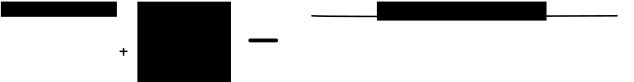
\includegraphics{Figures/pipeline.pdf}
    \caption{Overview of the pipeline of the method. The user provides as input an initial height field and sets the water level, as well as a definition of the materials properties and environmental objects properties that will be used in the iterative process. These inputs are initialized as an initial set of environmental objects and scalar fields that represents the environment values. In the iterative loop, new environmental objects are instantiated using the current state of the environment at their optimal position. The existing environmental objects in the terrain reevaluate their fitting function to grow or die and update the environment values locally. At each iteration, geological events can update the environment values, while the user can interact directly with the environmental objects. The result of the whole process is a set of environmental objects which is a sparse representation of the elements of the scene. }
    \label{fig:semantic-representation_pipeline}
\end{figure*}

The generation of the terrain is initialized using an initial height field $\height$ and a water level $\Wlevel$. The height field provides variation on the depth $\depth$, which can influence the generation process of the scene. We set $\depth = \height - \Wlevel$. \\
The list of available environmental objects $\availableObjects$, representing the different elements that can be present in the scene, are provided with their properties: type, size, generation rules, growing conditions and effects on the environment values (Section~\ref{sec:semantic-representation_environmental-objects}). \\
Finally, different materials can be defined with their properties such as diffusion speed, mass, damping factor and influence from the water currents. Materials distributions are represented as a scalar field $\material: \R^2 \to \R$ and water currents as a vector field $\Water: \R^2 \to \R^2$ that can be evaluated by the environmental objects of the scene to simulate their growth and spawn at the most probable position. The environmental properties $\environment = (\depth, \Water, \Wlevel, \material)$ is composed of depth, water currents, water level and materials distribution information at any point of the terrain (Section~\ref{sec:semantic-representation_communication}). \\
The definition of environmental objects' properties and environment properties is done with field experts, providing the pertinent parameters required to model the evolution of the terrain elements using expert knowledge (Section~\ref{sec:semantic-representation_biology}). Additional properties can easily be added to the environment properties $\environment$ in order to fit to the experts needs, such as atmospheric pressure, humidity, temperature, ... \\
The generation phase can optionally be started with an initial set of environmental objects present in the scene. 

%- Main loop \\
Once the initialization phase is done, the generation begins. The generation process is incremental and its main loop is composed of two different steps: the instantiation of new environmental objects then the update of the environment.
% - Object instantiation \\
At each iteration, new environmental objects can be created at their most fitting locations if possible. The generation rules provided in the initialization phase are used to find the optimal position from stochastic sampling (Section~\ref{sec:semantic-representation_generation-rules}). 
All environmental objects are evaluating their state analytically using the fitting function provided as input (Section~\ref{sec:semantic-representation_obj-evaluation}).
% Once the new objects are instantiated, the process can continue.
% - Environment update \\
Once the instantiation step is done, the environment's values are updated by each environmental object by deposing and absorbing some of the available materials (Section~\ref{sec:semantic-representation_materials}) while modifying the water currents (Section~\ref{sec:semantic-representation_water-currents}) around them. Finally, water currents and height field's gradient displace materials of the terrain at each iteration.
% We consider the water currents to be a steady-state flow, allowing us to remove the variation from time in the flow equations.
% The water currents are updated locally by each environmental object using an analytical form $W^*(\p) = W(\p) + \omega(\p)$.
During the generation process, the user can alter directly the distribution and shapes of the environmental objects (Section~\ref{sec:semantic-representation_manual-interaction}) and perturb the generation process by planning geological events that have impacts on the environment values (Section~\ref{sec:semantic-representation_events}).

% - Output result \\
The output of our system is a set of environmental objects disposed in the plane. We do not provide the 3D representation of the environmental objects, letting the user define the rendering method. The figures used in the paper use a mix of implicit surfaces and triangular meshes.



\subsection{Environmental objects}
\label{sec:semantic-representation_environmental-objects}

Environmental objects are rule-based objects following rules depending on their local environment for evaluation their state in their life cycle. We can see them as a life form in the way that they are created and eroded with time. During their lifetime, they influence their local environment by depositing and absorbing materials around them and influencing the water currents. The environment objects are described spatially as a single point, a parametric curve or a region.

% \subsubsection{Object's life cycle}
We consider that all environmental objects follow a life cycle of spawning, growing and dying. While many environmental objects of a terrain is not a living being, we assume that evolution of relief, for example, starts at one point in time, grow as the geological factors force it to and is eroded until a point where this environmental object can not be distinguished from the rest of the environment. 

Environmental objects are spawn stochastically in the terrain at the optimal fitting position. This position is determined from a generation rule given by the user for each of the environmental objects, which is dependant on the environment state.
Once the environmental object is present in the scene, it will continuously evaluate its fitting function to determine its state in the life cycle. If the evaluation results as less than zero, the environmental object dies and it is removed from the list of environmental objects present in the scene. While the environmental object remains, it will continue influencing its environment, by absorbing and depositing material around it and by influencing the water currents. 

\subsubsection{Generation rules}
\label{sec:semantic-representation_generation-rules}
Generation rules provides, for each environmental object, a fitting function $\fittingFuncObj$ defining the most probable location for an environmental object to spawn. Fitting functions' parameters contains, for every point $\p$, the environmental values $\environment_p$ (the amount of each material available $\material(\p)$ and the velocity and direction of the water currents $\Water(\p)$) and information about surrounding environmental objects $\objects$ (signed distance from the closest punctual environmental object or curve defining curve- and region-based environmental objects, curvature of the curve, and start and end points of the curve-based environmental objects).

% \subsubsection{Point, curve and region generation}
The seed point of a spawning environmental object is defined by a stochastic sampling of the plane. We propose different optimization means to find the optimal fitting position, depending on the environmental object shape.

The spawning position of a punctual environmental object is found at the local maxima of the fitting function from a seed point. The optimisation process simply follows the field's gradient $\nabla \fittingFuncObj$ until the local maxima is reached.

A region is defined as an isocontour of the field for which the target area $\Area$ is found. From the seed point, we follow the isolevel of the fitting function $\nabla \fittingFuncObj^\perp$ until a loop is created to define the initial condition of the shape. Using the Active Contours algorithm, we can optimize the region's energy defined as $\energy = \Einternal + \Eshape$ with  
\begin{align}
    \label{eq:internal-energy-equation}
    \Einternal = \frac{1}{2} \left( \alpha(t) \norm{\frac{d v}{d t}(t)}^2 + \beta(t) \norm{\frac{d^2 v}{d t^2}(t)}^2  \right).
\end{align}
The internal energy $\Einternal$ force the shape compact while the shape energy $\Eshape$ force the shape into a specific target. For the environmental objects generated in the following examples, we used a constraint on a target area.
\begin{align}
    \label{eq:area-target-equation}
    \Eshape = \left( \Area - \area \right)^2
\end{align}
with $a$ the current area of the shape and $\Area$ the target area, provided by the user for each shape, with some randomness.

A curve have different generation rules. It can either follow the gradient of the fitting function $\nabla \fittingFuncObj$, follow the isocontour $\nabla \fittingFuncObj^\perp$, or follow the heat points.
While the first two possibilities are trivial, the later can also be optimized using the Active Contours algorithm by optimizing the energy $\energy = \Einternal + \Eshape$ with Equation~\eqref{eq:internal-energy-equation}. We applied a length constraint on the curves : 
\begin{align*}
    \Eshape = \left( \Length - \length \right)^2
\end{align*}
with $\length$ the curve's length and $\Length$ the target length. This algorithm is sensible to the initial shape of the curve, so we start with a straight line following the isolevel at the seed point.

\subsubsection{Environment object's evaluation}
\label{sec:semantic-representation_obj-evaluation}
Environment objects are evaluated at every iteration in order to determine the current state of the life cycle of the environmental object. For punctual environmental objects, this evaluation is applied at its position $\fittingFuncObj = f(\environment_{p})$. Curve environmental objects are evaluated along the parametric curve $\curve$ such that $\fittingFuncObj = \int_{\curve} f(\environment_{\curve(t)}) \,dt$. In practice, we compute the evaluation as the average of all control points of the curve $\frac{1}{n} \sum_{i}^{n}{f(\environment_{C_i})}$.
Region environmental objects are evaluated inside their region $\domain$ as such $\fittingFuncObj = \int_{\domain} f(\environment_p) \,dp$. In practice, we compute the average of random points in the region $\frac{1}{n} \sum_{i}^{n}{f(\environment_{p_i})}$. When deformations on the environmental object's shape is applied, we apply cage deformation using Green's coordinates in order to keep consistent evaluation points during the whole life cycle of an environmental object.

% \subsubsection{Dying}
% An object spawn has a chance of disappearing if living conditions are unmet. At death, the environmental object will deposits its remains in the environment properties. \\
% We consider an object as dead when the fitting score drops to zero.
% At this point, the object is removed from the scene and materials can be deposited in the environment following the same rule as the normal step rule.

% \subsection{Communication between objects and environment}
\subsection{Environment values}
\label{sec:semantic-representation_communication}
All environmental objects of an ecosystem has an impact on all the other environmental objects, which would result in an exponentially growing computation effort as the number of environmental objects of the terrain increase. We avoid this problem by considering the environment values as a proxy to allow any environmental object to interact with any other one. Each of the environmental object have a local impact on the environment values without knowledge of neighboring environmental objects. This modification of the environment values can be due to an absorption and deposition of some material $\material$ or an influence on the water currents.


\subsubsection{Environment materials}
\label{sec:semantic-representation_materials}
The environment is composed of a scalar field for each of the possible material that can be found in the terrain. The scalar fields represents the availability of the material at any point, but not a height field. Each material is defined with a mass $\mass$, a fluid velocity factor $\velFactor$, a diffusion rate $\diffusion$ and finally a decay rate $\decay$.

Each environmental object in the terrain is a source and a sink of materials. It is the main mean of communication between environmental objects as it allows them to interact with their surrounding environment. We define the amount of deposed material with $\deposition_\material$ and $\absorption_\material$ the amount of material deposed and absorbed by the environmental object and $\growthRate(t) \in [0, 1]$ a factor related with the current state of the environmental object, which state that more material will be displaced when the environmental object is fully formed than when it was just spawn:
\begin{align*}
    \int_{0}^{t} {\growthRate(t) \left( \deposition_\material - \absorption_\material \right) \,dt}
\end{align*} 
The deposition and absorption around an environmental object is defined using the Gaussian kernel distance computation from the skeleton.

The scalar field for the material $\material$ is displaced by using a warp operator $\warp$, taking into account the water flow $\Water$ and the terrain slope $\nabla \height$. We unified the warp with $\mass$ the mass of the material and $\velFactor$ a influence factor of the fluid on the material: 
\begin{align*}
    \warp(\p, t) = \mass \nabla \height(\p, t) + \velFactor \Water(\p, t)
\end{align*}
 
% Materials are not seen as particles but more as a probabilistic distribution, so we allowed us to simplify the transport rate equations in this simpler version.
The materials are also dispersed at a diffusion rate $\diffusion$, for which we can use the advection-diffusion-reaction equation to evaluate the distribution after a time $t$
\begin{align} 
	\label{eq:material-displacement-equation}
    \frac{\partial \material}{\partial t} \warp \nabla \material = \diffusion \nabla^2 \material - \decay \material
\end{align}

We solve \eqref{eq:material-displacement-equation} numerically using Euler integration
\begin{align}
    \material(\p, t + dt) &= \material(\p, t) + dt ( \diffusion \nabla^2 \material(\p, t) - \decay \material(\p, t) \\ & - \warp(\p, t) \nabla \material(\p, t) ) \nonumber
\end{align}

The introduction of the decay rate $\decay$ in the equation allows for the reach of a steady-state, where we can consider the simulation stable. As the user updates the state of the simulation manually, we observe the reach of this steady state before continuing the iterative steps.
% Todo: explain better this steady-state phase


\subsubsection{Water currents}
\label{sec:semantic-representation_water-currents}
We define our water currents as a vector field defined as 
\begin{align*}
    \Water(\p) = \Wuser(\p) + \Wsimu(\p) + \Wobj(\p)
\end{align*}
With $\Wuser$ a user-defined vector field, $\Wsimu$ an analytical solution inspired by a wind flow simulation \cite{Paris2020}, and $\Wobj$ the water flow alteration computed from the environmental objects. 
The component $\Wsimu$ is terrain-induced. Given an input flow direction $a$, we modify the vector field by warping it with the terrain gradient smoothed at multiple scales :
\begin{align*}
    \Wsimu(\p) = \sum_{i=0}^{i=n}{c_i \warp_i \cdot v}
\end{align*}
with $v = (a (1 + k_w \depth(\p))$ and $\depth(\p)$ the depth at point $\p$ and $k_w$ a scaling factor, used to simulate the Venturi effects. $\warp_i \cdot v$ is the warping operator at scale $i$ with a coefficient $c_i$ defined as 
\begin{align*}
& \warp_i \cdot v = (1 - \alpha) v + \alpha k_i \nabla \Tilde{h_i}^{\perp}(\p) & \alpha = \norm{ \nabla \Tilde{h_i}(\p) }
\end{align*}
with $k_i$ a deviation coefficient, $\alpha$ the slope of the smoothed terrain and $\nabla \Tilde{h_i}^{\perp}(\p)$ the orthogonal vector of the smoothed terrain. As proposed by the authors, we used two scaling levels $n = 2$ with gaussian kernels of radii \si{200}{m} and \si{50}{m} with weights 0.8 and 0.2 and deviation coefficients $k_0$ and $k_1$ of 30 and 5.

$\Wobj$ is a deformation field defined as the accumulation of flow primitives \cite{Wejchert1991}. Kelvinlets are applied on each environmental objects to deflect the water flow. We use the scale and grab formulations of the regularized Kelvinlets brushes \cite{DeGoes2017}, denoted as $s_\eps(r)$ and $g_\eps(r)$ respectively to simulate obstruction and diversion, are defined as
\begin{align*}
    s_\eps(r) &= (2b - a) \left (\frac{1}{r_\eps^3} + \frac{1}{2r_\eps^5} \right)(s r) \\
    g_\eps(r) &= \left[ \frac{a - b)}{r_\eps}I + \frac{b}{r_\eps^3} r r^t + 
\frac{a \eps^2}{2 r_\eps^3} \identity \right] \force
\end{align*}
with $a = \frac{1}{4 \pi \mu}$ and $b = \frac{a}{4 (1 - \upsilon)}$ provided $\mu$ a shear modulus and $\upsilon$ a Poisson ratio provided for each Kelvinlet, $r = \p - \q$ for $\p$ the evaluation position and $\q$ the center point of the Kelvinlet, $r_\eps = \sqrt{\norm{r}^2 + \eps^2}$ the regularized distance, $\eps$ a radial scale for the deformation field, $s$ a scaling factor and $\force$ the force vector of the grab operation.
Deformations defined on curves use $\q = C(\p)$ with $C(\p)$ the closest point on the curve from the point $\p$ and $f = C'(\p)$. We can then define $u_o(\p) = s_\eps(\q - \p) + g_\eps(\p - \q)$. \\
Finally, we can retrieve the velocity field from the objects:
\begin{align*}
    \Wobj(\p) = \sum_{o \in \objects}^{}{\lambda_o u_o(\p)}
\end{align*}


\subsection{User interaction}
\label{sec:semantic-representation_interaction}
The user can guide the generation process. The use of simple shapes as environmental objects facilitate the edition of the simulation, as we can interactively add, remove or modify environmental objects, or focus the generation process in a restricted area. Interaction with the environment values is also provided as geological events, that the user can invoke during the simulation. While the direct interactions on the environmental objects are instantaneous, as a the geological events are active on a given duration.

\subsubsection{Direct interactions on the environmental objects}
\label{sec:semantic-representation_manual-interaction}
The interactive nature of our simulation enables the user to modify the state of the terrain by manipulating directly the environmental objects of the scene. We assume the modifications applied between two iterations of the simulation.

Translating an environmental object is trivial, we simply requires to evaluate the state of the environmental objects at a translated position. The deformation of environmental objects can be applied on curve and region environmental objects by updating the control points of the skeleton and recomputing the resulting implicit surfaces. The evaluation positions used for region environmental objects are displaced by applying a cage deformation of the 2D shape using the Green coordinates of points in the shape. After the alteration of the region, evaluation points should be keeping a similar distribution than before, avoiding unexpected results during the interaction.
By modifying an environmental object, the environment values may change, which can result in the destruction of the now incompatible environment objects in the scene (Figure~\ref{fig:semantic-representation_user-interaction}).

\begin{figure}
    \centering
    \includegraphics[width = 0.3 \linewidth]{Figures/Interactions/InteractionEdition1.png}
    \includegraphics[width = 0.3 \linewidth]{Figures/Interactions/InteractionEdition2.png}
    \includegraphics[width = 0.3 \linewidth]{Figures/Interactions/InteractionEdition3.png}
    \caption{Starting from a coral colony developed around a canyon (\textit{left}), the user edits the shape of the canyon, resulting in a different configuration of the scene, killing the corals that ends too deep in the water (\textit{center}) and the development and growth of new corals at the previous location of the canyon (\textit{right}). }
    \label{fig:semantic-representation_user-interaction}
\end{figure}

As long as a non-zero fitting function is defined in the terrain, new environmental objects can be forced by the user at any point of the simulation. 

% \subsubsection{Guiding the simulation}
Control over the region of the terrain that should be updated can be given by adjusting all fitting functions through a scalar field $\influence: \R^2 \to \R $ such that the fitting function $\fittingFuncObj(\p)$ of any new environmental object is evaluated as $\fittingFuncObj^*(\p) = \influence{\p} \fittingFuncObj(\p)$. This is especially useful in the planning of robotic simulations as we can first generate the overall shape of our terrain and secondly focus the generation process around the areas that may be visited by the robot, avoiding useless simulations and computer power. 
Figure~\ref{fig:semantic-representation_coral-colonization-scene} shows an example of colonization of the coral polyps that we limited manually into an annulus.
% Figure~\ref{fig:semantic-representation_focus-area-example} shows an example of colonization of the coral polyps that we limited manually.

% \begin{figure}
%     \centering
%     \includegraphics{Figures/UserControl/guidedGeneration1.png}
%     \caption{Controlling the generation area can produce a user-defined focused shape.}
%     \label{fig:semantic-representation_focus-area-example}
% \end{figure}

% - Changing the water currents \\
Our water current simulation is modeled as a simple vector field. As such, the user is able to interact with it at any moment of the simulation, allowing for the death of sensible environmental objects while it will guide the simulation into a new landscape. By modifying the water currents, the user also modifies the transport rate of materials at this position. The modification of currents is given as a stroke, a parametric curve $\curve$ for which we evaluate $\Delta \Wuser(\p)$ just as for curved environment objects (Section~\ref{sec:semantic-representation_water-currents}).

\subsubsection{Geological events}
\label{sec:semantic-representation_events}
A configuration file can define in advance the different events that should be triggered during the simulation. This can be useful to generate landscapes that are close to some existing locations. 
Multiple geological events can be triggered either as sudden or continuous environmental changes. These changes play a huge role in the morphology of landscapes.
We define events with a starting point and an ending point, such that at any time of the simulation we can compute the progress of the event as $\tEvent \in [0, 1]$.

Water level changes are important events that shape the underwater landscapes. As previously submerged environmental objects get elevated above water level, flora and fauna terrain elements dry and die. Deprived from the living part of the elements, everything is more affected by terrestrial erosion. By updating the value of the depth $\depth$ evaluated in the fitting functions, any environmental object that is sensible to the depth will be impacted automatically, that may be causing death (Figure~\ref{fig:semantic-representation_water-event}). The modification of the water level is defined as 
\begin{align*}
    \depth(\p) = \depth_0(\p) + \sum_{e \in \events} \Delta \depth_e \tEvent
\end{align*}
with $\Delta \depth_e$ the amount of water rising or lowering during an event. We assumed a linear evolution of the water level during an event. This allows to evaluate the depth at any point in space and in time.

\begin{figure}
    \centering
    \includegraphics[width = 0.45 \linewidth]{Figures/Interactions/InteractionWater1.png}
    \includegraphics[width = 0.45 \linewidth]{Figures/Interactions/InteractionWater3.png}
    \caption{Lowering the water level by a few meters caused most of the coral objects to satisfy $\fittingFuncObj \leq 0$, causing their death. Since the water level (blue) decrease slowly, new coral objects spawn progressively at a lower altitude.}
    \label{fig:semantic-representation_water-event}
\end{figure}

Subsidence and uplift are the main geological events that create or destroy islands in the long term. These events are simulated as a simple factor on the height field of the generated terrain (Figure~\ref{fig:semantic-representation_subsidence-event}). Subsidence is not always uniform in the terrain. As such, the user can provide a position $\q$ at which the subsidence is the strongest, the amount of subsidence applied $\Delta \height_e$ and a standard deviation $\std$ for which we can then compute at any point in space and time of the simulation the height of the terrain
\begin{align*}
    \height(\p) = \height_0(\p) \cdot \sum_{e \in \events}{\frac{G(\norm{\p - \q})}{G(0)}} \Delta \height_e \tEvent 
\end{align*}
with $G(x)$ the Gaussian function
\begin{align*}
    G(x) = {\frac {1}{\std {\sqrt {2\pi }}}} \exp \left(-\frac {x^{2}}{2 \std ^{2}}\right)
\end{align*}

\begin{figure}
    \centering
    \includegraphics[width = 0.45 \linewidth]{Figures/Interactions/InteractionSubsidence1.png}
    \includegraphics[width = 0.45 \linewidth]{Figures/Interactions/InteractionSubsidence2.png}
    \caption{Simulating subsidence on a part of the terrain (brown area) cause the depth value to change locally, resulting in the death of coral objects that find themselves too deep to survive. Here two subsidence events are triggered in parallel. }
    \label{fig:semantic-representation_subsidence-event}
\end{figure}

Storms are factors of the geomorphology of coral reefs \cite{VilaConcejo2016, Oron2023} and coasts \cite{Dominguez2005, Cowart2010}. Due to the extreme wind and wave velocities coasts are highly eroded in a short time period and the more fragile corals near the water surface are broken, possibly causing breaches in the reefs and spreading polyps in the currents direction. While there are many factors at play to understand the apparition of storms and the hydrodynamics affecting it, we simplified the model of storms to the user as a single epicenter $\q$ with a wind velocity $\windVelocity$ and a standard deviation $\std$ representing the spread around the epicenter (Figure~\ref{fig:semantic-representation_storm-event}). The computation of water currents are then computed as 
\begin{align*}
    \Wuser(\p) = \Wuser^*(\p) + \sum_{e \in \events | \tEvent \in [0, 1]} {\windVelocity \frac{G(\norm{\p - \q}}{G(0)}}
\end{align*}
In this case, we did not include the linear factor $\tEvent$ as storms are usually conserving a constant force for the time of the few weeks or months of their occurrence. 

\begin{figure}
    \centering
    \includegraphics[width = 0.45 \linewidth]{Figures/Interactions/interactionStorm1.png}
    \includegraphics[width = 0.45 \linewidth]{Figures/Interactions/interactionStorm2.png}
    \caption{The result of a storm localized on one side of the island (red area) modifies the result of the evaluation of environmental objects around its epicenter for a short period of time. Most of the coral objects died from the event, except few environmental objects less sensible to water currents strength. }
    \label{fig:semantic-representation_storm-event}
\end{figure}

% Just as for the rise and lowering of water level, the heat is modeled as a simple value of the environment. For shallow areas (<100m) we assume a linear relation between depth and temperature, and a constant value for the terrestrial environment. As such, we can model a heat wave by a change of the environment values. Environmental objects who are sensible to temperature may die instantly. The modification of the temperature is defined as 
% \begin{align*}
%     \temperature(\p) = T_0(\p) + \sum_{e \in events} \Delta \temperature_e \tEvent + c \depth(\p)
% \end{align*}
with $\Delta \temperature_e$ the change of heat during an event, $\temperature_0$ the temperature at the water surface, and $c$ a very small factor.

The framework can easily be extended as the geological event system stays similar for all events. Including higher level simulations in the event system can be added, such as the simulation of tectonic activity, the use of fluid dynamics for tsunami events, the integration of human activity, ...

\section{Expert knowledge integration}
\label{sec:semantic-representation_biology}
  The definition of the fitting functions of the environmental objects are inspired by the biological and geological factors that rule the evolution of underwater landscapes. The main factors are depth, light, water currents and biodiversity. External events have direct and indirect repercussions on the biodiversity of underwater environments. Coral islands are complex bio systems in which fauna, flora and geology are mixed together. 

\subsection{Environmental objects description}
\label{sec:semantic-representation_represented-objects}
We have represented with environmental objects some geologic elements, animal elements and flora elements. The low island is most often raised in a circular shape as the process mainly appear around a hot spot under the ground. The evolution of an island into a coral island requires that the environmental conditions are sufficient for coral development: corals will grow slightly below the water surface as waves will break its growth and at a shallow depth (around 3m to 30m deep) in order for light to reach it. As coral grow and die, the skeleton is transformed into porous limestone, providing shelter to surrounding animals and reducing the impact of water erosion on the island. Corals drop polyps that are transported by the water flow and when they stick to a hard surface, as a rock or the reef itself, the coral may grow and colonize the area. As subsidence cause the island to lower, the living part of the coral reef keep growing toward light, which lead to a reef that is constantly close to the water level without reaching it due to wave erosion. The survival of reefs depends on the equilibrium between coral growth and and erosion. Eroded parts of the reef falling in the sheltered part of the reef accumulates, ending up by forming a lagoon. An island formed by a hot spot will inevitably subside in time, until it is completely flatten. As the coral reefs keep growing, only the lagoon remain, resulting in an atoll. \\
In this work we we integrate the biological and geological knowledge in the fitting functions of the environmental objects we want to generate. We represent the islands as regions that can be appearing with a uniform distribution. From the formulation of the region description \eqref{eq:internal-energy-equation}, we mostly create circular islands. The coral elements, environmental objects described as a single point, have a fitting function that take into account the depth of the ground, the amount of sand, fresh water and polyps in their environment, as well as the strength of water currents. Each coral species have different living conditions, but we reduced our work to soft coral which are sensible to water strength and stony corals that are more resistant to erosion. Reefs are formed as coral's skeleton are transformed into calcareous stone, describing then as an environmental object representing multiple others. 

\subsection{Simplifications}
\label{sec:semantic-representation_simplifications}
The environmental factors simulated are greatly simplified as the real processes are in a very small time scale, that computer simulation are not able to simulate in interactive time. The use of environmental objects aim to represent a plausible results, while avoiding modeling the smaller scale events. Examples of simplifications are the geometry and material of each environmental object, which have an influence on the water currents through friction, the water currents represented as stationary flows, while the water flow dynamics are a complex system that may change completely at two different times of the day, the animal influence on the reefs that they transform by the ingestion and deposition of sediments, ...


\section{Results}
\label{sec:semantic-representation_results}
Our method provides a way to generate scenes at different scales. We demonstrate this capacity with the generation of a large scene of an island (Figure~\ref{fig:semantic-representation_teaser}) after what we focused the generation process in a canyon (Figure~\ref{fig:semantic-representation_canyon-scene}), then a small-scale visualization of coral colonies (Figure~\ref{fig:semantic-representation_coral-colonization-scene}).
In the examples, we rendered the environmental objects as a implicit tree or as individual meshes. The island, lagoons, reefs, canyons and sand ripples as implicit surfaces

% \subsection{Mid-scale}
% \label{sec:semantic-representation_mid-scale}
A canyon scene can be generated using our method. The water flow is affected by the curve of the canyon such that the currents are oriented in the direction of the curve's tangent.In this example, we force the position of arches to be inside the canyon. The arches deposits a material "rock deposit", which is the main element of the fitting function of the Rock object. The "rock deposit" is slightly affected by water currents, but its mass make it highly affected by gravity. As such, rocks will spawn underneath arches. In reality, an arch is often created as part of a large coral boulder that sees the calcareous bottom part detached by the water currents, often resulting in an arch surrounded by big rocks and smaller rocks from the erosion of the first rocks.
As such, we define an environmental object "Arch" with a fitting function $\fittingFunc_{arch}(\p) = 5 - d(canyon - \p) * \norm{\Water(\p)}$, an environmental object "Rock" using $\fittingFunc_{rock}(\p) = \material_{rock\_deposit}(\p)$ and Pebble using $\fittingFunc_{pebble}(\p) = \material_{smaller\_rock\_deposit}(\p)$. Finally, sand ripples are simply described as curves appearing where there is a lot of sand available: $\fittingFunc_{ripple}(\p) = \material_{sand}(\p)$.
Following these simple rules, Figure~\ref{fig:semantic-representation_canyon-scene} shows the emergence of details in the scene. 

% \subsection{Small-scale}
% \label{sec:semantic-representation_small-scale}
In this example we defined three different types of corals, coralA, coralB and coralC, to illustrate the possibility to model behaviours from the choice of fitting functions. Each of the coral types deposits a material "coral polyp" and "coral polyp A" ("coral polyp B" and "coral polyp C" respectively). By considering a fitting function that minimize the ratio $\frac{\text{coral polyp}}{\text{coral polyp A}}$, we can see an emergent behavior of the three types of coral fighting for the space colonization.
Figure~\ref{fig:semantic-representation_coral-colonization-scene} shows the result of this simulation at three different interations. At the border between two colonies, none of the colonies make progression due to the amount of coral polyp specific from the other colony.

\begin{figure*}
    \centering
    \includegraphics[width=0.245 \linewidth]{Figures/Colonization/col0.png}
    \includegraphics[width=0.245 \linewidth]{Figures/Colonization/col1.png}
    \includegraphics[width=0.245 \linewidth]{Figures/Colonization/col2.png}
    \includegraphics[width=0.245 \linewidth]{Figures/Colonization/col3.png}
    \caption{Three colonies of coral (red, blue, green) restricted to an annulus the middle section of the terrain fighting for the space.}
    \label{fig:semantic-representation_coral-colonization-scene}
\end{figure*}

\begin{figure*}
    \centering
    \includegraphics[width = 0.24 \linewidth]{Figures/Canyon/Canyon2.png}
    \includegraphics[width = 0.24 \linewidth]{Figures/Canyon/Canyon3.png}
    \includegraphics[width = 0.24 \linewidth]{Figures/Canyon/Canyon4.png}
    \includegraphics[width = 0.24 \linewidth]{Figures/Canyon/Canyon5.png}
    \caption{Evolution of a canyon scene at different iterations of the simulation. The apparition of an arch causes the spawning of rocks, pebbles, and finally some deposition of sand at the bottom of the canyon, spawning ripples. }
    \label{fig:semantic-representation_canyon-scene}
\end{figure*}



\section{Discussion}
\label{sec:semantic-representation_discussion}
The proposed method aims to generate plausible landscapes using simplified versions of the evolution of an ecosystem and of the 3D representation. The biological realism of the result is highly correlated to the amount of simplification and assumptions, while the visual realism is completely dependent to the geometric functions used for the 3D modeling of the environmental objects. While proposing a flexible method that propose a generic approach for terrain generation, a close collaboration with fields experts and with graphists is needed to achieve optimal results.

Most simulation algorithm's quality depends on the size of the time step used, but with the introduction of a decay rate in the materials properties, we limit the influence of time steps by considering that steady-state are reachable. The material deposition and absorption on punctual environmental objects can be seen as a Dirac function $\dirac$ centered at their position resulting in the advantage that material displacement function can use the definition of the diffusion equation instead of the advection-diffusion-reaction equation. This equation allowing us to evaluate the state of the material $\material$ without intermediate steps, but this is not applicable with curve- and region-based environmental objects. 

\section{Conclusion}
\label{sec:semantic-representation_conclusion}
We have proposed a method to generate terrains procedurally using sparse representations. This representation, the environmental objects, enables to introduce expert knowledge by the mean of the fitting functions that rule the environmental objects life cycle, but also to integrate the user in the loop during the generation process. We reduced the terrain resolution limitations by defining the environment objects as parametric elements. Thanks to the sparse representation based on single points, curves and regions, we allow for direct manipulation of the environmental objects of the scene by the user which, thanks to the environment steady state consideration, also enables to include these interactions in the automatic simulation process. \\
Integrating environmental properties in the fitting function of environmental objects allows the user to guide the generation through geological events. Our method enables each environmental object of the scene to influence the environment locally, reducing the need of computations while also retrieving environment values locally, which result in a parallelizable life-like simulation process. The genericity of the environment properties definitions should be sufficient for plausible generation of other landscape types as long as expert knowledge can be translated to environmental object's formalism.


We limited our work to the use of 2D scalar fields as they are more easily differentiable, interpretable and lighter than volumetric representations. However, future works include using 3D representations of the terrain and the environment to generate 3D terrains, including cavities, sub-terrestrial areas and the interior of coral structures. 
% The different possibilities to explore for this would be: the use of 3D particles to represent the state of the materials in the environment, or voxel grids or flatten representation of the terrain's surface (but would not allow a different morphological shape than the height field...).

\def\url#1{} % This line actually remove the "URL" link from the references


\begin{figure*}
    \centering
    \includegraphics{Figures/CoralIsland/multiScene1 v2 final 1.png}
    \caption{A simple coral island is generated using an island, a lagoon, reefs coral polyps, beaches, trees and algae environmental objects. Trees appear on beaches and algae grow in the lagoon's sand. }
    \label{fig:semantic-representation_coral-island-scene}
\end{figure*}

% bibtex
%\bibliographystyle{eg-alpha-doi}
%\bibliography{references_terrain}

% biblatex with biber
% \printbibliography

%\end{document}
%
%- Qu'est-ce qu'une representation sémantique ? \\
%** Définition linguistique + Définition image + notre définition \\
%- Pourquoi une representation semantique? \\
%** Partage de connaissances avec biologistes, geologues, etc... \\
%** Données de carnets de voyages, cartes labellisées, ... \\
%- Avantages et inconvéniants de la representation sémantique \\
%** Avantages: \\
%*** Interpretation \\
%*** Control utilisateur \\
%*** Abstraction representation 3D \\
%** Inconvéniants: \\
%*** Besoin de connaissances experts (+ problèmes communication interdisciplinaire) \\
%*** Simplifications nécessaires sur la physique / phénomènes naturels \\
%- Representation 3D des terrains semantiques \\
%** Mélanges de méthodes possibles (fonctions implicites + maillages)
%
%\section{Representation de terrain parsemée}
%- Paysage contient des structures de tailles très variables :\\
%** Montagnes sur plusieurs km² mais rivières larges de quelques mètres, par exemple \\
%- Proposition de representation du terrain de manière parsemée \\
%** Definition des éléments du terrain par un objet simple : objets environementaux \\
%** Géométrie implicite, proposant un affichage 2D ou 3D \\
%** Possibilité "facile" de LOD \\
%- Méthode de génération itérative de terrain parsemé \\
%** Reduire temps de calcul $O(n^2)$ à $O(n)$ par l'utilisation de l'environnement comme proxy\\
%** Méthode basée sur la déposition de matériaux \\
%** Processus stochastique itératif
%
%\section{Objets environnementaux}
%- Symbolique de l'objet environnemental \\
%- Reference "Environmental Objects" \\
%- Comparaison aux biotopes
%
%\subsubsection{Definition}
%- Squelette \\
%- Forme paramétrique \\
%- Conditions de vie
%
%\subsubsection{Implémentation}
%- Instantiation des objets \\
%** Definition du squelette \\
%*** Points, courbes, régions \\
%*** Utilisation Snake
%** Definition geométrie \\
%- Modifications sur environnement \\
%- ...
%
%% \newcommand{\Esnake}{E_{\text{snake}}}
\newcommand{\Eintern}{E_{\text{internal}}}
\newcommand{\Eextern}{E_{\text{external}}}
\newcommand{\Econt}{E_{\text{cont}}}
\newcommand{\Eimage}{E_{\text{image}}}
\newcommand{\Ecurv}{E_{\text{curv}}}

\subsection{Snake - Modèle de contour actif}

Nous souhaitons symboliser une zone de corail mort comme étant un objet environemental "récif".Pour cela, les objets corail déposent continuellement une quantité de materiau "corail mort". Ce materiau, stocké dans un champ scalaire discret, contient alors de fortes intensités là où un récif devrait, semblerait-il, exister.
Il faut alors tracer une courbe pour représenter ce nouvel objet. Les contraintes de cette courbe est qu'elle doit traverser les points de plus haute intensité, tout en conservant une longueur donnée.
L'algorithme de Snake, ou Active Contour Model (Modèle de Contour Actif en français) s'approche de cette application. L'algorithme propose de donner une énergie à la courbe, qui essaie alors de la minimiser par descente de gradients.
L'énergie, dans le papier initial est défini  par 
$$
\Esnake^{*} = \int \limits _{0}^{1} \Esnake(\mathbf {v} (s))\,ds = \int \limits _{0}^{1} \left( \alpha + \beta \right) \Eintern (\mathbf {v} (s)) + \gamma \Eimage (\mathbf {v} (s)) + \Econt (\mathbf {v} (s)))\,ds
$$
L'énergie interne représente les propriétés de la courbe : 
$$
\Eintern = \alpha \Econt + \beta \Ecurv
$$
Le coût de continuité $\Econt$, originellement definit comme la minimisation de l'espacement entre les points $\left\|{\frac {d{\bar {v}}}{ds}}(s)\right\| ^{2}$, n'a pas beaucoup de sens dans la forme discrète de l'algorithme. Dans sa forme discrète on cherche à conserver un interval régulier entre les points en appliquant $\Econt = \left(\tilde{d} - \left\|p_i - p_{i-1} \right\| \right)^2$ avec $\tilde{d}$ la distance moyenne entre chaque point.

Le coût de courbure $\Ecurv$ cherche à minimiser les oscillations de la courbe et peut alors se définir comme la derivée seconde au carré $\left\|{\frac {d^{2}{\bar {v}}}{ds^{2}}}(s)\right\| ^{2}$.
La forme discrète $\Ecurv^{*} = \left\| p_{i-1} - 2 p_i + p_{i+1} \right\| ^2$ n'est pas nécessaire avec des splines, dû à leur forme close.

Le coût d'image $\Eimage$ essaie d'attirer les points de la courbe vers un maximum local du gradient de l'image. On le définit par $\Eimage = - \left\| \nabla I \right\| $

Nous souhaitons voir notre courbe garder une longueur donnée $L$. On modifie alors la formulation du cout de continuité pour devenir $\Econt = \left(\tilde{l} - \left\|p_i - p_{p-1} \right\| \right)^2$ avec $l = \frac{L}{n - 1}$ sachant $n$ le nombre de sommets de la courbe. De plus, on souhaite une courbe qui suit les points de haute intensité plutôt que le gradient, ce qui revient à modifier le coût d'image $\Eimage = -I$.

Le calcul du gradient $\nabla \Esnake$ reste trivial par parties :
\begin{align*}
	\frac{\partial \Eimage}{\partial p_i} &= - \nabla I(p_i) \\
	\frac{\partial \Ecurv^{*}}{\partial p_i} &= -\frac{2 \left( p_{i-1} - 2 p_i + p_{i+1} \right) }{ \left\| p_{i-1} - 2 p_i + p_{i+1} \right\| } \\
	\frac{\partial \Econt^{*}}{\partial p_i} &= 2 \left(l - \left\|p_i - p_{i-1} \right\| \right) \cdot \frac{p_i - p_{i-1}}{ \left\| p_i - p_{i-1} \right\| }
\end{align*}

Nous avons alors
\begin{align}
	\Esnake &= \alpha \left(l - \left\|p_i - p_{i-1} \right\| \right)^2 + \beta \left\| p_{i-1} - 2 p_i + p_{i+1} \right\| ^2 - \gamma I \\
	\nabla \Esnake &= 2 \alpha \left(l - \left\|p_i - p_{i-1} \right\| \right) \cdot \frac{p_i - p_{i-1}}{ \left\| p_i - p_{i-1} \right\| } - \beta \frac{2 \left( p_{i-1} - 2 p_i + p_{i+1} \right) }{ \left\| p_{i-1} - 2 p_i + p_{i+1} \right\| } - \gamma \nabla I(p_i)
\end{align}

Il est à noter que le calcul de $\Econt^{*}$ utilise la distance $\left\|p_i - p_{i - 1} \right\|$. Pour $i = 0$, on utilise la distance $\left\| p_i - p_{i + 1} \right\|$.
Si tous les points de la courbe sont à une distance supérieure à $l$, l'optimisation poussera chacun de ces points à se rapprocher son point prédécesseur. Le point $p_0$, lui, ne se déplacera très peu, donc l'ensemble de la courbe se cale vers le point $p_0$. En utilisant la distance vers le successeur $\left\| p_i - p_{i+1} \right\|$, la courbe se déplace en direction du point $p_N$.
Il est alors possible de converger vers le point médian en alternant l'utilisation de distance avec le prédécesseur et avec le successeur, au coût d'une convergence plus lente.

L'algorithme de modèle de contour actif est fortement sensible à l'emplacement de la courbe de départ. Dans le cas où une portion de la courbe se situe dans un endroit à très faible gradient sur $\Eimage$, les sommets de la courbe vont simplement optimiser $\Eintern$, résultant en un segment droit, dans une zone à faible intensité, tandis que le reste de la courbe s'optimise correctement.
Afin de limiter ce problème, on propose d'adapter l'algorithme Snake en Catapillar: tout au long de la descente de gradient, on réduit puis agrandit artificiellement la longueur cible $L$. De cette manière, une portion de courbe bloqué dans une région sans optimisation possible sur l'energie externe sera attirée par la courbe optimisée jusqu'à retomber sur un gradient fort. La portion morte peut prendre la place des sommets optimisés. En ramenant la longueur cible $L$ à la valeur initiale, l'optimisation est continuée avec des sommets en moins dans la zone morte. La répétition de ce procédé permet de ramener, petit à petit, tous les points en zone optimisable. Néanmoins, un changement trop rapide de la longueur cible peut empêcher les sommets d'optimiser $\Eextern$ en amplifiant trop $\Eintern$. De plus, cet algorithme peut amener à des erreur numeriques et une convergence ralentie.


%
%
%\subsection{Communication entre objets}
%- Comparaisons avec réalité \\
%** Pas de communication directs entre les éléments \\
%- ...
%
%\subsubsection{Échanges par l'environnement}
%- Modifications de l'environnement \\
%** Absorption \\
%** Deposition \\
%** Modification des courants \\
%- Impact de l'environnement sur les objets \\
%- ...
%
%\subsubsection{Cycle de vie des objets environnementaux}
%- ...
%
%\section{Résulats}
%- ...


%\subsection{Outils implémentés}
%- Parseur de fonctions de coût \\
%- ...

%\section{Autre tentative}
%\subsection{Échanges directs}
%\subsubsection{Génération de graphe}
%\subsubsection{Triangulation de Delaunay}


%
%\section{Érosion continue}
%[POSSIBLEMENT À DEPLACER DANS EROSION] \\
%- ...
%
%\subsection{Description du problème}
%- Processus d'érosion est un système dynamique \\
%- Nombre de variables très important \\
%- Impossible de simuler à des pas de temps différents et/ou à différentes échelles/résolutions
%
%\subsection{Solutions proposées}
%- ...
%
%\subsubsection{Cycle de vie des objets environnementaux}
%- ...
%
%\subsubsection{Utilisation d'apprentissage profond}
%- ...




%\chapter{Génération de biotopes}
\minitoc

- ...

\section{Définition}
- ...

\subsection{Récursivité}
- ...

\subsection{Diagramme de Voronoï}
- ...

\subsection{Communication entre biotopes}
- ...


%- ...
%
%\section{Génération de biotopes}
%- ...
%
%\subsection{Définition}
%- ...
%
%\subsubsection{Récursivité}
%- ...
%
%\subsubsection{Diagramme de Voronoï}
%- ...
%
%\subsubsection{Communication entre biotopes}
%- ...
%


\part{Modelisation}

\chapter{Modélisation de terrains volumiques [PEUT ETRE A DEPLACER DANS INTO]}
\minitoc

- Volumique est important pour représenter les structures en 3D \\
- Permet de representer des cavités, des arches, des superpositions, ... \\
- Notion de matériaux permet d'inclure beaucoup plus d'informations pour les parties suivantes : amplification et rendu \\
** Amplification (eg. érosion) doit connaitre le type de sol à la surface et sous-terrain pour être réaliste \\
** Rendu doit connaitre le matériau à la surface pour afficher correctement des textures \\
- ...


\section{Terrains implicites avec matériaux}
- ...

\subsection{Densité de matière}
- ...

\subsubsection{Granularité de matériaux}
- ...

\subsubsection{Soil triangle}
- ...

\subsection{Fonctions scalaires}
- ...

\subsection{Fonctions de mélange}
- ...

\subsection{Fonctions de placement}
- ...

\subsection{Utilisation de matériaux}
- ...

\subsubsection{Définition du matériau final}
- ...

\subsubsection{Post-processing : transformation de matériaux}
- ...



\section{Représentation graphique des objets environnementaux}
- Surfaces implicites \\
- Maillages \\
- ...


\chapter{Génération automatique d'îles coralliennes}
\minitoc

- Definition ile corallienne \\
- Presentation coraux \\
- Difference paysages normaux \\
** Notion de coraux \\
*** Evolution longue (ile) et courte (coraux) \\
**** Processus geologique affaissement de l'ile \\
- ...

\section{Théorie darwinienne}
- Plusieurs théories \\
- Impossibilité d'étudier aisément les environnements \\
** Utilisation d'observations \\
- Théorie réfutée par \cite{Droxler2021} \\
** Mais trop tôt pour juger \\
** Pratique dans notre cas. \\
- ...

\subsection{Multiples théories}
- 

\subsection{Voyage de Darwin}
- ...
\section{Génération d'exemples}
- ...
\subsubsection{Pipeline}
- ...
\subsubsection{Entrée}
- ...
\subsubsection{"Simulation"}
- ...
\subsubsection{Sortie}
- ...
\section{cGAN}
- ...
\subsection{Définition cGAN}
- ...
\subsection{Pourquoi un cGAN?}
- ...
\subsection{Entraînement}
- ...
\subsubsection{Utilisation de données synthétiques}
+ Problème des données synthétiques \\
- ...
\subsubsection{Augmentation de données}
- ...
\subsection{Utilisation du modèle}
- ...
\subsubsection{Génération par sketch}
- ...
\subsubsection{Temps interactifs}
- ...
\subsubsection{Réalisme}
- ...



\chapter{Génération de réseaux karstiques}
- ...

\section{Géologie}
- ...

\subsection{Formation}
- ...

\subsection{Intérêts}
- ...

\subsection{Place des karsts dans le projet}
- ...

\section{Contrôle utilisateur}
- ...

\subsection{Méthode existante}
- ...

\section{Ma méthode}
- ...

\subsection{Karst en tant qu'arbre?}
- ...

\subsection{Génération de végétation -> Space colonization}
- ...




\part{Simulation d'érosion}

\chapter*{Abstract}
- Travail réalisé en début de thèse \\
- Choix de représentation encore incertain \\
- Recherche d'abstraction de la représentation \\
** Pousse à la généralisation du système d'érosion


\graphicspath{ {./Chapter 3/figures/erosion/}{./Chapter 3/figures/terrain_representations/}{./Chapter 3/results/}{./Chapter 3/otherPapersRepro/} {./Chapter 3/images/erosion_processes/}}

\newcommand{\referenceExemple}[1] {\textit{\cref{tab:erosion-result_figures}: #1}}
\newcommand{\addingFiguresToCell}[4]{%
        \autofitgraphics[width=0.2\textwidth]{#1}
        \autofitgraphics[width=0.2\textwidth]{#2}
        \ifx\relax#3\relax
        \else
            \autofitgraphics[width=0.2\textwidth]{#3}
        \fi
        \ifx\relax#4\relax
        \else
            \autofitgraphics[width=0.2\textwidth]{#4}
        \fi
}

% The columns :
% Name & Results & Terrain representation & Dimensions & particles / iteration & iterations & particle radius & coefficient of restitution & particle density & capacity factor & erosion factor & deposition factor & Velocity field & computation time
\newcommand{\exampleCoastal}{
Coastal & \addingFiguresToCell{Coastal_1.png}{Coastal_2.png}{Coastal_3.png}{} & \densityVox & 100x100x30 & 10 & 80 & 3 & 5 & 0.1 & 500 & 10.0 & 5.0 & 0.5 & Uniform & 0.5
}
\newcommand{\exampleGlacier}{
Glacier & \addingFiguresToCell{Glacier1.png}{Glacier2.png}{Glacier3.png}{Glacier4.png} & \heightmap & 100x100 & 20 & 80 & 3 & 10 & 0.1 & 500 & 1.0 & 1.0 & 1.0 & None & 0.8
}
\newcommand{\exampleLandslide}{
Landslide & \addingFiguresToCell{Glacier_2_1.png}{Glacier_2_2.png}{Glacier_2_3.png}{Glacier_2_4.png} & \heightmap & 100x100 & 20 & 200 & 10 & 2.5 & 0.2 & 500 & 0.1 & 1.0 & 1.0 & None & 4
}
\newcommand{\exampleHydraulic}{
Rain & \addingFiguresToCell{Hydraulic1.png}{Hydraulic3.png}{Hydraulic5.png}{Hydraulic7.png} & \heightmap & 100x100 & 20 & 100 & 10 & 1.0 & 1.0 & 1000 & 10.0 & 2.5 & 0.3 & None & 4.0
}
\newcommand{\exampleKarstBinary}{
Karst & \addingFiguresToCell{KarstBinaryWithMarchingCubes1.png}{KarstBinaryWithMarchingCubes2.png}{KarstBinaryWithMarchingCubes3.png}{KarstBinaryWithMarchingCubes5.png} & \binaryVox & 100x100x50 & 2 & 1000 & 40 & 5 & 0.5 & 500 & 10.0 & 5.0 & 0.5 & Uniform & 20
}
\newcommand{\exampleKarstBinaryStrata}{
Karst & \addingFiguresToCell{KarstWithStrataNoise1.png}{KarstWithStrataNoise2.png}{KarstWithStrataNoise3.png}{KarstWithStrataNoise4.png} & \binaryVox & 100x100x50 & 2 & 80 & 3 & 10 & 0.1 & 500 & 10.0 & 5.0 & 1.0 & Uniform & 0.8
}
\newcommand{\exampleLabyrinthOF}{
Glacier & \addingFiguresToCell{LabyrinthOpenFOAM1.png}{LabyrinthOpenFOAM2.png}{LabyrinthOpenFOAM3.png}{LabyrinthOpenFOAM4.png} & \densityVox & 100x100x40 & 2 & 80 & 3 & 10 & 0.1 & 500 & 1.0 & 1.0 & 1.0 & SIMPLE\cite{Caretto1973} & 0.8
}
\newcommand{\examplePipes}{
Tunnel & \addingFiguresToCell{Pipes01.png}{Pipes05.png}{Pipes09.png}{Pipes11.png} & \densityVox & 100x100x50 & 1 & 100 & 100 & 2.5 & 0.1 & 500 & 1.0 & 1.0 & 1.0 & None & 0.8
}
\newcommand{\exampleRiver}{
River & \addingFiguresToCell{River1.png}{River2.png}{River3.png}{River4.png} & \heightmap & 100x100 & 5 & 100 & 50 & 1.5-5 & 0.5 & 900 & 0.1 & 1.0 & 1.0 & None & 2.5
}
\newcommand{\exampleRiverTwo}{
River & \addingFiguresToCell{River_2_1.png}{River_2_2.png}{River_2_3.png}{River_2_4.png} & \heightmap & 100x100 & 5 & 100 & 50 & 1.5-5 & 0.5 & 900 & 0.1 & 1.0 & 1.0 & None & 2.5
}
\newcommand{\exampleRiverWater}{
\makecell{River
(with water
level)} & \addingFiguresToCell{RiverWater1.png}{RiverWater2.png}{RiverWater3.png}{RiverWater4.png} & \heightmap & 100x100 & 5 & 100 & 50 & 1.5-5 & 0.5 & 900 & 0.1 & 1.0 & 1.0 & None & 2.5
}
\newcommand{\exampleRiverObstacle}{
\makecell{River 
with obstacle} & \addingFiguresToCell{RiverWithObstacle1.png}{RiverWithObstacle2.png}{RiverWithObstacle4.png}{RiverWithObstacle6.png} & \heightmap & 100x100 & 5 & 100 & 50 & 1.5-5 & 0.5 & 900 & 0.1 & 1.0 & 1.0 & None & 2.5
}
% \newcommand{\exampleWaterCurrents}{
% Underwater & \addingFiguresToCell{WaterCurrent1.png}{WaterCurrent2.png}{WaterCurrent4.png}{WaterCurrent6.png} & \heightmap & 100x100 & 10 & 100 & 50 & 2.5 & 0.9 & 1000 & 1.0 & 1.0 & 1.0 & \cite{Stam2003} & 4
% }
\newcommand{\exampleWaterCurrents}{
Underwater & \addingFiguresToCell{WaterCurrent1.png}{WaterCurrent2.png}{WaterCurrent4.png}{WaterCurrent6.png} & \heightmap & 100x100 & 10 & 100 & 50 & 2.5 & 0.9 & 1000 & 1.0 & 1.0 & 1.0 & [Stam2003] & 4
}
% \newcommand{\exampleWindErosion}{
% Wind & \addingFiguresToCell{WindErosion1.png}{WindErosion2.png}{WindErosion4.png}{WindErosion5.png} & \densityVox & 100x100x50 & 0.2 & 100 & 10 & 1.5 & 0.9 & 1.5 & 1.0 & 1.0 & 1.0 & \cite{Paris2019b} & 0.5
% }
\newcommand{\exampleWindErosion}{
Wind & \addingFiguresToCell{WindErosion1.png}{WindErosion2.png}{WindErosion4.png}{WindErosion5.png} & \densityVox & 100x100x50 & 0.2 & 100 & 10 & 1.5 & 0.9 & 1.5 & 1.0 & 1.0 & 1.0 & [Paris2019] & 0.5
}
\newcommand{\exampleVolcano}{
Volcano & \addingFiguresToCell{Volcano_2_1.png}{Volcano_2_2.png}{Volcano_2_3.png}{Volcano_2_4.png} & \densityVox & 100x100x40 & 50 & 150 & 30 & 1.0 & 5.0 & 2000 & 1.0 & 1.0 & 5.0 & None & 0.8
}
\newcommand{\exampleMeanders}{
Meanders & \addingFiguresToCell{meanders_base.png}{meanders_fin.png}{}{} & \implicit & N/A & N/A & 10 & 20 & 5.0 & 1.0 & 1000 & 1.0 & 1.0 & 1.0 & $^{(1)}$ & 1
}


\chapter{Erosion simulation}
\label{chap:erosion}

\teaser {
	\autofitgraphics{teaser.pdf}
	\caption{Applying shading and textures on the generated geometry can produce a plausible aspect of a coast eroded by waves on a long timespan, or a desertic landscape eroded by wind, or a mountainous area flatten by thermal erosion.}
	\label{fig:erosion-closerImage}
}

\abstract
% - Work carried out at the beginning of the thesis 

% - Representation choice still uncertain 

% - Search for abstraction of the representation 

% ** Drives the generalization of the erosion system

In this chapter, we present a novel particle-based method for simulating erosion on various terrain representations, including height fields, voxel grids, material layers, and implicit terrains. Our approach breaks down erosion into two key processes (terrain alteration and material transport) allowing for flexibility in simulation. We utilise independent particles governed by basic particle physics principles, enabling efficient parallel computation. For increased precision, a vector field can adjust particle speed, adaptable for realistic fluid simulations or user-defined control. We address material alteration in 3D terrains with a set of equations applicable across diverse models, requiring only per-particle specifications for size, density, coefficient of restitution, and sediment capacity. Our modular algorithm is versatile for real-time and offline use, suitable for both 2.5D and 3D terrains.
\pagebreak

\minitoc

\section{Introduction}
Automated terrain generation is a key component of natural scene digital modelling for animated movies and video games. A standard approach is to first generate a base terrain geometry using noise to define the height on the input domain \cite{Musgrave1989, Olsen2004, Roudier1993}, the result will most likely lack realism and feel synthetic. Erosion simulation algorithms are applied, to simulate thousands of years of ageing by reproducing physical phenomena (i.e. effects of the rain, wind, and running water erosion agents) affecting the terrain making it more believable \cite{Stachniak2005, Smelik2009, Galin2019}.

The process of terrain alteration caused by the effect of water, air, or any other element, natural or not, over time is usually performed in three steps \cite{Neidhold2005}: \textbf{detachment} (pieces of the ground of variable dimensions, ranging from complete ledges to grains of sand, are removed from the terrain depending on the simulated meteorological phenomenon), \textbf{transport} (pieces of ground fallen from their initial position are moved to a different one such as a cornice falling down a slope or a grain of sand thrown into the air), and \textbf{deposition} (transported pieces of land are accumulated at a new part of the landscape). Various phenomena can cause these alterations: \textbf{thermal erosion} (bursting of rocks caused by expansion of water under frost, then falling of debris to the bottom of a slope), \textbf{hydraulic erosion} (detachment caused by the impact of water particles on surfaces and the transport of sediments by the flow of runoff), \textbf{wind erosion} (fine particles carried away in the wind and hit surfaces on their way, creating new fine particles which then also fly away), \textbf{chemical erosion} (chemical decomposition of rocks caused by rainwater or other fluids), other exceptional phenomena such as avalanches, animals, lightning, etc... modify the terrain \cite{Cordonnier2017a, Argudo2020, Cordonnier2018, Cordonnier2017b,Cordonnier2023}.

\begin{figure}
    \autofitgraphics{pipeline.png}
    \caption{Our method requires a base geometry, a small number of parameters for the particles and the medium used for the erosion simulation. It can be easily adapted to be compatible with different mediums and terrain representations.}
    \label{fig:erosion-pipeline}
\end{figure}

In practice, the core idea to simulate erosion is to add or remove material from the terrain at given positions on the interface between the terrain and fluid eroding it (e.g., air or water). Hence, the two major problems to tackle are: how to locally alter the terrain geometry for material detachment and deposition and where to perform these alterations given the properties of the environment (terrain slope, fluid density and velocity).
A terrain is more than often represented in 2.5D using a 2D image called a heightmap whose greyscale values define terrain elevation. While being the major terrain representation, only a limited number of environments can be modelled. Indeed, natural landscapes are intrinsically 3D (overhangs, cavities or geological structures such as arches or goblins), this is particularly true for underwater environments generation. Alternate representations such as voxel grids, material layers or implicit surfaces can be used. A wide variety of methods have been proposed to simulate natural erosion phenomena on heightmaps as the partial differential equations to model erosion can be discretised and solved in 2D and the material detachment and deposition at a given point of the terrain surface can be easily performed by elevating or lowering the ground level i.e. changing locally pixel intensities.
For volumetric representations, the alteration of the terrain is not as trivial.
To define where to perform the erosion process, the local slope variations are more than often used combined with eroding medium information. This fluid can be simulated using particle systems, Smoothed Particle Hydrodynamics (SPH) \cite{Kristof2009} or approximated using a simple vector field.
Proposed methods offer a specific erosion effect tailored to a single terrain representation and fluid simulation.

In this work, we propose an approach to simulate a large part of the geomorphological and meteorological phenomena present in the literature of terrain generation (including 3D and volumetric effects). We introduce a generalised algorithm performing the three stages of erosion on surface and volume representations alike, and expose very few intuitive parameters to be adjusted by the user (\cref{fig:erosion-pipeline}).
We propose to tackle separately the material variation and the fluid simulation. Our method relies on a particle system to simulate eroding agents, each thrown particle will collide with the terrain, perform terrain alteration at the collision point and transport material along its path.
Their motion is computed using simple particle physics accounting for the medium density and particle properties (buoyancy and gravity forces). We consider each particle as independent, hence, they do not interact with each other, no collision detection or response. This simplification allows for efficient parallel computation.
When more accuracy or control is needed, we propose to provide a vector field used to modify the particle speed at each time step. The nature of this vector field is flexible, it can be computed using a more or less accurate fluid simulation (SPH, FLIP,...) or be manually defined by the user. We propose a particle-based strategy for material alteration that can be applied on surface and volumetric representations.

The main contributions of this chapter are:
\begin{Itemize}
\Item{} a generalised particle-based algorithm performing the three
stages of erosion on surface and volume representations,
\Item{} decoupling the erosion system from the fluid simulation, making the process more flexible in its usage and implementation and opening the door for richer effects that can easily be produced.
\end{Itemize}
% -----------------------------------------------------------------

% \section{Erosion}
% Erosion is the complex, gradual process through which natural forces such as water, wind, ice, and gravity wear away soil, rock, and sediment, transporting these materials across the landscape and leading to significant changes in topography and landform structure over time. This process, fundamental to both natural and human-modified environments, involves several interacting factors, including the type and composition of surface material, climate conditions (such as precipitation, temperature fluctuations, and wind intensity), topography (including slope steepness and aspect), and the presence of vegetation.

% Studying erosion is essential across numerous fields due to its impact on landscapes, ecosystems, infrastructure, and resource sustainability. In agriculture, for example, erosion poses a direct threat to soil fertility and crop productivity, driving the need for conservation practices that retain topsoil and prevent land degradation. In civil and environmental engineering, erosion control measures are fundamental to maintaining the stability of roads, bridges, and coastal structures, safeguarding both urban and rural infrastructure. Similarly, urban planning incorporates erosion management into green infrastructure and stormwater systems to protect densely populated areas from soil loss and water damage. Ecologically, erosion shapes habitat stability and biodiversity, affecting riverine, forest, and coastal ecosystems; as a result, restoration efforts are vital to sustain healthy landscapes and support species diversity. In water resource management, erosion control is integral to preventing sedimentation, preserving water quality, and managing flood risks, which are essential for both environmental health and human safety. Within climate science, erosion is studied for its role in the carbon cycle, land degradation, and desertification, as it influences carbon release and soil loss in vulnerable areas. Erosion is also a key focus in natural disaster risk assessment, where slope stability and riverbank management are crucial for preventing landslides and floods that could endanger communities. Furthermore, in mining and resource extraction, erosion control mitigates environmental damage by supporting ecosystem recovery and reducing sediment pollution in surrounding areas. [ADD CITATIONS FOR EACH FIELD].

% The effects of erosion extend beyond simple landscape alteration. They play a central role in soil formation, nutrient cycling, and the distribution of sediments in various ecosystems.

% The main problem with studying erosion is the large amount of factors to take into account in the process. When studying erosion, a range of interconnected properties must be considered to understand its causes, rates, and impacts. Soil and rock characteristics such as texture, structure, cohesion, permeability, and organic matter content influence how easily soil and sediment detach and are transported. Climate factors such as rainfall intensity, temperature fluctuations, wind speed, and seasonal changes impact erosion by affecting soil moisture and stability. Slope gradient, river length, elevation, and drainage patterns affects how water flows and gathers momentum, directly influencing erosion potential. Hydrological factors such as surface runoff, infiltration rate, groundwater flow, and wave action are critical in understanding how water drives erosion in riverine and coastal environments.

% Biological influences include vegetation cover, root density, and plant types, which stabilize soil, while animal activities such as burrowing can increase erosion susceptibility. Human activity, such as agriculture, deforestation, urbanization, and mining, significantly accelerates erosion by disturbing soil and removing natural vegetation. Geological properties such as soil depth, rock layering, and prior erosion events, along with chemical characteristics such as mineral composition and soil acidity, also shape erosion patterns, influencing how landscapes respond to environmental forces. Temporal factors, including the duration of exposure, rate of soil formation, seasonal cycles, and the frequency of intense weather events affect erosion rates over time, leading to varying erosion impacts across regions and ecosystems. These properties collectively provide a comprehensive foundation for understanding and managing erosion processes across diverse landscapes.

% Due to the large amount of properties to take into account, each domain uses a subset of the factors, with more or less simplifications in the erosion model. Depending on the use case, the analysis of erosion effects may vary largely. [ADD EXAMPLE OF FIELDS THAT STUDY EROSION THAT HAVE INSTANTANEOUS EFFECTS such as LANDSLIDES AND FIELDS THAT USE MILLIONS OF YEARS such as TECTONIC ACTIVITY].

% In procedural terrain generation, simulating erosion based on soil and rock characteristics (such as texture, cohesion, and permeability) allows the algorithm to mimic how different materials break down and redistribute under various conditions. For example, regions with sandy or loosely cohesive soils can be programmed to erode more rapidly, while rocky, cohesive areas remain more stable.

% Incorporating climate factors (rainfall, wind, and temperature) helps to model how landscapes evolve in different biomes such as dry, windy deserts versus lush, wet valleys. Simulating topographic influences such as slope gradient and drainage patterns enables the formation of natural-looking valleys, cliffs, and river networks, while accounting for hydrological factors such as runoff and groundwater flow creates realistic water paths and sediment deposits.

% Procedural algorithms can also use biological factors to define erosion resistance based on vegetation cover, with densely vegetated areas exhibiting slower erosion rates and barren regions eroding faster. Including human activity effects, such as altered runoff or deforestation, allows for terrain that mirrors landscapes influenced by development or agriculture, adding further realism. Finally, using temporal properties to simulate seasonal erosion and landscape changes enables the terrain to evolve naturally over time, creating dynamic environments where erosion patterns shift as weather and vegetation change.





\section{State of the art}
\label{sec:erosion-state_of_the_art}
In this section, we first a subset of the major simulated phenomena used to erode terrains, then we will cover the different fluid simulation algorithms used in procedural terrain generation. We highlight the fact that, in the literature, a specific erosion method tailored to a given terrain representation is proposed for given phenomena which might lead to limitation in term of terrain modeling. Indeed, changing representation costs information and precision loss.

% \subsection{Terrain representations}

% Terrain refers to the physical features and configuration of a specific area of land. It includes the elevation, slope, and the overall topography, such as mountains, valleys, and plains. Terrain is often used to describe the surface characteristics of the land, focusing on the natural contours and the geographical aspects that define a region's physical form.

% While the term "terrain" describes the physical characteristics of land, it does not include the natural elements that shape an area's identity. Elements such as vegetation, water bodies, and climatic conditions, such as snow cover, are essential to how we perceive and understand a landscape. Therefore, when discussing procedural generation in virtual environments, "landscape generation" is a more fitting term, as it integrates these natural elements along with the topographical features.

% In addition to "terrain generation," other terms such as "landscape generation," "world generation," and "environment generation" can be used to describe the creation of virtual landscapes. These terms are interchangeable and can all refer to the process of generating physical terrain along with natural and artificial elements. However, by convention and for simplicity, the term "terrain generation" is most commonly used in the field. Despite its original focus on the physical features of the land, "terrain generation" has evolved to encompass a broader range of environmental elements, making it a convenient and widely accepted term for describing the comprehensive process of creating virtual environments.

% A terrain can be represented in various ways, each of them suited for a given application of which we give an brief overview, more details can be found in \cite{Galin2019}.

% \subsubsection{Elevation models}

% \begin{figure}
%     \autofitgraphics[width = 0.8 \linewidth]{elevation_representation.png}
%     \caption{Elevation functions}
%     \label{fig:erosion-elevation-representation}
% \end{figure}

% Elevation models are a fundamental approach in terrain representation, widely used in procedural generation due to their simplicity and efficiency. These models define the terrain as a function $h : \R^2 \to \R$, where each point in a 2D plane is mapped to an elevation value. This approach is particularly effective for representing terrains where the elevation is the only varying factor, such as hills, valleys, and plateaus, and it is best suited for terrains without complex 3D features such as overhangs or caves. While we visualize elevation models in three dimensions, they are mathematically considered two-dimensional functions. In the domain of terrain generation, we will name them 2.5D models.

% Elevation models are widely used in industries where large-scale terrain representation is crucial. In video games, they provide the foundation for creating vast open-world environments. In geographic information systems (GIS) and remote sensing, height fields are used to represent real-world terrain data, offering a practical means of visualizing and analyzing geographical features. The ability to manipulate and control terrain features procedurally makes elevation models a common choice for applications that require efficient terrain generation and rendering.

% They offer a powerful method for representing terrains in procedural generation, combining simplicity with flexibility. While they have limitations in representing complex 3D structures, their efficiency and compatibility with existing algorithms make them indispensable in a variety of applications.

% \subsubsubsection{Implicit height fields}

% \begin{wrapfigure}{L}{0.4\textwidth}
%     \autofitgraphics[width=\linewidth]{primitives_representation.png}
%     \caption{Primitives composition}
%     \label{fig:erosion-primitives-representation}
% \end{wrapfigure}

% Implicit height fields represent the terrain as a mathematical function that provides a height value at any given point in the domain. These functions can be procedural or closed-form expressions, allowing for compact storage and infinite precision in theory. The elevation function allows for easy manipulation of terrain features, making it ideal for generating terrains that require smooth, continuous surfaces. However, the primary disadvantage is the computational complexity involved in evaluating the function, especially for large or highly detailed terrains. The challenge lies in constructing functions that can realistically represent large-scale terrains with complex landforms.

% \subsubsubsection{Discrete height fields}
% Discrete height fields, or explicit height fields, are one of the most prevalent methods for terrain representation. These models consist of a 2D grid where each cell contains a height value, representing the elevation at that point. Height fields are particularly advantageous because they are simple to implement and are directly compatible with many rendering techniques and hardware, but also due to their closeness with image processing, a domain studied for many decades now.

% The main advantage of height fields is their ability to handle large datasets efficiently, providing a balance between memory usage and detail. However, they are limited by their inability to represent terrains with overhangs or caves, as each point on the grid can only hold a single elevation value. Additionally, height fields often require interpolation methods, such as bi-linear or bi-cubic interpolation, to reconstruct a continuous surface from the discrete grid points. 

% \subsubsection{Volumetric models}

% \begin{figure}
%     \autofitgraphics[width = 0.8 \linewidth]{volumetric_representation.png}
%     \caption{Volumetric functions}
%     \label{fig:erosion-volume-representation}
% \end{figure}

% Volumetric models represent a more complex approach to terrain modeling, allowing for the depiction of 3D features that go beyond the simple surface-based representation provided by elevation models. These models capture not only the surface of the terrain but also its internal structure, making them ideal for representing terrains with overhangs, caves, and other subsurface features. 

% Volumetric models, including layered materials, voxel grids, and implicit models, are essential in applications where terrain complexity and detail are primordial. In geological simulations, these models allow for accurate representation of subsurface structures and processes. Voxel models are widely used in games that require dynamic terrain deformation, providing a rich interactive environment for players. Implicit models are favored in situations where smooth, continuous surfaces are needed [FIND OTHER USE CASES].

% \subsubsubsection{Implicit volumetric models}
% Implicit volumetric models describe the terrain's shape and features using an implicit function. The terrain is represented by a mathematical function $f: \R^3 \to \R$ that determines the terrain surface by evaluating to an isovalue, often zero. This function provides a continuous representation of the terrain, with points inside the terrain returning positive values and while points in the air evaluate to negative values. It allows for the seamless representation of complex terrain features, including caves, overhangs, and varying geological structures, which are impossible to represent with  elevation models.

% One of the key advantages of implicit models is their ability to produce smooth surfaces without the need for discrete polygonal meshes, which can result in realistic and natural-looking terrains. However, the computational complexity of evaluating the implicit function, especially for large terrains, can be a significant drawback. Additionally, converting an implicit surface into a mesh for rendering can be challenging and resource-intensive. \cite{Araujo2015} 

% \subsubsubsection{Layered models}
% Layered models are a type of volumetric representation that encode different material layers within the terrain and are defined by a function $\mu : \R^3 \to \material$, where $\material$ denotes the material type at any given point in 3D space. This allows for a detailed representation of the terrain's internal composition, which can be crucial for applications requiring realistic geological simulations. Each layer is defined by its thickness or elevation, and multiple layers can be stacked to represent complex geological formations. These layers might include materials such as bedrock, sand, soil, or water, each contributing to the overall structure of the terrain. Layered models are particularly useful in simulations that involve processes such as erosion or sedimentation, where the interaction between different material layers affects the physical process.

% The primary advantage of layered models is their ability to represent a stratified terrain with distinct material properties, which can be manipulated individually. This makes them well-suited for simulations that require detailed geological accuracy. However, they are more complex to implement than simple elevation models and require additional computational resources to manage the interactions between layers. 


% \subsubsubsection{Voxel grid models}
% Voxel grids are a common method for representing 3D terrains in procedural generation, offering the ability to capture complex internal structures and features that are difficult or impossible to represent with surface-based models. In a voxel grid, the 3D space is divided into a regular grid of small, cube-shaped elements called voxels (volumetric pixels). Each voxel holds information about the material or properties of the terrain at that specific point in space. This approach allows for detailed modeling of features such as caves, tunnels, overhangs, and intricate underground networks. The regular grid structure allows for the use of image processing-oriented algorithms.

% There are three primary types of voxel grids used in terrain representation: binary voxel grids, material voxel grids and density voxel grids. Each has distinct characteristics, advantages, and limitations, making them suitable for different applications. 

% \subsubsubsubsection{Binary voxel grids}
% Binary voxel grids are the simplest form of voxel representation. In these grids, defined $f: \R^3 \to [0, 1]$, each voxel is either "filled" or "empty," representing the presence or absence of material. This binary state is typically represented by a 1 (filled) or 0 (empty). Binary voxel grids are straightforward to implement and require much less memory compared to more complex voxel representations, making them ideal for applications where the primary concern is whether a space is occupied or not.

% The simplicity of binary voxel grids is one of their main advantages. They are easy to understand and visualize, with each voxel requiring only a single bit of information to represent its state. Additionally, because only a binary state is stored, these grids can be memory-efficient when combined with compression techniques such as Sparse Voxel Octrees (SVOs) \cite{Laine2010} or voxel Directed Acyclic Graphs (DAG) \cite{Villanueva2017,Careil2020}. The simplicity of the data structure also allows for quick processing, making binary voxel grids suitable for real-time applications where performance is required. However, the binary nature of these grids limits their ability to represent variations in material density or properties, or even smoothness, resulting in less detailed terrain models. This can lead to hard, blocky edges in the terrain, which may appear unnatural without additional smoothing or processing.

% \subsubsubsubsection{Material voxel grids}
% Material voxel grids, defined as $\mu: \R^3 \to \material$, are commonly used in applications where simple occupancy information is sufficient. For example, voxel-based games such as Minecraft utilize material grids to create terrains composed of solid blocks with clear boundaries. These grids are also employed in scientific simulations where the primary concern is the presence or absence of materials, rather than detailed material properties.

% \subsubsubsubsection{Density voxel grids}
% Finally, density voxel grids allow each voxel to store a range of values, representing varying degrees of material presence with $f: \R^3 \to \R$. Instead of a simple discrete state, a density voxel grid assigns a continuous value to each voxel, which can represent material density, opacity, or other properties. This added complexity enables density voxel grids to represent subtle variations in terrain, such as gradual changes in material density or smooth transitions between solid and empty spaces, allowing for more realistic and natural-looking terrain models.

% % The use of density voxel grids results in soft transitions and smooth surfaces, reducing the blockiness typically associated with binary voxel grids. They are versatile and can represent not only solid terrain but also phenomena such as fog, fluid densities, or temperature gradients. However, the increased detail and realism come at the cost of greater complexity. Density voxel grids require more memory and computational power, making them more challenging to implement and manage. The additional data and processing required can also lead to slower performance, particularly in real-time applications.

% Density voxel grids are often used in high-fidelity simulations where detail and realism are essential. They are found in applications such as medical imaging, scientific visualizations, and advanced terrain modeling for films and visual effects. These grids are also employed in procedural terrain generation systems that require smooth and natural transitions between different terrain features, such as caves, cliffs, and eroded landscapes.



\subsection{Erosion processes}
Driven by an array of natural forces and processes, erosion varies significantly across environments, from the intense carving of river valleys to the subtle reshaping of slopes in arctic regions. In this section, we present the primary types of erosion (thermal, hydraulic, and wind erosion) alongside other significant processes that contribute to landscape change.  
Each erosion type not only influences distinct terrain forms but also varies in applicability depending on terrain representation in simulations. Notably, not all erosion types are easily adaptable to all forms of terrain representation due to inherent limitations in data resolution and computational methods.

\AltTextImage{
    % \subsubsection{Gravity-driven erosion}
    % \wrapFig{earthflow-erosions.jpg}{0.25}{fig:erosion-landslides_processes}{Different landslide processes}

    Gravity-driven erosion encompasses processes that involve the downslope movement of soil, rock, or debris due to the force of gravity. These processes, including landslides and talus slope formation, play a crucial role in reshaping landscapes by redistributing materials across slopes, valleys, and cliffs, influencing terrain stability and morphology.
}{earthflow-erosions.jpg}{Different landslide processes.}{fig:erosion-landslides_processes}


\AltTextImage{
    \subsubsubsection{Thermal erosion}
    % \wrapFig{freeze-thaw.jpg}{0.25}{fig:erosion-freeze_thaw}{Freeze-thaw process from \cite{Wang2017}}

    Freeze-thaw weathering, also known as frost wedging or frost shattering, is a process that occurs when water infiltrates cracks and pores within rocks and then freezes. As the water freezes, it expands and exerts pressure on the rock, causing it to fracture and break apart over time. This cycle of freezing and thawing is especially prevalent in regions with large temperature variations between day and night or between seasons, such as alpine and polar climates. Over time, freeze-thaw weathering contributes to the breakdown of large rocks into smaller fragments, creating loose rock material that can accumulate and gradually move downslope.

    Freeze-thaw weathering plays an important role in shaping landscapes, as it weakens rock faces and cliff edges, contributing to the formation of loose rock debris that eventually becomes part of other erosive processes, such as the development of talus slopes. This process, involving freeze-thaw cycles, can quickly fragment rock surfaces, with cumulative landscape impacts like the formation of talus slopes observable over decades to centuries.
}{freeze-thaw.jpg}{Freeze-thaw process from \cite{Wang2017}}{}

% \wrapFigR{talus.png}{}{}{} % {Mark A. Wilson (Department of Geology, The College of Wooster)}{fig:erosion-talus}
\AltTextImage{
    \subsubsubsection{Talus slopes}
    Talus slopes, also known as scree slopes, are accumulations of loose, angular rock debris at the base of cliffs, steep slopes, or mountainous areas. These slopes form as fragments of rock break off due to weathering processes like freeze-thaw, and gravity pulls them downslope, where they accumulate in a cone-shaped deposit. Talus slopes are common in high-altitude or cold regions where physical weathering of rock faces is intense, and they contribute to the visual ruggedness of mountainous landscapes. Formed by the accumulation of rock debris from higher elevations, talus slopes develop gradually as materials accumulate, influencing terrain over centuries.
}{talus.png}{}{}

The procedural terrain generation domain blurs the definition of thermal erosion introduced by \cite{Musgrave1989}, simplifying it to a material stabilisation problem. 

\subsubsubsection{Landslides}
Landslides encompass a range of processes where rock, soil, or debris moves downslope due to gravity. These events vary in scale and speed, ranging from rapid, sudden rockfalls to slow, gradual soil creep. They can be triggered by factors such as heavy rainfall, seismic activity, or thawing permafrost, which destabilise slopes and initiate movement. Key types of landslides include:
\begin{Itemize}
    \Item{Rockfalls:} Sudden detachment of rock from steep faces, often triggered by weathering, freeze-thaw cycles, or seismic activity, leading to rapid downslope movement. 
    \Item{Soil creep:} Slow, continuous downslope movement of soil and rock, caused by repeated cycles of expansion and contraction due to changes in moisture and temperature, often imperceptible over short timescales.
    \Item{Mudflows and debris flows:} Rapid flows of water-saturated soil and debris, typically triggered by heavy rainfall or snowmelt, which transport large volumes of material downslope in a short period.
\end{Itemize}

Landslides are a major force in landscape evolution, rapidly reshaping terrain and redistributing materials across slopes and valleys. Triggered by factors like heavy rain or seismic activity, landslides can reshape landscapes almost instantaneously, though their frequency and impact may vary widely.

\smallConclusion

Realistic simulation of these effects can be achieved by applying multi-flow computational fluid dynamics on the internal rock fragments or sediments, considering them as fluid particles with an evaporating viscosity \cite{Feng2024,Harmon2001,Lenaerts2009} or as inelastic frictional spheres \cite{Walton1993}, but at the cost of very high computation times.

In procedural terrain generation, however, freeze-thaw, talus slopes, and landslides are all considered in the same manner and generalised as "thermal erosion". The use of "thermal erosion" or "thermal weathering" in procedural generation, introduced by \cite{Musgrave1989}, is a misnomer they initially used in opposition to "hydraulic erosion". However, the effect of freeze-thaw can be seen as a reduction in the ground resistance to detachment, as the critical shear stress is highly reduced in cold weather regions, while talus slopes and landslides involve finer soil particles or the mixing of liquid fluids, introducing viscosity into the system, resulting in a quite similar output \cite{Hudak2011}.

Thermal erosion can be simulated by redistributing rock fragments or particles to accumulate at the base of cliffs or steep inclines, taking into account only the surface of the terrain. This effect can be achieved by applying gravity-based algorithms that allow loose materials to fall and settle, forming natural slopes of debris at the base of rocky terrain \cite{Musgrave1989,Jones2010}. Initially proposed for discrete height field terrain representations, the thermal erosion simulation proposed by \citep{Musgrave1989} and improved for GPUs by \cite{Jako2011} iteratively displaces a small amount of the height at each cell of the terrain and redistributes it to its direct neighbours if a repose angle is not satisfied. \citep{Jones2010} adapts this definition of thermal erosion for density-voxel representations, and \citep{Benes2001} for layered representations. The importance of keeping track of scree areas allows for more detailed modelling \cite{Peytavie2009a,Paris2020}.

\subsubsection{Hydraulic erosion}
\begin{figure}
    \centering
    \autofitgraphics[width = 0.8 \linewidth]{hydraulic_erosion.pdf}
    \caption{Hydraulic erosion is caused by the friction of water displacing sediments on a slope.}
    \label{fig:erosion-hydraulic-erosion}
\end{figure}

Hydraulic erosion is the process by which moving water dislodges and transports soil, sediment, and rock from the Earth's surface. Occurring in multiple forms, including river-based, rainfall-induced, and coastal erosion, hydraulic erosion is driven by factors such as water velocity, volume, and surface composition. This process plays a primary role in reshaping landforms, forming valleys, river channels, and coastlines, and significantly contributes to sediment redistribution in terrestrial and coastal environments.

\AltTextImage{
    \subsubsubsection{Fluvial erosion}

    Fluvial erosion is the process by which rivers and streams reshape the landscape by eroding, transporting, and depositing sediment. This phenomenon occurs as the kinetic energy of moving water exerts mechanical forces on the riverbed and banks, dislodging soil, rock, and sediment particles. The intensity of fluvial erosion is influenced by factors such as water velocity, discharge (the volume of water flowing per unit time), channel slope, and the composition of the riverbed and banks.
}{river_erosion.pdf}{The erosion on the river bank is the combination of two processes: the detachment of the bottom of the sides, then the break of the upper coasts.}{fig:erosion-river-erosion-profile}

In steep, fast-flowing sections of a river, higher water velocities generate turbulent flow, which increases the river's capacity to dislodge and carry large particles. These particles, including gravel and pebbles, collide with the riverbed in a process called abrasion, grinding and wearing down the bedrock over time. Additionally, water exerts direct hydraulic pressure, especially in areas where currents are swift, prying apart rocks and sediment through hydraulic action. This is especially effective in widening channels and undercutting banks.

Fluvial erosion processes contribute to the dynamic reshaping of river channels, forming distinct landforms such as V-shaped valleys, canyons, and river meanders. Over time, rivers naturally balance their erosive energy with sediment transport and deposition, forming floodplains where sediment is deposited during seasonal overflows. In meandering rivers, erosion typically occurs on the outer curves of bends, where flow velocity is highest, while sediment deposition takes place on the inner curves, forming point bars. This continual interaction between erosion and deposition drives the lateral migration of meanders, altering the river's course across the landscape. The river's competence, or its ability to transport particles of a certain size, depends on the flow's velocity and discharge. During periods of high flow, such as after heavy rainfall or snowmelt, rivers gain greater erosive power, enabling them to transport larger particles and increase their erosion rates. River systems reshape landscapes methodically over years to millennia, deeply engraving river paths and altering regional topographies.



\AltTextImage{
    \subsubsubsection{Rainfalls}
    % \wrapFig{rillsGullies.jpg}{0.25}{fig:erosion-rills_gullies}{From \cite{Geertsema2010}}

    Rainfall-induced hydraulic erosion begins as raindrops strike exposed soil surfaces, causing splash erosion, where particles are dislodged and displaced by the impact of individual raindrops, creating tiny craters \cite{Li2024,Valette2005}. As rainfall accumulates and flows overland, it transitions into sheet erosion, where a thin layer of water, known as sheet flow, moves across the land surface. This process is often intensified on sloped terrain, where the water gains momentum as it descends, picking up and carrying loose particles downslope. Sheet erosion can remove a uniform layer of soil across a large area, gradually depleting soil fertility and weakening the structure of the soil surface.
}{rillsGullies.jpg}{From \cite{Geertsema2010}}{fig:erosion-rills_gullies}

On steeper or more prolonged slopes, sheet flow may concentrate into small channels, initiating rill erosion \cite{Gatto2000}. Rills are narrow, shallow channels that cut into the soil as water flow converges, carving miniature stream-like paths down the slope. As rills deepen and widen, they can evolve into larger channels in a process called gully erosion. Gullies represent a more severe stage of erosion, where channels become deep and wide enough that normal agricultural or natural processes cannot easily repair them. Gullies disrupt the landscape, fragmenting ecosystems, and accelerating the removal of topsoil.

The extent of erosion depends on factors such as rainfall intensity and duration, soil type, vegetation cover, and slope steepness. Sandy soils, for instance, are more prone to erosion due to their low cohesion, whereas clay-rich soils, while more resistant to initial splash erosion, are highly susceptible to rill and gully formation once water begins to concentrate. Splash erosion and sheet erosion can cause significant soil degradation and landscape changes over months to decades.

\smallConclusion

Hydraulic erosion is the main focus of study in terms of erosion for terrain generation as its effects on the surface of terrains are visible on a large scale and are the most stable as we consider a constant amount of rain at every point.

In procedural terrain generation, fluvial erosion is focused on the generation of rivers and cascades defined as feature-curves \cite{Emilien2015}. Firstly, the path of the river is drawn either by the user \cite{Hnaidi2010} or through simulation \cite{ParisThesis}. Secondly, the shape of the rivers' beds are modelled \cite{Genevaux2013}. It is then finally possible to provide a geometric representation of the water surface to take into account flow rate, depth, obstacles, and user-defined details \cite{Peytavie2019}.

The computation of rivers' properties is defined by understanding the flow of water, which is directly related to the amount of rainfall at each point of the terrain \cite{Kelley1988} (at the time approximated by simplified Shallow Water modelling \cite{Mei2007}), but is mainly achieved in acceptable computation time by considering all rivers as a drainage network, an oriented graph of rivers as introduced by \cite{Roudier1993}. Recent works focus on the acceleration of the computation of these graphs and the drainage area associated at each point \cite{Cordonnier2016,Schott2023}.

In most works, the amount of water falling at each point of the terrain can be taken into account. However, this strategy is divided among works that consider that rain falls uniformly on the whole terrain or using a random noise function, that rain is more present in regions of high altitude \cite{Neidhold2005}, or can use a more accurate weather simulation to define areas more prone to rainfall \cite{Wojtek2022}.

As the motion of water is easier to model on the surface of the terrain, almost all algorithms consider the terrain with a 2.5D representation. On a large scale, this assumption is beneficial but limits their scope to this type of representation, making them unavailable to volumetric models. Particle-based methods are then proposed to overcome this issue for smaller-scale terrains, using 3D Eulerian fluid simulations on voxel terrain representations \cite{Benes2006} or Lagrangian simulations on TIN terrains \cite{Kristof2009}, at the expense of much higher computational time.

\AltTextImage{
    \subsubsection{Chemical erosion and caves}

    Chemical erosion, also known as chemical weathering, involves the chemical reactions between water and rock that lead to the dissolution and alteration of minerals within the rock. This process is especially significant in river and coastal environments, where water, often containing dissolved carbon dioxide, interacts with rocks like limestone and dolostone to form weak carbonic acid. This acid reacts with carbonate minerals, gradually breaking down the rock structure through a process called dissolution. Over time, this breakdown weakens rock formations, making them more susceptible to mechanical erosion by water.
}{seaCaveArch.jpg}{By Steve Hillebrand/U. S. Fish and Wildlife Service}{fig:erosion-corrosion-erosion}

Chemical erosion is particularly influential in the formation of karst landscapes, where the dissolution of carbonate rocks creates unique features such as caves, sinkholes, and underground drainage systems. As acidic water seeps into fractures within the rock, it slowly enlarges these cracks, leading to the creation of hollow spaces and intricate cave networks. In addition to carbonic acid, other dissolved ions, such as sulphur and organic acids, can also contribute to the chemical weathering of rocks in various environments. The dissolution of soluble rocks such as limestone forms extensive karst landscapes, including networks of underground caves, over thousands to millions of years.

Sea caves can form through the mechanical force of hydraulic action as waves continuously impact the shore. These sea caves develop along coastlines with cliffs, where wave energy focuses on weak points in the rock, such as fractures or softer rock layers. Over time, the pressure from waves and tides pries apart rock fragments, carving out hollow spaces within the cliffside. Formed by the erosive power of waves against rock cliffs containing zones of weakness, development can be observed over hundreds to thousands of years.

% This hydraulic action often works in conjunction with other processes, such as abrasion, where sediment carried by waves further grinds down the rock surfaces. Sea caves are commonly found in areas with high tidal energy, with examples like the Blue Grotto in Malta and the sea caves along California's coastline.
In desert environments, caves can also form through aeolian erosion, where wind-driven sand particles abrade rock surfaces. These aeolian caves are typically found in sandstone or other softer rocks, where strong, consistent winds gradually wear away the rock. Unlike chemical or hydraulic caves, aeolian caves are usually shallower and smaller, as the erosive force of wind is less powerful than water or acid-driven processes. However, these caves add unique features to desert landscapes, creating sheltered hollows that sometimes serve as habitats for desert wildlife. Created by wind erosion primarily in softer rock formations, these caves can develop over centuries, depending on the consistency and strength of wind.

% An example of aeolian caves can be seen in the Navajo Sandstone formations of the southwestern United States, where wind erosion has carved intricate cave-like recesses and arches.
\smallConclusion

In procedural terrain generation, chemical erosion has been rarely studied, as this interaction mostly occurs in shallow to deep waters and requires a volumetric representation, while most terrain generation algorithms are tailored to aerial landscapes and are limited by 2.5D representations. However, using 3D cellular automata can provide an explicit representation of this effect \cite{Menshutina2020} (and can be extended to a simulation of coastal erosion \cite{Hawick2014}). An approximation of this phenomenon is proposed in \cite{Beardall2007,Jones2010} on voxel grids by considering that the most vulnerable voxels of the terrain are the ones that have the most neighbours with air voxels, in a very similar manner to the computation of voxel-grid ambient occlusion. The simulation of sea caves for implicit terrains has been proposed by \cite{Paris2018} by considering a resistance function in the bedrock, usually a function of height, and adding spherical holes in the construction tree at the least resistant areas of the terrain. The inverse percolation method enables the simulation to dig longer cavities, resembling coastal karsts.

The generation of complete karst networks has been studied in different domains, such as hydrogeology, where the generation of conduits based on the hydrologic network and soil properties allowed the generation of the first examples of karst systems \cite{Jaquet2004,Pardo2012,Pytel2015}. However, these methods allow no user control and the computation time is unfit for terrain generation. More recently, \cite{Paris2021} proposed to describe the karst network as a graph whose nodes are sampled points in the terrain and for which the shortest path (using soil resistance as the metric) between each point provides the path of each tunnel in the network. An improved algorithm, with more geological parameters, proposes more geological plausibility \cite{Gouy2024}.


\subsubsection{Wind erosion}

\begin{figure}
    \centering
    \autofitgraphics[width = 0.8 \linewidth]{wind_process.png}
    \caption{Wind erosion includes the lifting of the sand, the transport through the wind, and its deposition.}
    \label{fig:erosion-wind-erosion}
\end{figure}

Aeolian erosion, also known as wind erosion, is the process by which wind transports, dislodges, and deposits particles of soil, sand, and rock, particularly in arid and semi-arid regions where vegetation is sparse. This form of erosion is driven by the movement of loose particles across the surface and the abrasive impact of wind-driven sand. Aeolian erosion leads to distinctive landforms that shape desert landscapes, coastal areas, and regions downwind of deserts. Wind erosion typically occurs through three main processes: deflation (the removal of fine particles), saltation (the bouncing movement of medium-sized particles), and abrasion (the wearing down of rock surfaces by wind-driven particles).

\AltTextImage{
    \subsubsubsection{Sand dunes}
    One such feature is sand dunes, mounds or ridges of sand formed by the accumulation of wind-transported particles. As wind moves sand across a surface, obstacles such as rocks or vegetation can slow the particles, causing them to settle and accumulate into dunes. The shape and type of dune depend on wind direction, strength, sand availability, and landscape features. Common types of dunes include barchan dunes, which are crescent-shaped with tips pointing downwind; transverse dunes, long ridges perpendicular to the wind; and star dunes, which have multiple arms formed by shifting winds. These dunes are dynamic, migrating over time as wind continues to move sand particles, contributing to the constantly evolving desert landscape.
}{sandDunes.jpg}{Sand dunes, from \cite{Sun2006}}{fig:erosion-sand-dunes}

\AltTextImage{
    \subsubsubsection{Yardangs}
    Yardangs, another aeolian feature, are elongated ridges formed where softer material is eroded faster than more resistant rock. The wind-carved ridges align with the prevailing wind direction, creating streamlined shapes with steep sides facing into the wind and gentler slopes on the leeward side. Yardangs vary widely in size, from small ridges a few metres long to massive formations stretching for kilometres, as seen in desert regions of Iran and Egypt. They illustrate the power of wind erosion in shaping landscapes over long periods, with their formation largely dependent on rock hardness, wind intensity, and particle size. These streamlined rock formations are carved by persistent wind eroding softer material faster than harder material, typically forming over centuries.
}{Yardang.jpg}{Yardang, from Leaflet}{fig:erosion-yardang}

\AltTextImage{
    \subsubsubsection{Ventifacts}
    Ventifacts are rocks that have been shaped and polished by the abrasive action of wind-driven sand. These rocks typically exhibit flat, smooth surfaces that are often oriented in the same direction as the prevailing winds. Their formation occurs predominantly in arid environments where loose sand is available to act as a natural sandblasting tool. This erosive process highlights the power of wind as a geomorphic agent, capable of sculpting rocks into distinctive shapes over time. Rocks shaped by wind-driven sand, ventifacts can take decades to centuries to form, depending on local wind conditions and rock exposure.
}{ventifact.jpg}{Ventifact, from Christine Schultz}{fig:erosion-ventifact}

\smallConclusion

Wind erosion shifts material through wind force, notably impacting areas with fine surface particles like deserts.  
Sand dune generation has been modelled on discrete height fields \cite{Roa2004} by mimicking sand's wind-driven trajectory and using thermal erosion to correct the slope. These algorithms consider the wind coming from a unique direction, but with a little more complexity in the wind simulation, new dune formations can emerge. \cite{Paris2019b}, adapted for layer-based representations in which the layers of sand and the layers of bedrock are defined, includes the definition of a wind simulation consisting of warping a uniform flow with the terrain slopes. This allows for the fast generation of large-scale desertic landscapes. More recently, \cite{Rosset2024} associated a fine-resolution 3D fluid simulation for wind modelling, enabling the simulation of dune formation at a small scale with high fidelity, albeit at a higher computational cost due to fluid dynamics.

While the presented methods take into account the effect of an obstacle on a grain of sand, none considers the effect of the sand on obstacles. For the same reasons as in the simulation of chemical erosion, the abrasive factor of sand and wind is left behind. The formation of yardangs has not been studied to the best of my knowledge. Although not exactly targeted at ventifacts, but at the generation of hoodoos, \cite{Beardall2007} and \cite{Jones2010} propose a density-voxel-based method for computing the weathering of rocks while taking the voxel exposure to air and resistance into account. The inclusion of an additional force field for computing the displacement of the detached matter could be the only missing feature for ventifact generation.

% In multiple works, the simulation of sand and snow is interchangeable as both are considered small particles whose density varies slightly.

\subsubsection{Glacial erosion}
Glacial erosion is a dominant geomorphic force in cold regions, characterised by massive ice sheets and glaciers that sculpt the Earth's surface over thousands of years. As glaciers advance and retreat, they transform landscapes through two primary mechanisms: plucking and abrasion.

Plucking occurs when glaciers freeze to the bedrock and, as they move, exert tremendous force that tears away blocks of rock. This process is facilitated by water that infiltrates cracks in the rock, freezes, and expands, helping to dislodge rock pieces as the glacier flows. Abrasion happens concurrently as rocks and debris embedded in the ice act like sandpaper, grinding and smoothing the rock surface beneath the glacier. This abrasion not only polishes the rock but also carves deep grooves and striations—linear marks that align with the direction of ice movement.

These erosive processes give rise to distinctive glacial landforms. U-shaped valleys, unlike the V-shaped valleys formed by river erosion, are wide and deep with a flat bottom, shaped by the broad, sweeping movement of glacier ice. Fjords are deep, narrow inlets of the sea set between high cliffs, created by the deepening of U-shaped valleys by glaciers that then become submerged as sea levels rise. Cirques are amphitheatre-like hollows situated at the heads of glacial valleys, formed by the erosion caused by the rotational movement of ice within them. Moraines are accumulations of dirt and rocks scraped up and deposited by moving glaciers, typically appearing as ridges along the sides of glaciers or as mounds of debris left behind after a glacier retreats.

The timescale of glacial processes is vast, often spanning thousands to millions of years, allowing glaciers to leave a lasting impact on the landscape.

Few works have focused their effort on the understanding and modelling of glacial erosion phenomena. In these conditions, \cite{Argudo2020} consider the glacier as a fluid with no inertia, called the Shallow-Ice Approximation, taking only the terrain surface gradient and ice thickness to deduce the velocity of an ice column. The shear stress applied beneath the ice sheet is directly computed by the estimation of the ice column and its velocity. This method results in V-shaped valleys, but when integrating more factors into the simulation, such as debris flow, fluvial erosion and talus slopes, the improved method presented in \cite{Cordonnier2023} generates a large variety of features present in glacial landscapes.

\subsubsection{Volcanic activity}
Volcanic activity is a powerful tectonic process that alters landscapes by creating new landforms through the eruption of magma from the Earth's mantle \cite{Ramalho2013}. Volcanoes form primarily at tectonic boundary zones, either where plates diverge—allowing magma to rise and fill the gaps—or where one plate subducts beneath another, melting into magma due to high pressure and temperature.

The surface changes wrought by volcanic activity are profound and varied. When a volcano erupts, it can deposit layers of lava that solidify into new rock formations, gradually building the volcanic cones and mountainous structures that are characteristic of volcanic islands and mountain ranges \cite{Woodroffe2003}.

\AltTextImage{
    Pyroclastic flows are another aspect of volcanic activity that dramatically changes the terrain. These fast-moving currents of hot gas and volcanic matter can race down the sides of a volcano, destroying everything in their path and laying down thick deposits that can form natural barriers or change drainage patterns by damming rivers and creating lakes almost instantaneously.

    Volcanic activity can also lead to the formation of calderas, large depressions that occur when the summit of a volcano collapses into the emptied magma chamber below after an eruption. Calderas can be several kilometres in diameter and significantly alter the local landscape.
}{Python-fournaise-erupt.jpg}{Piton de la Fournaise, Réunion Island, in eruption}{fig:erosion-volcano-python-fournaise}



\subsubsection{Biological processes}
Biological processes play a crucial role in shaping terrestrial and aquatic environments through mechanisms that either promote or inhibit erosion. Known collectively as bioerosion, the activities of various organisms can have profound impacts on the stability and durability of habitats.

\subsubsubsection{Animals}
In terrestrial ecosystems, numerous animals contribute to erosion. Burrowing animals, such as rodents, moles, and earthworms, play a significant role by disturbing soil structures. Their burrowing actions create tunnels and voids in the soil, increasing porosity and altering water infiltration rates, which can accelerate soil erosion under certain conditions. These disturbances also bring subsurface soils to the surface, making them more vulnerable to wind and water erosion. 

Grazing animals including deer, cattle, and sheep can have dual effects on the landscape. By grazing, these animals reduce vegetation cover, which can increase the soil's exposure to erosive forces such as rain splash and surface runoff. Additionally, their trampling compacts the soil, reducing its porosity and permeability, which increases runoff and potential erosion.

Very few works have focused on the effects of desire paths from human trailing and vehicle paths \cite{Cordonnier2018,Jaiswal2019}, human footsteps \cite{Alvarado2024} or animal paths \cite{Ecormier-Nocca2021} as the resulting spatial scale may become very small in comparison to other types of erosion.

In coastal and marine environments, bioerosion is a significant force affecting rocky shores and coral reefs. Organisms such as barnacles, sea urchins, and various molluscs attach to rocks and coral structures, physically breaking down these materials as they feed. Parrotfish, for example, erode coral structures by scraping off coral polyps to ingest the algae living on them. Over years, this contributes to the gradual wearing down of coral reefs, influencing the structural complexity and ecological dynamics of these habitats.

\subsubsubsection{Vegetation}
Vegetation profoundly influences erosion control, hydrological cycles, and soil stability across diverse landscapes. The mechanisms through which plants impact erosion are varied and complex, ranging from the stabilisation provided by root systems to the protection offered by canopy cover.

Root systems form the foundation of soil stability. Deep-rooted plants like many trees and shrubs secure themselves deep within the soil, anchoring it firmly and preventing landslides and soil slips on slopes. These roots extend into subsoil layers, binding the soil particles together and maintaining the integrity of the slope beneath the surface. In contrast, grasses with fibrous root systems spread a dense network of fine roots through the topsoil, effectively creating a mat that holds the soil in place. This root mat not only prevents topsoil erosion but also enhances soil structure, promoting water infiltration and reducing runoff.

The canopy of vegetation acts as a first line of defence against the erosive force of rain. By intercepting raindrops, tree canopies distribute the water's impact over a wider area and decrease the velocity at which water hits the ground. This dispersion reduces the kinetic energy of raindrops, which lessens their ability to dislodge soil particles. Beneath the main canopy, smaller shrubs and herbaceous plants catch residual droplets, providing a secondary layer of protection that minimises splash erosion and soil displacement.

The presence of vegetative cover significantly modifies surface runoff dynamics. Dense plant life adds physical barriers that increase the land's surface roughness and impede the flow of runoff water. This roughness slows down water movement, allowing more time for the water to seep into the soil rather than washing it away. Additionally, the process of transpiration, where plants absorb water from the ground and release it into the atmosphere, reduces the soil's moisture level, thereby increasing its capacity to absorb further rainfall. This cycle plays a critical role in maintaining soil hydration balance and reducing the volume of runoff during precipitation events.

\midConclusion

As we can see, many different erosion processes can occur on terrains over very different timescales. However, each procedural generation algorithm is mimicking a small number of these processes at once. The choice of the terrain representation is a limiting factor in the possibilities offered to the developer. We can however see that most of the erosion processes are very similar and are composed of three main steps, even if their names differ depending on the phenomenon: the detachment of matter, its displacement, and the deposition in smaller sediments. The displacement is guided by the environment in which the erosion occurs. It may be only the force of gravity, the water flow, the wind or the trajectories of glaciers.



\subsection{Fluid simulations}

Fluid simulation constitues an important aspect in Computer Graphics and in terrain generation, providing a physical basis for modeling water behaviour and dynamics for real-time applications and offline rendering \cite{Wang2024}. The mathematic foundations of fluid simulations lies in the Navier-Stokes equations, or in the case of hydrodynamics, the incompressible Navier-Stokes equations. An accurate computation of these dynamics implies an expensive computational cost; thus, multiple solver variants have been proposed, relying on grid-based, particles, or hybrid frameworks, each balancing trade-offs between simulation stability, dissipation control, computational scability, user control. In this section we will overview the different solvers and their characteristics.

% Fluid simulation constitutes a foundational component in computer graphics and interactive terrain-related applications, providing a physically grounded basis for modeling water behavior, free-surface dynamics, and flow-driven visual effects in both offline rendering and real-time systems ([link.springer.com][1], [today.ucsd.edu][2]). The underlying mathematical framework derives from the incompressible Navier-Stokes equations, often supplemented by depth-averaged approximations such as the shallow water equations when vertical variations are negligible, and various interface-tracking or interface-capturing techniques are employed to represent free surfaces accurately ([link.springer.com][1], [research.rug.nl][3]). This section examines numerical solver categories-including Eulerian grid-based methods, Lagrangian particle-based schemes, and hybrid approaches-alongside considerations of stability, dissipation control, boundary handling, and computational scalability, as well as emerging machine learning-assisted and differentiable frameworks for fluid simulation ([link.springer.com][1], [arxiv.org][4]). By focusing exclusively on fluid dynamics methods and omitting erosion coupling, the discussion clarifies modeling assumptions, highlights trade-offs among solver designs, and establishes a structured foundation for selecting or extending fluid simulation techniques suited to the specific requirements of terrain-related or visual-effect applications.

% [1]: https://link.springer.com/article/10.1007/s41095-023-0368-y "Physics-based fluid simulation in computer graphics"
% [2]: https://today.ucsd.edu/story/this-new-advanced-method-produces-highly-realistic-simulations-of-fluid-dynamics "This New Advanced Method Produces Highly Realistic Simulations ..."
% [3]: https://research.rug.nl/en/publications/physics-based-fluid-simulation-in-computer-graphics-survey-resear "Physics-based fluid simulation in computer graphics"
% [4]: https://arxiv.org/abs/2408.12171 "Recent Advances on Machine Learning for Computational Fluid ..."


\subsubsection{Governing equations}
The governing equations for fluid simulation are rooted in the conservation laws of mass and momentum for an incompressible Newtonian fluid. In three dimensions, these are expressed by the incompressible Navier-Stokes equations, which consist of the momentum equation

$$
\rho \left(\frac{\partial \mathbf{u}}{\partial t} + \mathbf{u}\cdot\nabla\mathbf{u}\right) = -\nabla p + \mu \nabla^2 \mathbf{u} + \rho \mathbf{g},
$$

and the incompressibility constraint

$$
\nabla\cdot\mathbf{u} = 0.
$$

Here $\mathbf{u}(\mathbf{x},t)$ denotes the velocity field, $p(\mathbf{x},t)$ the pressure field, $\rho$ the fluid density, $\mu$ the dynamic viscosity, and $\mathbf{g}$ the gravitational acceleration vector. The momentum equation enforces conservation of momentum under advective transport, pressure gradient forces, viscous diffusion, and body forces; the divergence-free condition enforces mass conservation by ensuring volume preservation of fluid elements. In computer graphics contexts, these equations form the basis for physically grounded fluid behavior, although various approximations or discretization strategies are typically applied to achieve stability, efficiency, or control in practice.

When altitude variations are negligible compared to horizontal scales, a depth-averaged approximation known as the shallow water equations (SWE) is often employed \cite{Parna2019}. Under the assumption that the fluid column height $\eta(x,y,t)$ varies slowly in the vertical direction, the (non-conservative) SWE take the form

$$
\frac{\partial \eta}{\partial t} + \nabla\cdot(\eta \mathbf{u}) = 0, 
\quad
\frac{\partial \mathbf{u}}{\partial t} + \mathbf{u} \cdot \nabla \mathbf{u} = - g \nabla \eta
% \frac{\partial (\eta \mathbf{u})}{\partial t} + \nabla\cdot\Bigl(\eta\,\mathbf{u}\otimes\mathbf{u} + \tfrac12 g\,\eta^2 I\Bigr) = \mathbf{S},
$$

where $\mathbf{u}(x,y,t)$ is the horizontal velocity at the surface, and $g$ denotes gravitational acceleration. %, and $\mathbf{S}$ represents source or sink terms such as bottom friction or external inflows. 
The first equation enforces conservation of mass in the depth-integrated sense, and the momentum equation balances advective transport, and pressure forces arising from fluid depth. %, and any additional forcing. 
This model offers substantial computational savings and is widely used for real-time or large-domain simulations when three-dimensional effects such as vertical vortices and breaking waves are not critical \cite{Parna2019}. % ([rke.abertay.ac.uk][3], [en.wikipedia.org][4]).

Modeling assumptions are made explicit in selecting the governing equations. The fluid is typically assumed to be Newtonian and incompressible, with constant density and viscosity. Body forces are often limited to gravity, and surface tension is neglected. % Commonly, the fluid domain is bounded by solid geometry (terrain or obstacles) and a free surface whose motion must be tracked or captured. 
The incompressibility assumption simplifies the mathematical treatment and enhances numerical stability; its enforcement commonly involves a pressure projection step that ensures the velocity field remains divergence-free. Viscosity may be incorporated implicitly or explicitly depending on stability requirements, and external forces or boundary conditions are specified to match the intended scenario. %These assumptions underpin both full three-dimensional solvers and reduced models, providing a clear framework for subsequent discretization and algorithmic design ([cs.ubc.ca][5], [digipen.edu][1]).

% Accurate representation of the free surface (interface between two fluids) is crucial for visually plausible fluid behaviour. In Eulerian approaches, interface-capturing methods such as the volume-of-fluid technique track a scalar field representing fluid fraction in each cell, whereas level-set methods represent the surface implicitly as the zero contour of a signed-distance function and evolve it via advection and reinitialization procedures. Level-set approaches can yield smooth surfaces but may suffer volume loss without corrective measures. Particle-based surface tracking augments Eulerian fields by introducing Lagrangian markers near the interface to preserve detail. In purely Lagrangian schemes, such as Smoothed Particle Hydrodynamics (SPH), the fluid is represented entirely by particles, and the free surface emerges naturally from the particle distribution, though additional reconstruction is needed for rendering. Hybrid methods combine grid-based pressure solves with particle advection to enforce incompressibility while retaining interface fidelity. The choice among interface tracking or capturing strategies influences numerical stability, computational cost, and ease of coupling with boundary conditions and velocity solvers ([arxiv.org][6], [en.wikipedia.org][7]).

% Overall, the governing-equation stage establishes the physical and mathematical foundation for fluid simulation. It clarifies the assumptions regarding fluid properties, dimensionality reduction when applicable, and the requirements for free-surface representation. This foundation informs the design of discretization schemes, pressure-projection algorithms, advection treatments, and boundary-handling mechanisms that follow in numerical solver discussions.

% [1]: https://www.digipen.edu/sites/default/files/public/docs/theses/brian-trevethan-digipen-master-of-science-in-computer-science-thesis-physically-based-fluid-simulation-for-computer-graphics.pdf "[PDF] Physically-Based Fluid Simulation for Computer Graphics - DigiPen"
% [2]: https://cg.informatik.uni-freiburg.de/intern/seminar/gridFluids_fluid-EulerParticle.pdf "[PDF] Fluid Simulation For Computer Graphics: A Tutorial in Grid Based ..."
% [3]: https://rke.abertay.ac.uk/files/65237873/Parna_ShallowWaterEquations_PhD_2020_Redacted.pdf "[PDF] Shallow Water Equations in Real-Time Computer Graphics"
% [4]: https://en.wikipedia.org/wiki/Shallow_water_equations "Shallow water equations"
% [5]: https://www.cs.ubc.ca/~rbridson/fluidsimulation/fluids_notes.pdf "[PDF] FLUID SIMULATION - UBC Computer Science"
% [6]: https://arxiv.org/html/2405.20958v2 "Enhanced Level-Set Method for free surface flow applications - arXiv"
% [7]: https://en.wikipedia.org/wiki/Volume_of_fluid_method "Volume of fluid method"


\subsubsection{Numerical solvers}

Hydrodynamics are continuous but numerical solvers are commonly organized according to their discretization paradigm, with each category offering different trade-offs in stability, adaptivity, and computational cost. The principal families comprise grid-based Eulerian methods, particle-based Lagrangian techniques, hybrid schemes that combine grid and particle representations, and reduced models tailored for simplified scenarios or interactive control.

On one hand, grid-based Eulerian methods discretize the fluid domain on a fixed grid and approximate the incompressible Navier-Stokes equations via operator splitting or projection schemes. Historically, the Marker-and-Cell (MAC) approach established the staggered-grid representation \cite{Harlow1965}, storing velocities on cell faces and pressure at cell centers to enforce divergence-free constraints accurately in free-surface flows. Subsequent developments in graphics introduced semi-Lagrangian advection with implicit viscosity integration \cite{Stam1999}, which achieves unconditional stability permitting large time steps at the expense of increased numerical dissipation. Lattice Boltzmann methods (LBM) offer a mesoscopic viewpoint on fluid dynamics, leveraging local collision and streaming operations on a lattice to recover macroscopic behavior \cite{Chen1998}; they are notable for parallel efficiency and natural handling of moderate boundary complexity, though three-dimensional or highly irregular domains carry significant computational overhead. Finite-volume or finite-element variants appear in engineering CFD frameworks like OpenFOAM and can be adapted for graphics applications, but typically require careful optimization to remain feasible for large-domain or interactive contexts. % Free-surface representation in Eulerian solvers often relies on level-set or volume-of-fluid techniques, with volume loss and interface sharpness requiring corrective measures or hybrid augmentation.

On the other hand, particle-based Lagrangian methods represent fluid as discrete particles carrying mass, momentum, and other properties. Smoothed Particle Hydrodynamics (SPH) discretizes the continuum via kernel-weighted interactions among particles \cite{Monaghan2005}, naturally handling free surfaces and complex boundaries without explicit interface tracking; however, SPH demands high particle counts for fidelity, and stability challenges (e.g., tensile instability, pressure oscillations) necessitate specialized corrective formulations \cite{Monaghan2005,Koschier2022}. Pure Particle-In-Cell (PIC) schemes map particle information to a grid for pressure projection but tend to introduce substantial numerical dissipation through frequent interpolation \cite{Harlow1962}. The Fluid-Implicit Particle (FLIP) method mitigates dissipation by updating particle velocities using grid-derived increments rather than full replacements, thereby preserving kinetic energy and small-scale turbulence \cite{Brackbill1988}; FLIP is well suited for detailed free-surface phenomena such as splashes yet requires careful tuning near boundaries to avoid instability. Other particle variants, including Moving Particle Semi-implicit (MPS) methods, extend the Lagrangian paradigm with implicit pressure solves, but share similar demands for neighbor search and stabilization \cite{Koshizuka1996}.

Hybrid approaches aim to combine the stability and incompressibility enforcement of grid-based solvers with the adaptivity and natural boundary handling of particles. In common hybrid pipelines, particles carry momentum and advect passive quantities, while a background grid enforces the divergence-free condition via projection. Affine Particle-in-Cell (APIC) refines the transfer between particles and grid by representing particle velocity fields affinely, improving momentum conservation and reducing dissipation relative to FLIP \cite{Jiang2015}. Such hybrids leverage the strengths of each paradigm but introduce overhead in particle-grid transfers and require careful design to maintain consistency and numerical robustness in dynamic domains.

Reduced fluid models are employed when full three-dimensional simulation is unnecessary or prohibitively expensive. Depth-averaged shallow water equations capture large-scale horizontal flows over terrain under the assumption of negligible vertical variations; their lower-dimensional form yields significant computational savings and is widely used in real-time or large-domain scenarios where vertical vortices or breaking waves are not critical \cite{Vreugdenhil1994,Pan2012}. Potential flow approximations or other simplified models may be invoked for wave-like phenomena where vorticity and viscous effects can be ignored. Procedural or heuristic approximations, such as cellular automata-based flow or ad-hoc velocity fields, support highly interactive or stylized effects by sidestepping full PDE solves, at the cost of physical fidelity. These reduced methods serve both as initial terrain-shaping tools and as fallback options for real-time applications where performance constraints dominate.


\subsubsection{Solver characteristics}

Across all solver categories, certain numerical characteristics critically influence the realism, stability, and performance of fluid simulation. These include time integration and stability properties, treatment of free surfaces and boundary conditions, control of numerical dissipation to preserve detail, and computational efficiency and scalability strategies.

Time integration schemes must balance stability and accuracy. Explicit methods compute updates directly from known states but impose restrictive time-step limits proportional to grid spacing ($\Delta x, \Delta y, \Delta z$) or particle spacing in relation with the computed velocity, rendering fine resolutions costly. The CFL condition states that the dimensionless Courant number $C$ should not exceed a maximal value $C_{max}$ given depending on the PDE to solve (typically $C_{max} = 1$ for explicit integrations):
\begin{align}
    C = \Delta t \left( \sum_{i=1}^{n}{\frac{u_i}{\Delta x_i}} \right) \leq C_{max} \nonumber
\end{align}
Thus, we have for 2D and 3D explicit methods, greatly restricting the valid time-step $\Delta t$:
\begin{align}
    \Delta t_{\text{2D}} \leq \left( \frac{\Delta x}{u_x} + \frac{\Delta y}{u_y} \right) C_{max}
    \quad
    \Delta t_{\text{3D}} \leq \left( \frac{\Delta x}{u_x} + \frac{\Delta y}{u_y} + \frac{\Delta z}{u_z} \right) C_{max}
\end{align}

Implicit or semi-implicit treatments of diffusion or pressure terms permit larger time steps by solving linear or nonlinear systems ($C_{max} > 1$), as exemplified by semi-Lagrangian advection with implicit viscosity in Stable Fluids. Pressure projection typically entails solving a Poisson equation, for which direct solvers offer accuracy but scale poorly to large grids, while iterative solvers (e.g., conjugate gradient, multigrid) afford scalability at the expense of convergence concerns that must be managed via preconditioning or adaptive tolerance. Time-stepping strategies may incorporate adaptive substepping or projection frequency adjustments to maintain stability without excessive computation.

Accurate handling of free surfaces and boundary conditions is essential for plausible fluid behavior. Interface-capturing methods in Eulerian solvers, such as level-set or volume-of-fluid, track the free surface implicitly but can suffer volume loss or smearing; corrective reinitialization or particle-based markers near the interface often mitigate these deficits. Particle-based schemes represent the free surface naturally through particle distribution but require surface reconstruction for rendering and may exhibit clumping or void regions without density control. 

Solid boundary conditions in both paradigms demand robust collision and pressure treatment: Eulerian grids enforce no-slip or free-slip via ghost cells or immersed boundary techniques, while particles interact with geometry via repulsion forces or dynamic boundary particles. Hybrid methods must synchronize interface representation between particles and grid, ensuring that evolving boundaries remain consistent with divergence-free constraints. Dynamic domains, such as moving obstacles or adaptive meshes, necessitate regridding or particle reseeding procedures that preserve mass and momentum.

% \comment{Here, have the obstacle/terrain refining}

Numerical dissipation and detail preservation influence the visual richness of simulated flows. Semi-Lagrangian advection and grid-particle interpolation in PIC introduce artificial smoothing that dampens small-scale vortices and surface detail. Techniques to mitigate dissipation include the FLIP update, which applies only the change in grid velocity to particles, and higher-order advection schemes that reduce numerical diffusion. Vorticity confinement or turbulence-enhancement terms may reintroduce fine-scale structures lost to dissipation. In Eulerian solvers, divergence-free interpolation schemes and improved projection methods help maintain kinetic energy. SPH and other particle methods can preserve detail inherently but may suffer from noise or instability if neighbor sampling is irregular; stabilization strategies, such as density reinitialization, kernel correction, or pressure regularization, seek to retain fidelity without sacrificing stability. Machine learning-based super-resolution methods have recently emerged to reconstruct fine details atop coarse simulation outputs, but they require caution regarding generalization beyond training regimes.

% Computational efficiency and scalability determine the practicality of fluid simulation for large domains or high resolutions. Parallelization on modern hardware, especially GPUs, accelerates key operations such as advection, kernel evaluation in particle methods, and sparse linear solves in pressure projection. Adaptive or multi-resolution structures-octrees, quadtree grids, wavelet-based refinement-allocate computational resources to regions of interest (e.g., near free surfaces or obstacles) while coarsening elsewhere. Data structures like sparse voxel grids or tiled streaming support large-scale terrain scenarios by limiting memory footprints and enabling out-of-core processing. Hybrid CPU/GPU pipelines orchestrate workload distribution: the GPU handles intensive per-element computations, while the CPU manages dynamic data structures, I/O, and high-level control. Solver implementations often exploit asynchronous compute and memory transfers to hide latency. Precomputation or reduced-order surrogate models may be employed when repeated simulation is needed for interactive parameter tuning or inverse design tasks.

% Collectively, these numerical characteristics inform the design and selection of fluid solvers. Stability and time integration choices affect allowable time steps and influence dissipation; interface and boundary treatments impact visual fidelity and robustness; dissipation control methods preserve small-scale phenomena critical for realism; and efficiency strategies enable simulation at scales and resolutions aligned with application requirements. A thorough understanding of these attributes supports informed trade-offs when choosing between grid-based, particle-based, hybrid, or reduced models in terrain-related or visual-effect contexts.



% [1]: https://en.wikipedia.org/wiki/Fluid_animation "Fluid animation"
% [2]: https://pages.cs.wisc.edu/~chaol/data/cs777/stam-stable_fluids.pdf "[PDF] Stable Fluids - cs.wisc.edu"
% [3]: https://www.researchgate.net/publication/2486965_Stable_Fluids "(PDF) Stable Fluids - ResearchGate"
% [4]: https://dl.acm.org/doi/10.1145/311535.311548 "Stable fluids | Proceedings of the 26th annual conference on ..."
% [5]: https://www.scirp.org/reference/referencespapers?referenceid=2052162 "Chen, S. and Doolen, G.D. (1998) Lattice Boltzmann Method for ..."
% [6]: https://www.annualreviews.org/content/journals/10.1146/annurev.fluid.30.1.329 "LATTICE BOLTZMANN METHOD FOR FLUID FLOWS"
% [7]: https://cg.informatik.uni-freiburg.de/intern/seminar/animation%20-%20SPH%20survey%20-%202005.pdf "[PDF] Smoothed particle hydrodynamics"
% [8]: https://onlinelibrary.wiley.com/doi/abs/10.1111/cgf.14508 "A Survey on SPH Methods in Computer Graphics - Koschier - 2022"
% [9]: https://www.sciencedirect.com/science/article/abs/pii/0010465588900203 "Flip: A low-dissipation, particle-in-cell method for fluid flow"
% [10]: https://www.math.ucla.edu/~cffjiang/research/apic/paper.pdf "[PDF] The Affine Particle-In-Cell Method"
% [11]: https://www.researchgate.net/profile/Hadi_Muhammed/post/Any_suggestion_for_references_on_boundary_conditions_for_shallow_water_equations/attachment/59d63c9479197b80779998c3/AS%3A416283125403650%401476261039179/download/%5BC._B._Vreugdenhil.Numerical_Methods.pdf "[PDF] NUMERICAL METHODS FOR SHALLOW-WATER FLOW"
% [12]: https://en.wikipedia.org/wiki/Shallow_water_equations "Shallow water equations"


\subsubsection{Non-physical fluid simulations}

Recent advances in fluid simulation increasingly integrate machine learning techniques to accelerate or augment traditional numerical methods. Surveys of machine learning applications in computational fluid dynamics identify roles for data-driven methods, physics-informed models, and ML-assisted numerical solvers that improve convergence or predict intermediate quantities such as pressure fields and subgrid turbulence closures \cite{Huang2022NN}. Neural surrogates have been proposed to approximate costly components of the solver, yielding substantial speed-ups while maintaining acceptable fidelity in graphics contexts; such approaches often leverage convolutional networks for pressure projection or learn residual corrections to coarse simulations \cite{Tompson2017,Sousa2024}. Physics-informed neural networks and related frameworks enable embedding governing equations into the learning process, facilitating generalization and adherence to conservation laws, though their applicability to large-scale, real-time graphics remains an active research area \cite{Brunton2025}.

% Differentiable fluid simulation frameworks allow computation of gradients through the simulation pipeline, enabling inverse design and optimization of boundary conditions or initial configurations. Early work demonstrates the feasibility of training convolutional networks to solve pressure Poisson equations within an operator-splitting scheme, thereby accelerating Eulerian solvers while preserving incompressibility constraints ([arxiv.org][3], [en.wikipedia.org][5]). More recent efforts explore end-to-end differentiable pipelines that support gradient-based control of fluid features in animations or interactive tools. Challenges include maintaining stability of backpropagation through long time horizons and scaling differentiable components to three-dimensional domains with complex boundaries ([link.springer.com][7], [sciopen.com][8]).

Procedural or artistic fluid control has been an emerging topic for the last few decades, striking a balance between user interaction and plausibility of the fluid behaviour without full PDE solving. \cref{chap:semantic-representation} used the Kelvinlet paradigm \cite{DeGoes2017}, an analytic formulation for material deformation derived from the Kelvin's state using Green's function of linear elasticity of material, providing more control types than the fluid-specific Stokelets \cite{Chwang1976}. \citep{Wejchert1991} shows that these analytic fluid primitives are an efficient and lightweight approximation of highly controlled fluid simulations. Stroke-based fluid models are closer to the storyboard design of animation artists, making them intuitive to use, but are usually for subsets of frames of an animation, which become time consuming for the price of high-level control \cite{Xing2016,Patel2005,Yan2020b,Pan2013}. 

Procedural fluids are usually defined by noise functions to artificially introduce motion \cite{Bridson2007c}, but may also be added after computing an accurate fluid simulation to introduce more vortices \cite{Wang2025}. Vortices are usually too small for Eulerian simulations as the grid's cells width used may be larger than a vortex, and the dissipation can remove their presence. Editing velocity fields procedurally may also comes through the use of frequency-domain edition of forces \cite{Forootaninia2020, Tang2021}, blending and interpolation techniques to merge a predefined fluid with another \cite{Raveendran2014}, or even morphing techniques to deform a velocity or force field \cite{Lu2019,Raveendran2012,Flynn2019}

Procedural and artistic fluids can be included during or after a more computational expensive simulation, as they introduce variation on the many levels: force field and velocity field of Eulerian simulation methods, or the force, velocity and even position of simulation particles of Lagrangian methods \cite{Sims1990}.



% Procedural and artist-controlled methods continue to evolve, offering intuitive interfaces for shaping fluid behaviour without full PDE solves. Techniques based on primitive velocity fields, stokelets, or cellular automata provide stylized motion and rapid feedback suitable for interactive editing. These methods often embed simplified heuristics or small-scale physics-inspired adjustments to enhance plausibility while preserving responsiveness ([sciopen.com][8], [link.springer.com][7]). Hybrid pipelines that combine coarse fluid solves with procedural detail insertion or post-processing via neural super-resolution strike a balance between physical grounding and artistic control. The procedural layer may guide the large-scale flow pattern, after which a reduced or learned model infers fine-scale vortical structures consistent with the coarse simulation ([sciopen.com][8], [animation.rwth-aachen.de][9]).

% Multi-physics coupling beyond erosion remains a fertile area of research in graphics-oriented fluid simulation. Fluid-structure interaction methods enable simulation of fluid flows interacting with deformable or rigid bodies, supporting effects such as floating objects, cloth in water, or compliant obstacles. Thermal effects and buoyancy-driven flows are relevant for applications involving smoke or hot fluids, requiring coupling between temperature fields and momentum equations. Multiphase flows, including air-water interactions and bubbly phenomena, pose additional challenges in interface tracking and stability; recent works propose hybrid Eulerian-Lagrangian schemes or improved interface-capturing methods to handle such complexities in real-time or offline rendering contexts ([link.springer.com][7], [sciopen.com][8]). Advances in GPU hardware and parallel algorithms facilitate the implementation of these coupled simulations at higher fidelity, though achieving robust and efficient coupling across diverse phenomena continues to demand novel algorithmic designs.

% High-fidelity real-time fluid simulation benefits from hardware trends and algorithmic innovations aimed at reducing computational overhead while retaining visual richness. Sparse data structures, such as adaptive octrees or wavelet-based representations, concentrate computation near free surfaces or regions of interest, reducing overall workload. Asynchronous CPU/GPU pipelines and efficient memory streaming permit large-domain simulations with dynamic level-of-detail. Machine learning techniques further contribute by providing learned accelerations or detail synthesis, but their integration must be carefully managed to avoid artifacts outside training regimes. Emerging specialized accelerators and heterogeneous computing platforms offer new opportunities for real-time, high-resolution fluid simulation, motivating continued exploration of scalable algorithms and system-level optimizations ([link.springer.com][7], [arxiv.org][1]).


% [1]: https://arxiv.org/abs/2408.12171 "Recent Advances on Machine Learning for Computational Fluid Dynamics: A Survey"
% [2]: https://www.researchgate.net/publication/383308099_Recent_Advances_on_Machine_Learning_for_Computational_Fluid_Dynamics_A_Survey "Recent Advances on Machine Learning for Computational Fluid ..."
% [3]: https://arxiv.org/abs/1607.03597 "Accelerating Eulerian Fluid Simulation With Convolutional Networks"
% [4]: https://www.sciencedirect.com/science/article/pii/S004578252400389X "Enhancing CFD solver with Machine Learning techniques"
% [5]: https://en.wikipedia.org/wiki/Physics-informed_neural_networks "Physics-informed neural networks"
% [6]: https://www.annualreviews.org/doi/10.1146/annurev-fluid-010719-060214 "Machine Learning for Fluid Mechanics - Annual Reviews"
% [7]: https://link.springer.com/article/10.1007/s41095-023-0368-y "Physics-based fluid simulation in computer graphics"
% [8]: https://www.sciopen.com/article/10.1007/s41095-023-0368-y "Physics-based fluid simulation in computer graphics - SciOpen"
% [9]: https://animation.rwth-aachen.de/publication/0577/ "A Survey on SPH Methods in Computer Graphics"

% \subsubsection{Quality metrics and trade-offs}

% Evaluation of fluid simulation methods relies on both quantitative metrics and qualitative assessments of visual plausibility. Standard numerical benchmarks include scenarios such as dam break, vortex preservation, and flow around obstacles, which test the solver's ability to conserve mass, maintain stability, and capture transient phenomena accurately ([link.springer.com][7], [sciopen.com][8]). Quantitative measures often track divergence error, volume conservation over time, energy behavior (e.g., kinetic energy decay or preservation), and error relative to reference solutions or high-fidelity simulations. In particle-based methods, additional diagnostics such as particle density variation and neighbor distribution metrics inform stability and uniformity. Performance benchmarks measure time per simulation step or frame at varying resolutions and hardware configurations, comparing CPU, GPU, and hybrid implementations ([link.springer.com][7], [animation.rwth-aachen.de][9]). Reproducible benchmarking protocols are critical for fair comparison and for guiding optimization efforts.

% Trade-offs among stability, detail preservation, computational cost, and implementation complexity underpin the selection of a fluid solver for a given application. Explicit integration schemes offer simplicity but restrict time-step size due to CFL constraints; implicit or semi-implicit schemes allow larger steps but require solving linear or nonlinear systems, which may incur significant overhead. Semi-Lagrangian advection enhances stability yet introduces numerical dissipation that blurs fine-scale features; FLIP and affine-transfer variants mitigate dissipation but involve additional complexity in particle-grid coupling. Eulerian methods enforce mass conservation robustly but may struggle with intricate boundaries without sophisticated interface treatments; particle-based methods handle free surfaces naturally yet demand high particle counts for fidelity and may exhibit noise without stabilization. Reduced or analytical models deliver computational efficiency for large or interactive scenarios but sacrifice full three-dimensional effects. Machine learning-based accelerations can improve performance or enhance detail but necessitate careful validation to ensure generalization beyond training data. The choice of solver must align with application requirements: whether the priority is offline high-fidelity simulation, real-time responsiveness, or interactive control, and whether resources such as GPU hardware and development effort permit complex implementations. A clear understanding of these trade-offs, informed by quantitative benchmarks and qualitative evaluation, is essential for selecting or designing fluid simulation techniques suited to specific terrain-related or visual-effect contexts ([link.springer.com][7], [researchgate.net][2]).

\midConclusion

% Fluid simulation methods encompass a spectrum from fully three-dimensional Navier-Stokes solvers to reduced shallow-water or procedural models, each presenting distinct advantages and limitations. Classical grid-based Eulerian approaches provide robust enforcement of incompressibility and stable behaviour but may incur numerical dissipation and require elaborate interface treatments. Particle-based and hybrid schemes offer natural boundary handling and enhanced detail preservation, particularly for free-surface phenomena, yet demand careful stabilization and higher computational resources. Machine learning-assisted techniques and differentiable frameworks present promising avenues for accelerating simulations, enabling inverse design, and synthesizing fine-scale detail, but their reliability depends on training data quality and embedding of physical constraints. Procedural and heuristic methods support interactive or stylized applications where responsiveness supersedes full physical fidelity. Evaluation through standardized benchmarks and quantitative metrics is indispensable for understanding solver performance and guiding optimization.

% Looking ahead, continued integration of machine learning with fluid solvers is expected to yield more efficient and adaptive methods, provided that physics-informed architectures and rigorous validation guard against artifacts. Differentiable simulation pipelines will facilitate automated control and optimization workflows, fostering new interactive design paradigms. Advances in hardware, including GPUs and specialized accelerators, coupled with sparse and adaptive data structures, will enable high-fidelity real-time simulations on increasingly large domains. Improved interface-capturing and multiphase coupling techniques will extend the realism of complex phenomena such as fluid-structure interactions and multiphase flows. Finally, robust strategies for managing uncertainty and ensuring generalization of learned components are essential to deploy ML-augmented solvers in diverse scenarios. By synthesizing these developments and balancing trade-offs among stability, detail, efficiency, and control, researchers and practitioners can select or design fluid simulation techniques that meet the evolving demands of terrain-related applications and visual-effect pipelines, while also charting pathways for future innovation.

\midConclusion

Fluid simulations comes in a large variety of forms, each with advantages and inconvenients: accuracy, energy-preservation, user control, and boundary representations. Erosion on terrains, and more importantly submerged terrains, have to compute the motion of fluid in the environment, whever it represents air for wind-driven phenomena or water for hydraulic erosions. Erosion simulation algorithms proposed in literature do not propose alternative to the method-specific fluid simulation, constraining the user to only a subset of possibilities for a given terrain representation.

%--------------------------------------------------------------------------
% \section{Technical background}
\section{Particle erosion}
\label{sec:erosion-method}
Erosion occurs in three stages: material detachment, transport and deposition (respectively in red, black and green in \cref{fig:erosion-ablation_erosion}). In our approach, particles move through the medium following its flow (i.e. wind in air or currents in water) and then absorb or deposit a small amount of material upon contact with the land surface, effectively fulfilling the three stages of erosion.
\begin{figure}
\autofitgraphics[width=0.95\linewidth]{ablation_erosion.pdf}
\caption{Three steps of the erosion process from the sediment point of view: detachment from its original location (dotted red circle), transport in a fluid (dotted black circle), deposition at a new location (dotted green circle).}
\label{fig:erosion-ablation_erosion}

\end{figure}
\subsection{Overview}
Particles are transported through the medium and can pass through several different media. Each medium is defined by a density and a flow. Consider, for example, water density to be \SI{1000}{\kilogram \per \cubic \meter} and that of air to be \SI{1}{\kilogram \per \cubic \meter}. The gravity applied to the particles is then very different between open and submerged environments due to the difference in buoyancy, while the process remains similar.
Using a pre-calculated flow field to guide particle movement simplifies the simulation by treating particles as independent entities, eliminating the need for inter-particle calculations. This not only significantly reduces the overall execution time but also offers users high flexibility over the quality of the simulation and simplifies the implementation. Moreover, we consider that particles in a fluid do not influence the flow as it would become "overkill" for such lightweight objects \cite{Wei2003}.

\subsection{Erosion process}

\AltTextImageR{
    Every time the particle hits the ground, a given amount $\erosionAmount$ of sediment is detached from the ground (red arrows) while another amount $\depositAmount$ of sediment is deposited at this location (green arrows). Our erosion model is based on the work of Wojtan et al. where regular 3D grids are used to estimate the fluid velocity and sediment transport \cite{Wojtan2007}. In the spirit of \cite{Kristof2009}, we transposed their method into a particle-based erosion simulation, but in our proposition, we decouple the particle system from the fluid simulation, making the process more flexible and opening the door for richer effects that can easily be produced. 
}{erosion_deposition.pdf}{}{}

\subsubsection{Detachment}
As a particle approaches the surface of the terrain, its motion applies friction at the interface between fluid and ground, causing bedrock to dislocate microscopic parts, which we call abrasion. We use pseudoplastic models to approximate the amount of matter removed due to the shear forces while considering the physical properties of the fluid and the ground \cite{Wojtan2007}. 

The shear rate $\shearRate$ is approximated by the relative velocity of the fluid to the solid boundary $\velocity_{rel}$ over a short distance $l$.
We approximate the shear stress $\shearStress$ at the solid boundary by a power law:

\begin{align}\label{eq:erosion-shearStress}
    \shearStress = \shearStressConstant \shearRate^n
\end{align}

where $\shearRate = \velocity_{rel}/l$, $\shearStressConstant$ is the shear stress constant (often set to $1$), and $n \in [0,1]$ is the flow behaviour index. Shear-thinning models typically assume $n$ close to $\frac{1}{2}$, which is why we used this value as a constant.  

We can then compute the erosion rate $\erosionRate$ at any contact point between a fluid and a solid boundary using \eqref{eq:erosion-shearStress} by 

\begin{align}\label{eq:erosion-erosionRate}
    \erosionRate = \erosionStrength (\shearStress - \criticalShearStress)^a
\end{align}

with $\erosionStrength \in [0,1]$ a user-defined erosion constant, $\criticalShearStress$ the critical shear stress value for which the matter starts to behave in similar manner as a fluid, and $a$ a power-law constant, typically considered as $a = 1$. 

In our method, the eroded quantity is approximated as the material contained in the hemisphere of radius $\particleSize$, in the normal opposite direction at the particle impact point (\cref{fig:erosion-erosion-heightfield}). We then use \eqref{eq:erosion-erosionRate}: 

\begin{align}
    \label{eq:erosion-erosionAmount} 
    \erosionAmount = \erosionRate \frac{ 2 \pi \particleSize^3 }{ 3 }
\end{align}

to get the final eroded amount $\erosionAmount$. The particle is also defined by a maximal amount of sediment that can be contained in its volume before being saturated, noted $\maxCapacity$. Note that this constant will be used for the settling velocity computation \eqref{eq:erosion-initialSettlingVelocity}.

\subsubsection{Deposition}
The eroded sediment is considered to be in suspension in a fluid and is affected by its velocity. A fluid particle then transports the sediment in its flow until gravity settles it onto the ground again. The effect of gravity is modelled by a settling velocity $\settlingVelocity$ defined in Eq~\eqref{eq:erosion-initialSettlingVelocity}. We consider that the amount of sediment settled is proportional to the norm of the settling velocity as proposed in \cite{Wojtan2007}, with $\depositionRate \in [0,1]$: 

\begin{align}
    \label{eq:erosion-deltaDepositon}
    \depositAmount = \depositionRate ||\settlingVelocity||.
\end{align}
% The corrosion simulation can be performed by setting $\lambda_{deposit} = 0$.

\subsection{Transport}
Our simulation is computed by integrating the full trajectory of multiple particles at each iteration, unlike most other erosion methods. This allows us to constantly have a terrain in a plausible state, while giving the possibility to increase the ageing effect by running more iterations. 
Note that progressively reducing the overall erosion strength can be used as a strategy to adapt the computation time to a chosen level of detail.

We first present how to compute the particle speed using particle physics, then how to add an optional medium velocity field to add a fluid simulation or user control.

\subsubsection{Particle physics}
Due to their independence from other particles, we consider each particle to follow Newton's laws of motion.

First, we define the external forces $\extForce$ applied to each particle. We consider gravity and buoyancy.
We calculate the buoyancy force $\buoyancyForce = -\fluidDensity \volume \gravity$, with $\fluidDensity$ the density of the fluid, $\volume$ the volume of the particle, and $\gravity$ the gravitational acceleration. We can also calculate the force of gravity $\gravityForce = \particleMass \gravity$, with $\particleMass$ the mass of the particle. We then have the final external force $\extForce = \gravityForce + \buoyancyForce = \particleMass \gravity - \fluidVelocity \volume \gravity$. Knowing the density of an object $\particleDensity = \frac{\particleMass}{\volume}$, we have:

\begin{align}
    \label{eq:erosion-gravity}
    \extForce = \volume \gravity (\particleDensity - \fluidDensity ).
\end{align}

The particle velocity $\velocity$ can be integrated from \eqref{eq:erosion-gravity} by: 

\begin{align}
    \label{eq:erosion-velocity-computation}
    \velocity = \int{ \extForce \, dt} + \settlingVelocity + \velocity_0,
\end{align}

with $\settlingVelocity$ the settling speed of sediment in a fluid with a viscosity $\viscosity$ given by Stokes' Law \cite{Stokes1850}: 

\begin{align} 
    \label{eq:erosion-initialSettlingVelocity}
    \settlingVelocity = \frac{ 2 }{ 9 }  \gravity \particleSize^2 \frac{(\particleDensity - \fluidDensity)}{\viscosity } f(\capacity).
\end{align} 

We use the Richardson-Zaki relation as the hindered settling coefficient $f(\capacity)$: 
\begin{align}
    \label{eq:erosion-Richardson}
    f(\capacity) = \left( 1 - \frac{\capacity}{ \maxCapacity } \right)^{n}
\end{align}

with $\capacity$ and $\maxCapacity$ respectively the fraction of volume of sediment contained and the maximal fraction of sediment the particle can contain, and $n$ an exponent typically 4-5.5, which we set to 5 \cite{Richardson1954, Wojtan2007}.

Finally, the particle position can be integrated as: 

\begin{align*}
    \p = \int{ \velocity \, dt} + \p_0.
\end{align*}

When the particle hits the ground, a coefficient of restitution affects its behaviour by reducing its velocity post-collision. This value depends on the ground material as it is influenced mainly by the material's particle shape, coefficient of friction and density \cite{Yan2020}. Less bouncy particles lose speed quickly and settle down sooner, forming a steeper pile (\cref{fig:erosion-coefficient of restitution-diagram} blue), or a higher talus angle such as chalk. On the other hand, more bouncy particles disperse more widely upon hitting a surface, resulting in a gentler accumulation such as clay (\cref{fig:erosion-coefficient of restitution-diagram} red).


\begin{figure}
    \autofitgraphics{bounciness.pdf}
    \caption{The coefficient of restitution affects the amount of energy absorbed from the particle when hitting the ground. Here, rain is applied on an initial slope (yellow). Only two particles are displayed, with a high (blue) and low (red) coefficient of restitution. The resulting slope after erosion is displayed in blue and red (right).}
    \label{fig:erosion-coefficient of restitution-diagram}
\end{figure}

\subsubsection{Velocity field}
\label{sec:erosion-velocity_field_refinement}

In our model, we allow the user to add a velocity field to the environment that influences particle motion. This velocity field can be the result of a complex fluid simulation, a uniform vector field, or an artistic motion field.
We modify Equation \eqref{eq:erosion-velocity-computation} such that the particle's speed will be influenced by the velocity field as follows:

\begin{align}
    \label{eq:erosion-velocity-computation-final}
    \velocity = \int{ \extForce \, dt} + \settlingVelocity + \alpha \fluidVelocity + \velocity_0,
\end{align}

with $\fluidVelocity$ the medium velocity field modulated by $\alpha \in [0,1]$. 

Our particle system can model intricate scenarios, such as the erosion caused by water currents on the seabed or aeolian erosion. The velocity field remains static during the erosion, which may cause inconsistencies in the fluid velocity field. However, minor changes can be overlooked to maintain a balance between realism and computational efficiency \cite{Tychonievich2010}. We offer several velocity improvement methods: 
\begin{Itemize}
    \Item{Fluid simulation refinement:} Many erosion systems incorporate fluid simulation, requiring regular updates for erosion and velocity \cite{Kristof2009, Wojtan2007}. Our method can use fluid simulations with multi-resolution refinement, with the possibility to focus the velocity field adjustments near the updated boundaries of the surface \cite{Roose2011}. 
    
    \Item{Particle velocities in fluid simulation:} With a Lagrangian fluid simulation relying on particle systems \cite{Koschier2022}, our particle velocities can be incorporated into its computation. This approach is only a provisional solution due to potential parameter mismatches with the main fluid simulation. 

    \Item{Velocity field diffusion:} Given the minor changes to the surface level at each erosion iteration, which reflect the gradual alterations in terrain surface, we can estimate that the velocity at a fixed point transitioning between the inside and outside of the terrain closely mirrors the velocities observed in its surrounding area. In this context, we can simply interpolate the velocity field at any transitioning point. This simple method, as used in \cref{fig:erosion-underwater_result}, allows us to find a balance between achieving realistic flow simulations and maintaining computational efficiency.
\end{Itemize}

% Our contribution part
% ------------------------------------------------------------
\section{Our erosion method}
\label{sec:erosion-application_on_representations}

\begin{figure}
    \autofitgraphics{figure_pipeline.pdf}
    \caption{Our overall pipeline: our erosion process computes matter displacement of a terrain using an arbitrary representation as long as intersections between particles and the ground can be detected. An optional velocity field, provided by the user, guides the particle trajectories. We propose surface alteration methods to apply the erosion to the terrain in a coherent way between possible representations.}
    \label{fig:erosion-figure_pipeline}
\end{figure}

In this section, we describe how to apply detachment and deposition to different terrain representations with our method (\cref{fig:erosion-figure_pipeline}). We cover the most commonly used representations, namely height fields, layered terrains, voxel grids and implicit surfaces. Note that our work could be extended to additional representations. Two conditions need to be satisfied for a representation to be eligible for our erosion method: the ability to evaluate the intersection of a particle with the ground and to compute the normal of the terrain at this point. To the best of our knowledge, all representations do.

We use Verlet integration for the particle physics \cite{Verlet1967}, with low error rate and stability even for high $dt$, reducing computation time for negligible imprecision \cite{Baraff1998, Swope1982}.

For all the representations, the amount of material absorbed by the particle, i.e. the erosion value $\erosionAmount$ from \eqref{eq:erosion-erosionAmount}, is taken around the particle at a radius $\particleSize$, meaning that the modification of the terrain by a particle at position $c$ will only occur for the positions $\p$ satisfying $||\p - c|| < \particleSize$. At the same time, the amount $\depositAmount$ from \eqref{eq:erosion-deltaDepositon} is deposited, resulting in a change $\totalErosion = \depositAmount - \erosionAmount$.

In our simulation, while the dynamics are informed by physical principles, the particle size is conceptualised within a dimensionless framework. This provides the flexibility to adapt our results to various real-world scales, ensuring the applicability of our model across diverse scenarios.  
Note that, for a 2.5D terrain, we can consider that half of the sphere surrounding the particle is affected, which has a volume of $V_{2.5D} = \frac{2 \pi \particleSize^3}{3}$, while a 3D terrain is affected by the full sphere $V_{3D} = \frac{4 \pi \particleSize^3}{3}$ (as illustrated in \cref{fig:erosion-erosion-heightfield}). In the following sections, we will describe the strategies used to modify the amount of matter for different representations. 

\begin{figure}
    \autofitgraphics{a_erosion_deposition.pdf}
    \caption{Illustration of the material detachment in the (half-)sphere at contact point $C$ (cross) on different representations. (height field) When $\totalErosion < 0$, material detachment happens in the bottom scaled half-sphere of the particle's contact with the ground, while the deposition is applied on the upper half-sphere of volume when $\totalErosion > 0$. Unlike the height field, for 3D terrains detachment and deposition are applied in the full sphere around the contact point.}
    \label{fig:erosion-erosion-heightfield}
\end{figure}

\subsection{Application on height fields}
\label{sec:erosion-application_on_heightmaps}

On a height field defined by $h(\p) = z$, the intersection point with the surface is verified at $\p_z = h(\p)$, and the normal can be computed at the intersection point. 

For this representation, the half-sphere is scaled in the $z$ direction to fit $\alpha \volume = \totalErosion$ using $\alpha = \frac{\totalErosion}{\volume}$. We then decrease the height $h'(\p)$ at all points $\p$ by the height of the scaled half-sphere at position $\p$. Given the height of the scaled half-sphere of centre $c$ and the distance of the particle to the centre $d = ||\p - c||$ by $h_\text{half sphere}(\p) = \alpha \sqrt{\particleSize^2 - d^2}$ for all $\p$ such that $d \leq \particleSize$, the radius around a particle.

This change of height can be sampled at all points of the 2D grid by reducing the height by 

\begin{align} 
    \label{eq:erosion-erosionHeightfield}
    \Delta h(\p) &= \frac{\sqrt{\particleSize^2 - d^2}}{\alpha} = \frac{\totalErosion}{\frac{2}{3} \pi \particleSize^3} \sqrt{\particleSize^2 - d^2}
\end{align}

The height at each point after an erosion is then computed as $\Tilde{h}(\p) = h(\p) + \Delta h(\p)$.


\subsection{Application on layered terrains}
\label{sec:erosion-application_on_layers}

Layered terrains are defined as $\mu: \R^3 \to \N$, assigning a discrete material index $\mu$ for any point in space \cite{Benes2001, Peytavie2009b}. In the original work, outer borders stack elements of the terrain are transformed into density voxels to enable global erosion through height changes. We enable the erosion/deposition process directly on the layers, hence removing the need for representation changes.

When intersecting the terrain, the amount eroded for each material stack should be the integration of the volume of the intersection between the sphere surrounding the particle and the cubicle represented by the stack. Since there is no easy solution \cite{Jones2017}, we approximate the volume of the stack we need to alter using the previously defined height field equation \eqref{eq:erosion-erosionHeightfield}.  
At a distance $d$ from the particle, the height is defined as:

\begin{align}
    \label{eq:erosion-erosionLayers}
    H(d) = \frac{|\totalErosion|}{\frac{2}{3} \pi \particleSize^3} \sqrt{\particleSize^2 - d^2}.
\end{align}

If $\totalErosion > 0$ (more deposition is applied than detachment), then we transform the materials in the stack contained in the sphere to become ground material. For $\totalErosion < 0$, the materials are transformed into background material.

\subsection{Application on implicit terrains}
\label{sec:erosion-application_on_implicit}

Implicit terrains are defined using a function $f(\p)$ and its variation resulting from the erosion process using $\Delta f(\p)$.  
We propose a strategy to compute $\Delta f(\p)$ at any point of the sphere surrounding the erosion point based on metaball primitives. At each contact point, a metaball is added to create a hole or a bump in the terrain. A metaball is defined as: 

\begin{align}
    \label{eq:erosion-erosionMetaball}
    \Delta f(\p) = \frac{3 \totalErosion}{\pi \particleSize^3} \frac{(1 - d)}{\particleSize}
\end{align}

with $d$ the distance of the point $\p$ to the sphere centre. For all points $\p$ for which $d \geq \particleSize$, $\Delta f(\p) = 0$ (see \crefAnnex{sec:erosion-appendix_metaball}).

As they are the most commonly used representations, we propose a formulation to erode implicit terrains defined by Signed Distance Functions (SDFs) and by gradient or vector fields.

\subsubsection{Signed Distance Functions}
\label{sec:erosion-application_on_sdf}

Considering SDFs, the terrain is defined as the 0-set of the signed distance function $f: \R^3 \to \R$, hence, for $f(\p) = 0$, the inside is $f(\p) < 0$ and the outer part (i.e. air or water) is $f(\p) > 0$. 

The particle erosion applies at impact points at discrete positions, so we propose to add or subtract metaballs defined using equation~\eqref{eq:erosion-erosionMetaball} to respectively deposit or erode material using a composition tree:
 $metaball(\p) = -\Delta f(\p)$.

Now the eroded terrain function $\Tilde{f}(\p)$ will be evaluated at each point $\p$ from the initial terrain value $f(\p)$, the erosion function $metaball(\p)$ and the composition function $g(f_1, f_2)$:

\begin{align}
    % \label{eq:erosion-final-metaball}
    \Tilde{f}(\p) = g(f(\p), metaball(\p)).  \nonumber
\end{align}

As a metaball is added for each particle bounce on the terrain, space partitioning optimisation algorithms such as k-d trees, BSP trees or BVH can easily be used to improve performance.

\subsubsection{Other implicit terrains}
\label{sec:erosion-application_on_other_implicit}
Other implicit terrain models are present in the literature, notably a 2.5D representation based on the surface gradient \cite{Guerin2022} and a 3D representation based on curves \cite{Becher2017}, for which the trajectory of each particle projected to the closest surface could be used to define the alteration of the terrain.

In the case of gradient-based representation, we propose to use the partial derivative from the equation of the 2D scalar fields \eqref{eq:erosion-erosionHeightfield}, which gives:

\begin{align}
    \label{eq:erosion-erosion-gradients}
    \nabla h' = - \frac{\totalErosion}{\frac{2}{3}\particleSize^3} \frac{1}{\sqrt{\particleSize^2 - d^2} } \vec{CP}
\end{align}

with $\vec{CP}$ the vector from the position $\p$ to evaluate to the centre of the erosion point $c$.
Now the new gradient field can be computed as: 

\begin{align*}
    \nabla \Tilde{h}(\p) = \nabla h(\p) + \nabla h'(\p).
\end{align*}

\begin{figure}
    \autofitgraphics{new_continuous_erosion2.png}
    \caption{Our erosion method is applied iteratively on a completely synthetic island; the terrain is altered to obtain a plausible shape by forming rills. The use of particles with hydraulic densities dropped from the sky results in strong erosion on the sides of the mountains, and the particles that slide to the sea mainly drift offshore, resulting in the formation of small beaches and weaker erosion on the bottom of the water body. Repeating the process causes the island height to decrease progressively, up to the point where only the submerged part of the terrain is sheltered from erosion.}
    \label{fig:erosion-continuous-erosion}
\end{figure}

\subsection{Application on voxel grids}
\label{sec:erosion-application_on_voxels}
% \subsubsection{Density-voxels}

We consider two of the voxel grid representations: density-voxel grids and binary voxel grids, for which we present our material alteration strategy.

\subsubsection{Density voxels}
\label{sec:erosion-application_on_density_voxels}

We consider "density-voxel" grids defined on $f: \Z^3 \to [-1, 1]$, for which a voxel is full for $f(\p) = 1$, partially full for $-1 < f(\p) < 1$, or empty for $f(\p) \leq -1$.  
This definition allows us to erode them smoothly.  
Since this kind of grid is a discretisation of a scalar function, we could directly use \eqref{eq:erosion-erosionMetaball}, as described previously, but we take advantage of the discrete nature of the representation to avoid expensive computation. 

We apply the erosion from a particle at position $c$ on all points $\p$ in the volume, proportionally to the distance from the centre of the sphere $d = ||\p - c||$, to find an approximation to the real erosion value per voxel $\totalErosion_{approx} = \totalErosion \frac{1 - d}{\particleSize}$.  
Using their discrete nature, we rectify this value to sum up the total erosion value to $\totalErosion$ by dividing each value by the sum of the distances. We now consider eroding the "empty" voxels since their density can drop to $-1$. We then have for all surrounding voxels: 

\begin{align}
    \label{eq:erosion-erosionVoxels}
    \Delta f(\p) = \totalErosion \frac{ (1 - \frac{d}{\particleSize} )}{ \sum {(1 - \frac{d}{\particleSize})}}.
\end{align}

The resulting voxel value is computed as $\Tilde{f}(\p) = f(\p) + \Delta f(\p)$.  
In our implementation, when $f(\p) > 1$, we simply transport the density excess to the voxel above, giving it a very close analogy to height fields as long as $|\Delta f| < 1$. 

\subsubsection{Binary voxels}
\label{sec:erosion-application_on_binary_voxels}

The terrain can be represented using an occupancy function as $f: \Z^3 \to \{0, 1\}$, where a voxel $f = 1$ defines the ground and $f = 0$ the background. 

We propose to apply particle erosion by assigning voxels a number of hits, and transforming them into air or ground when this number reaches a critical value $C$ that is proportional to the particle's strength parameter $\erosionStrength$ \cite{Jones2010}. 

On a hit, all voxels in a radius $\particleSize$ receive a hit number: 

\begin{align}
    \label{eq:erosion-erosionDiscreteVoxels}
    \Delta hits = \lfloor \alpha \Delta f \rfloor
\end{align}

with $\Delta f$ the erosion per voxel computed using \eqref{eq:erosion-erosionVoxels} and $\alpha$ a coefficient high enough to obtain values above 1. 

All voxels with $\# hits > C$ are transformed into background, and voxels with $\# hits < -C$ are transformed into ground.

Note that a binary voxel grid can also be transformed into a density-voxel grid to be eroded smoothly.

Our formulation for height fields \eqref{eq:erosion-erosionHeightfield} can be used to erode 2D scalar field-based representations. Similarly,  
our proposition for SDFs \eqref{eq:erosion-erosionMetaball} enables erosion for continuous 3D scalar fields, and voxels \eqref{eq:erosion-erosionVoxels} for discrete 3D scalar fields, respectively.


% -----------------------------------------------------------
\section{Results}
\label{sec:erosion-erosion-examples}
% \begin{wrapfigure}{r}{3,5cm}
% \centering
% \autofitgraphics{multi_representations.pdf}
% \label{fig:erosion-comparison-representations}
% \end{wrapfigure}

Our erosion process enables the simulation of a wide range of erosion effects on the major terrain representations alike. In this section, we present applications that demonstrate the versatility of our method by changing the particle's effect size, quantity, density, maximum capacity, deposition factor, and the velocity fields. The results of each process are presented in \cref{tab:erosion-result_figures}; parameters used are available in \cref{tab:erosion-result_parameters}.  
It is important to note that all erosion examples presented in this section are available for any 3D terrain representation. However, we cannot create volumetric structures, such as overhangs, using 2.5D representations (height fields).

Environment density $\fluidDensity$ is set to \SI{1}{\kilogram\per\cubic\meter} above water level (terrain blue part) and to \SI{1000}{\kilogram\per\cubic\meter} below it.  
Velocity field refinement is done using the presented diffusion strategy.

\afterpage{
\begin{landscape}
\begin{table}%[htbp]
    % \centering
        \begin{tabular}{|lHlllllllllllll|}
            \hline \\
            \thead{Name} & \thead{Results} & \thead{Rep.} & \thead{Dimensions} & \thead{Res} & \thead{$\#P$} & \thead{$\#N$} & \thead{$\particleSize$} & \thead{$COR$} & \thead{$\particleDensity$} & \thead{$\capacityFactor$} & \thead{$\erosionRate$} & \thead{$\depositionRate$} & \thead{Vel field} & \thead{$t$} \\
            \hline \\
            \exampleHydraulic \\
            \exampleCoastal \\
            \exampleMeanders \\
            \exampleRiverTwo \\
            \exampleLandslide \\
            \exampleVolcano \\
            \exampleKarstBinary \\
            \examplePipes \\
            \exampleWindErosion \\
            \exampleWaterCurrents \\
            \hline
        \end{tabular}
        \caption{Parameters used for the generation of the terrains presented in \cref{tab:erosion-result_figures}, with "Rep" the representation  (\heightmap: Height field, \densityVox: Density voxels, \binaryVox: Binary voxels, \implicit: Implicit), "Res" the resolution in metre per voxel or cell, $\#P$ the number of particles per iteration, $\#N$ the number of iterations, $\particleSize$ the particle radius (in voxel or cell unit), $COR$ the coefficient of restitution, $\particleDensity$ the particle density in \SI{}{\kilogram\per\cubic\meter}, $\capacityFactor$, $\erosionRate$ and $\depositionRate$ respectively the capacity, erosion and deposition factors, "Vel field" the type of velocity field used, and $t$ the computation time of the simulation in seconds on CPU.  
         $^{(1)}$ The velocity field is a vector field defined as $\fluidVelocity(\p) = [0 ~ \sin(\p_x) ~ 0]^\intercal$.}
        \label{tab:erosion-result_parameters}
\end{table}
\end{landscape}
}

\subsection{Rain}

Hydraulic erosion from rain is the most common process used in terrain generation. In this case, particles are seen as water droplets falling from the sky and rolling downhill due to Earth's gravitational force. No velocity field is required from fluid simulation. These parameters result in detailed geometry of the rills on the sides of mountains that quickly emerge and deposit many sediments in the valley.  
We demonstrate the result of rain erosion in \referenceExemple{Rain} with a computation time of 4 seconds.  

Using these erosion parameters in combination with water bodies results in different outcomes (\cref{fig:erosion-continuous-erosion}). The terrain above water is directly affected by the erosion process, while particles colliding with the underwater part of the terrain are slowed down and filled with sediment, leading mainly to deposition. The result is typical hydraulic erosion on mountains and the formation of slopes and beaches near the water level.

\subsection{Coastal erosion}

The repeated motion of waves creates coastal erosion, which can be seen as cliffs with holes at the water level.

We apply a uniform velocity field in the water pointing towards the coast to simulate waves and emit particles from the water area with a large size, a density between air and water densities, a high capacity factor, and a low deposition factor $\depositionRate$. Using these parameters, the erosion process is focused at the interface of air and water, applying coarse detachment while depositing a very small quantity of sediment, simulating the corrosive effect of water on limestone. 

This effect can only be simulated on 3D terrain representations, but will create cliffs on a 2D representation.  
\referenceExemple{Coastal} presents the result of coastal erosion on a density-voxel grid that creates overhangs around sea level using a small number of particles. Note that the same effect using an alternate implicit representation based on SDF is displayed in \cref{fig:erosion-screen-paris2019-1}.  
A shaded version of this effect is presented in \cref{fig:erosion-closerImage}.

\subsection{Rivers}

Given a source point, we generate particles that run downhill, simulating the formation of a river. More complex erosion simulations using fluid simulations such as SPH \cite{Kristof2009} would create realistic results at the cost of high processing time. Our method offers the flexibility to be applied either with a velocity field (simple, user-given, or resulting from a fluid simulation) or without, allowing for simplicity and efficiency.

When provided with a hand-made or procedural velocity field, our particle system can reproduce simple river meanders (\referenceExemple{Meanders}). 

\referenceExemple{River} presents a river that has been modelled by emitting water particles with different sizes ranging from \SI{1.5}{\meter} to \SI{5}{\meter}, a high coefficient of restitution, and a low capacity factor. Random sizes are used to simulate a river for which the flow rate fluctuated over formation time, while the low capacity ensures that the banks of the river stay smooth. A high coefficient of restitution is a strategy that lets the particles flow with low friction, approaching water-like behaviour. Our particles are affected only by gravity, without fluid simulation.

\subsection{Landslide}

Landslides are mainly caused by large amounts of water saturating the ground and flowing downhill, transporting matter in its path.

By using water particles with a medium size, a low coefficient of restitution, a low capacity factor, and a high deposition factor $\depositionRate$, they transport sediment over short distances as the velocity quickly drops to 0, and ground material is completely spread along the path, since it is easier to deposit the same amount of sediment as the eroded amount at each collision point. Reducing the density of the particle simulates a rise in viscosity in the settling velocity formula, again increasing the quantity of matter to deposit at contact with the ground. By this means, we can simulate landslides as illustrated in \referenceExemple{Landslide}. A smoother surface results compared to rain erosion, as the rills are filled with sediment as soon as they begin to form.  
By setting the initial capacity of the particle equal to 10\% of its max capacity, the mass of the terrain increases, simulating a volcanic eruption as illustrated in \referenceExemple{Volcano}.

\subsection{Karsts} 

Karst networks are created over hundreds of years from the corrosion of water on the limestone in the ground. A limited number of methods have been proposed for the procedural generation of karsts \cite{Paris2021}.

By reducing the deposition factor $\depositionRate$, the particles simulate corrosion (without mass conservation). We can use the same particle parameters as in coastal erosion (large size, a density between air and water densities, a high capacity factor, and a low $\depositionRate$) and optionally provide a 3D shear stress map. The karst will automatically follow the softest materials, which is geologically coherent, as given in the example in \referenceExemple{Karst}, where we can observe a "pillar" formed in the centre, and thus the karst forms two corridors that finally merge partially. 

Underground results are only available for representations allowing 3D structures. Another underground terrain simulation is shown in \referenceExemple{Tunnel}, in which a water runoff is eroding a tunnel without the use of a fluid simulation. Here, when particles bounce frequently on the terrain surface, the coefficient of restitution may be interpreted as a viscosity parameter.

\subsection{Wind}

Wind erosion is a significant process in desertscape shaping, since there are no obstacles in the airflow path. Air particles can reach high velocities, transporting sand over long distances, forming either dunes or blasting into rocks, eroding them into goblins. 

By setting the density of our particles close to \SI{1}{\kilogram\per\cubic\meter}, two erosion simulations can be applied at once. Air particles follow closely the flow field given by the user. This flow field can be provided by a complex simulation, a user-defined wind rose \cite{Paris2019b}, or a random flow field with a general direction. 

The generation of different sand structures depends on the velocity field provided, and a simple field will easily generate linear dunes. On contact with a rock block, the simulation will automatically erode block borders, creating shapes resembling goblins. 

\referenceExemple{Wind} gives an example of wind erosion on a flat surface with rock columns being eroded. Given a strong 2D velocity field computed by the high wind simulation proposed in \cite{Paris2019b} and used on light particles, the simulation is fast thanks to the low number of collisions each particle has with the ground. 

\subsection{Underwater currents}

Procedural generation of underwater 3D terrains has received little attention. The difference between underwater and surface environments lies in the buoyancy force, which is much stronger, meaning that water flow has a much more significant effect on erosion than wind. Taking into account the density of the environment and the velocity field of water in our formulas is key to being able to apply erosion in this environment.  
Our method works in a water environment by assigning at least water density to particles. Given a velocity field describing underwater currents from a complex simulation or from a sketch, the particle system erodes the terrain. 

In the example presented in \referenceExemple{Underwater}, the velocity field is given by a simple 3D fluid simulation \cite{Stam1999} applied to the terrain.

A complex water flow simulation is computed using SIMPLE \cite{Caretto1973} fluid simulation with OpenFOAM. The resulting erosion can then follow complex water movement and erode the terrain at the most affected parts of the 3D terrain, as the trajectories of the particles (green) are highly affected by the fluid velocity (blue). The densities of the particles and the environment being close, the buoyancy cancels most of the gravity force, leaving the velocity of the particles computed by the fluid velocity $\fluidVelocity$ and settling velocity $\settlingVelocity$ from \eqref{eq:erosion-velocity-computation-final} (\cref{fig:erosion-underwater_result}).

\begin{figure}
    \autofitgraphics{flowfield.pdf}
    \caption{A complex water flow simulation is computed using OpenFOAM. Particle trajectories (green) are highly affected by the fluid velocity (blue). Most of the terrain’s exposed surfaces are eroded (bottom).}
    \label{fig:erosion-underwater_result}
\end{figure}



\subsection{Multiple phenomena} 

A terrain eroded with multiple erosion phenomena applied on a 500x500x50 density-voxel grid is illustrated in \cref{fig:erosion-multiErosions}. Here, water-density particles apply rain on the terrain while the coasts of the river are eroded due to a velocity field defined at the water level. The velocity field defined in the air mainly affects particles with air density, allowing wind erosion to be applied at the same time. The computation of these effects took 7 seconds on CPU.

\begin{figure}
    \autofitgraphics[]{MultiEffects_base.png, MultiEffects.png}
    % \autofitgraphics[width=0.49\linewidth]{MultiEffects_base.png}
    % \autofitgraphics[width=0.49\linewidth]{MultiEffects.png}
    \caption{Multiple erosion types can be combined. On an initial synthetic 500x500x50 density voxel grid, wind erosion is applied on the surface of the terrain while hydraulic erosion shapes the rills and the base of the mountains. A water current digs its borders and spreads sediment at the bottom.}
    \label{fig:erosion-multiErosions}
\end{figure}

\section{Comparisons}

In the following section, we compare our method with existing ones to show that while we are versatile on terrain representation, we are also able to reproduce various effects without applying specific algorithms. The other works are displayed in blue to distinguish them from ours.

\subsection{Coastal erosion on implicit terrain representation}

\citep{Paris2019b} present an erosion simulation method applied to implicit terrains able to create coastal erosion, karsts and caves by adding negative sphere primitives in the terrain's construction tree. The positions of the spheres are determined using Poisson disk sampling at the weakest terrain areas defined by the Geology tree of their model. They simulate the corrosion effect of water on rocks. Our work is also able to approximate this phenomenon by defining the position of these sphere primitives at the locations where the water particles hit the surface. While the computation time for the positions of the spheres is higher due to the fact that we evaluate the position of our particles at every time step in the implicit model (which could be improved by triangulation of the implicit surface, or better, a dynamic triangulation), the distribution of our erosion primitives is based on a physical model instead of a mathematical one. This means we can more easily integrate the direction and strength of waves, for example. The management of their sphere primitives can be replicated with our method by considering that a particle exists until a collision occurs, at which point it disappears. Their method does not conserve the mass of the terrain, which is acceptable for corrosion simulation but limits its validity for other erosion simulations. In our method, the particle can be tracked until it settles, ensuring mass conservation (\cref{fig:erosion-screen-paris2019-1}).

\begin{figure}
    \autofitgraphics{costal.pdf}
    \caption{The algorithm proposed by \cite{Paris2019b} allows for the simulation of coastal erosion (left), which we can reproduce almost identically by allowing our particles to collide only once with the ground and applying only erosion (centre). If we apply our erosion with full tracking of our particles and using deposition, we can achieve more diverse results (right).}
    \label{fig:erosion-screen-paris2019-1}
\end{figure}

\subsection{Weathering on voxel grid representation}

\citep{Jones2010} propose a weathering erosion on voxel grids by approximating and eroding continuously the most exposed voxels. When a solid voxel is decimated, it is considered deposited and is displaced down the slope until a minimal talus angle in the terrain is reached. If the deposition is eroded again, it disappears. Our work is able to reproduce their algorithm by sending our particles from a close distance to the terrain surface. By doing so, we reproduce both the erosion and the deposition processes since the air particles, filled with sediment, fall automatically towards the local minimum of the erosion point. Similarly as their work, we can easily define the resistance value of materials to add diversity in the results. By adding the possibility of a wind field (even a very simple uniform vector field) to the simulation, we naturally add the wind shadowing effect that protects a goblin surrounded by larger goblins and also allows the deposit slope to align more closely with the wind direction (\cref{fig:erosion-screen-jones2010}).

\begin{figure}
    \autofitgraphics{gobelins2.png}
    \caption{The algorithm proposed by \cite{Jones2010} allows for an efficient simulation of spheroidal erosion, making the creation of goblins on voxel grids in a plausible way (left). Our algorithm naturally erodes the most exposed areas of the terrain when particles are affected by wind (right).}
    \label{fig:erosion-screen-jones2010}
\end{figure}

\subsection{Hydraulic erosion on height field representation}

\citep{Mei2007} integrate and adapt to the GPU the pipe model proposed in \cite{OBrien1995} for fluid simulation. This simulation is simple but efficient enough to approximate the Shallow Water Equations in real time and uses the speed of columns of water to compute the erosion and deposition rate on the 2D grid of the terrain at each time step. Using columns of water even allows the flow to overpass small bumps on the terrain over time. Our method initially relies on a stable fluid flow that is consistent throughout the lifetime of a particle, but by refining the simulation at each time step instead of at the end of the particle’s lifetime, our erosion model is able to reproduce this effect, allowing the terrain to have a single batch of fluid moving through it. Our method can be seen as a generalisation of Mei et al., which can then be used on more than just discrete 2D grids (\cref{fig:erosion-screen-mei2007-1}). 

\begin{figure}
    \autofitgraphics{Chapter 3/otherPapersRepro/hydro.pdf} 
    \caption{While our resulting geometry for hydraulic erosion (bottom) is less smoothed than that proposed by \cite{Mei2007} (top), our method allows for application on more terrain representations than just height fields.}
    \label{fig:erosion-screen-mei2007-1}
\end{figure}

\subsection{Wind erosion on stacked materials representation}

\citep{Paris2019b} simulate the effect of wind over sand fields defined on stacked materials, creating dune structures, even taking into account obstacles alike \cite{Roa2004} and different material layers such as vegetation \cite{Cordonnier2017a}, which are not affected by abrasion \cite{Paris2019b}. A wind field simulation is required to produce results, and while \cite{Roa2004} and \cite{Onoue2000} consider a uniform vector field, this work considers a dynamic vector multi-scaled warped field derived from terrain height. The sand grains then apply multiple moves: sand lift, bounces, reptation and avalanching. Once the sand is lifted by the wind, the trajectory of the grains can be seen as the displacement of particles, fitting completely with our model, as illustrated in \cref{fig:erosion-screen-paris2020}.

\begin{figure}
    \autofitgraphics{desert.pdf}
    \caption{The algorithm from Paris 2020 allows for the generation of desertscapes (top), which we can (at least partially) reproduce with our erosion simulation (bottom). The different effects are achieved by altering the wind direction and strength.}
    \label{fig:erosion-screen-paris2020}
\end{figure}




\section{Discussion}
This work is a generalisation of erosion that is applicable to any terrain representation. In practice, while similar particle physics is used on different terrain representations, using similar parameters does not ensure the same eroded terrain. Surfaces and normals being approximated differently have a rippling effect on particle trajectories.  
Note that not all effects can be applied to all representations, for instance, karst generation on 2.5D data structures.

\subsection{Realism}
The realism of the erosion simulation is highly correlated to the size and quantity of particles used and their distribution. Using too few or distributing them too sparsely will result in a terrain that is unrealistic, since the alteration will have localised effects, breaking process homogeneity.

The resolution is also limited by the number and size of the particles, which can be problematic on implicit terrains that can theoretically have infinite resolution.

Our method allows erosion on implicit terrains. However, in its current form, our algorithm is time-expensive on implicit representations, since a large number of primitives are added to the composition tree. Using skeleton-defined primitives \cite{Hong2013, Rigaudiere2000} from particle trajectories and erosion/deposition values could be a solution to optimise computation time.

\subsection{Usage of velocity fields}
In our erosion algorithm, we simplify particle physics to enhance computational efficiency and facilitate parameterisation. We use the velocity field from fluid simulations to approximate particle velocities. Sediment mass is harnessed to compensate for this approximation, allowing compatibility with various fluid simulation algorithms. Velocity fields can be recomputed at a frequency that meets the application's needs, ranging from "classic erosion simulation" (recomputed at each time step) to "simple simulation" (never recomputed). We addressed provisional adjustments to mitigate discrepancies when terrain changes due to erosion are not reflected in a static velocity field in section “3.3 Transport”. However, it is important to note that these are expedient solutions and may not fully capture the precise dynamics of an evolving terrain.

\subsection{Performances}
To facilitate parallelisation, we intentionally overlook particle interactions and sediment exchanges, albeit at the expense of achieving smoother results. Surface collisions are simplified to basic bounces with a damping parameter instead of relying on complex particle and ground properties (Young's modulus, friction, material, ...) \cite{Yan2020}, further easing the parameterisation process. However, these simplifications, combined with the inherent discrete nature of particles, as opposed to the continuous nature of erosion, result in a correlation between realism and particle count.

The performance of our method is influenced by the time required for collision detection. Consequently, we mainly observe better performance with explicit terrain models than with implicit models.

\subsubsection{Particle's atomicity}
While we can replicate various effects, the "fan" shape commonly observed in natural erosion patterns is not perfectly represented. This limitation arises because we do not account for the splitting of a particle, a process that significantly influences the multidirectional dislocation and trajectory of individual particles \cite{Ranz1960}. Additionally, we acknowledge an issue where particles may collide with the ceiling and the deposition becomes stuck. While a potential resolution involves splitting particles upon impact rather than simply depositing sediment, this introduces complexities to the parallelisation layer of the method. Allowing particles to split introduces unpredictability in the total number of particles that will exist in the simulation. This unpredictability can complicate the use of multi-threading. Future work includes finding a data structure allowing this splitting efficiently, leading to more realistic erosion patterns.

\subsubsection{Simulation with multiple materials}
One aspect we have not addressed is a layered terrain with multiple materials. In the native form of our method, we do not consider the transport of different materials (all sediment is considered as sand), but by storing a list of the different materials and the quantity transported by each particle, the same simulation process could be done at the cost of some memory and performance overhead.

Another possible adaptation of the erosion strategy for material voxels is to extend the erosion computation from binary voxels by defining transformation rules from one material to another when a voxel is eroded a number of times $\#hits < -C$ or $\#hits > C$. For example, the material "clay" may transform to "sand" when eroded, or to "rock" when many depositions occur.

\section{Conclusion}
\label{sec:erosion-conclusion}
We introduced a flexible particle-based erosion system that is easy to use and simple to implement. We presented how to adapt the process for various terrain representations and generate a variety of erosion phenomena due to rain, wind, water bodies, etc., by adjusting intuitive parameters, hence generating automatically realistic 2.5D and 3D terrains. The use of external velocity fields provides high flexibility, i.e. using the simulations that best fit the user's needs (precision, control, implementation efficiency, etc.).  
Our method can also be applied to underwater environments with identical physics simulation, since our erosion method can be applied to 3D representations.  
Erosion algorithms are often limited to the use of height fields, but by finding more generalised methods, we can move towards a global use of 3D terrains, which can offer richer and more diverse landscapes.

\clearpage
\begin{figure*}
	\centering
    \autofitgraphics{results.pdf}
	\caption{Erosion processes results on various representations presented in section \cref{sec:erosion-erosion-examples}. Parameters used are detailed in \cref{tab:erosion-result_parameters}.}
	\label{tab:erosion-result_figures}
\end{figure*}



%\chapter{Érosion continue}
\label{chap:continuous-erosion}
\minitoc

- ...

\section{Description du problème}
\label{sec:continuous-erosion_problematic}
- Processus d'érosion est un système dynamique \\
- Nombre de variables très important \\
- Impossible de simuler à des pas de temps différents et/ou à différentes échelles/résolutions

\section{Solutions proposées}
\label{sec:continuous-erosion_solutions}
- ...

\subsection{Utilisation d'apprentissage profond}
- ...


\backmatter
\chapter*{Conclusion}
\addcontentsline{toc}{chapter}{Conclusion}

% In this thesis we propose novel contributions in the field of procedural environment generation for underwater scenes. We will briefly summarise these contributions then propose future research perspectives.


This thesis presents our work on the procedural generation of underwater environments, focusing particularly on coral reef islands. By situating our work at the intersection of computer graphics and marine biology, we addressed the unique challenges posed by seascapes: sparse and incomplete data, multi-scale structural complexity, dynamic biological and hydrodynamic processes, and the tension between automation and user control.

Our first contribution introduced a user-guided procedural framework for coral reef island generation (\cref{chap:coral-island}). The method begins with sketch-based input, where the user provides two orthogonal projections defining the island's outline and elevation. A long-term environmental deformation field representing factors like prevailing wind or current is then applied to shape the coarse geometry realistically over time. The resulting heightmaps serve as training data for a conditional Generative Adversarial Network (cGAN), which learns to produce diversified yet controllable variations of reef islands. This hybrid approach leverages both deterministic user input and stochastic neural synthesis, ensuring that the generated terrains remain ecologically plausible while enabling rapid, large-scale seascape generation.

The second contribution proposed a semantic representation of terrains using environmental objects (\cref{chap:semantic-representation}). Here, underwater features such as canyons, coral colonies, or rocky outcrops are abstracted into symbolic entities governed by rule-based interactions. Instead of simulating full multiphysics processes, these semantic objects encode simplified ecological and geological relationships. By decoupling terrain structure from heavy physical simulations, this representation enables interactive editing: users can rearrange symbolic layouts or modify ecosystem composition without committing to a specific geometric representation. The result is a fast, low-cost synthesis pipeline that preserves expert knowledge and bridges the gap between domain specialists and procedural modelling tools.

Our third contribution developed a particle-based erosion model that is parallelisable, representation-agnostic, applicable to both terrestrial and underwater terrains, and easy to parameterise and guide by the user (\cref{chap:erosion}). In this method, sediment transport and deposition are modelled using discrete particles that move under simplified hydrodynamic and gravitational forces. Particles erode material from steep slopes, carry it downstream or along currents, and deposit it in low-energy regions, mimicking processes like coastal cliff retreat, reef slope scouring, or lagoon sedimentation. The algorithm is designed for efficient execution on modern hardware, allowing it to operate on diverse data structures (heightmaps, voxel grids, or layered models) while maintaining scalability. This erosion stage enriches procedural terrains with naturalistic details and realistic ageing effects, improving their credibility for both visualisation and simulation.

Together, these contributions form a coherent pipeline that keeps the user central in the content creation loop, from large-scale landscape definition to robot-scale detail refinement. This philosophy of guiding rather than replacing the human designer responds directly to the need for controllable, transparent, and explainable virtual environments.

Beyond the specific methods presented, this work underscores a broader insight: procedural generation for underwater environments is most powerful when it blends process-informed models, simplified ecological rules, and human expertise. It is this combination that enables both scientific discovery and creative exploration in domains where direct observation is difficult or even impossible.






% Procedural generation of virtual terrains has matured over decades, yet user control remains a central challenge. This thesis has addressed this challenge in the context of underwater environments, with particular attention to coral reef islands and broader implications for biology, geology and graphics. The guiding question has been how to support the user in the creation process rather than replace creative intent, while ensuring flexibility, interactivity and modularity.

% \paragraph{User-guided learning-based approach} We introduced in \cref{chap:coral-island} a user-guided procedural method for coral reef island generation that combines sketch-based specification of island shape with wind-driven deformation and a conditional Generative Adversarial Network for diversity. This approach avoids reliance on large real-world elevation datasets, achieves training in approximately one hour on procedurally generated data, and enables inference in milliseconds. This method demonstrates how neural expressivity can be harnessed to lift procedural constraints and present a more flexible interface for designers. It is important to note that the use case was simple enough for a neural network as the generation rules are distance-based, meaning that the network may simply learn to create distance maps; more complex scenarios are possibly not as fast to learn.

% \paragraph{Semantic ecosystem modelling} \cref{chap:semantic-representation} proposed a semantic, entity-based ecosystem modelling framework based on phenomenological principles. By representing biotic and abiotic elements as symbolic objects with user-definable interactions, this work trades physics and biological fidelity for computation speed. The abstraction permits rule definitions informed by domain insights without committing to heavy simulation, thereby offering a lightweight yet extensible means for environment design across multiple representations. The quality and fidelity of the generation is directly dependent on rule definitions, shifting the responsibility into the user's hands, which is far from ideal in a user-oriented application.

% \paragraph{Particle-based erosion} In \cref{chap:erosion}, we presented a particle-based erosion framework operating on 2.5D and 3D terrain representations. Each particle is simulated independently along its trajectory, so that the process may be halted at any point without yielding inconsistent partial states. This representation-agnostic and parallelisable method permits interactive control of erosion and can be combined with more accurate submodules if higher fidelity is required. The modular design ensures that improvements in flow modelling or material response can be integrated without altering the overall pipeline. Inter-particle interaction removal is a large physical simplification, trading accuracy with simulation time.

\section*{Future work and research perspectives}

Future work and research perspectives span several directions that extend the foundations established in this thesis. These directions aim to deepen the modular, user-centric approach to terrain generation by incorporating recent advances in data-driven modelling, procedural inference, and simulation surrogates. Each perspective addresses a distinct aspect of the pipeline. While technically diverse, these perspectives share a common goal: to enhance user control while reducing reliance on manual tuning or exhaustive simulation, and promote adaptability across creative and scientific domains.

\paragraph{Inverse procedural generation} An interesting direction would be to infer procedural rules from an observed terrain and its semantic elements by inverting the symbolic framework of \cref{chap:semantic-representation}. The aim is to analyse a single scene, and abstract it as \glosses{EnvObj} to hypothesise placement, implicit geometry \cite{Guerin2016a} and interaction rules that could generate similar patterns \cite{Stava2010,Stava2014}. Scene analysis involves mapping observed entities and spatial distributions \cite{Emilien2015a} into the symbolic vocabulary. Rule hypothesis then explores candidate constructs, followed by forward simulation to validate and adjust parameters until regenerated outputs resemble the original scene. Once validated, the inferred rules can be used to extend the terrain beyond observed boundaries, simulate temporal evolution, or perform inpainting.

\paragraph{User-data-driven generation} We could develop generative models that learn terrain design style from a limited archive of prior creations of a single user by building on the sketch-based cGAN method of \cref{chap:coral-island} or through neuroevolution \cite{Stanley2005,Cortes2024} in association with the generation rules inferred on the semantic representation of the user terrains. Generating label maps from point, curve and region \glosses{EnvObj} may provide a way to produce a dataset with data generation and data augmentation. Once trained, freehand sketching of a label map generates the \glosses{EnvObj} to populate the landscape, which stays conform to prior creations. The challenge is to propose a representation scheme for the cGAN architecture that outputs \glosses{EnvObj}' skeleton and properties.

\paragraph{Learned erosion model} A final work proposed from this thesis is the learned approximation of erosion from \cref{chap:erosion} to enable fast terrain ageing with controllable fidelity. Provided an initial flow field \cite{Tompson2017} and terrain as a voxelised image and the resulting grid after erosion iterations with varied particle counts, the training of a 3D cGAN \cite{Ongun2018} or Transformer \cite{Vaswani2017} could result in a learned-based erosion model. If stable enough, this model would enable interpolation directly on a desired number of particles and wind flow direction in the way of a Nerf \cite{Mildenhall2020}. Providing a model for each possible \gloss{EnvObj} of a terrain could be a means to generate each 3D model plausibly.


% \midConclusion

% The research perspectives outlined above build directly on the thematic contributions and modular philosophy of this thesis. By advancing user-data-driven generation, inverse procedural generation and analytic erosion models, future work can deepen and extend the foundations established in this thesis. Interdisciplinary collaboration remains essential, drawing on expertise in machine learning, human-computer interaction, computer vision, geology, ecology and related fields. The modular abstractions and human-in-the-loop design principles presented in this thesis offer a groundwork for these investigations. Pursuing these directions is expected to yield more robust, flexible and user-centered terrain generation tools that serve both creative and scientific objectives. 




% \section*{Contributions}
% \paragraph{Association of procedural generation with deep learning methods}  Deep learning and machine learning have been expanding domains for the last few decades, and the Computer Graphics community has been brittle to incorporate these fields' methods. Through our work (\cref{chap:coral-island}), we trained a deep learning method in association with sketch-based modeling to improve usability, without replacing the fundamental importance of modeling methods for data-sparse domains such as, in our case, coral reef islands.

% We have seen that this wrapper around procedural modeling can improve performences and interaction, allowing for user inputs with less constraints, and less restrictions. This interface between the complex requirements of a procedural method and the needs for intuitive UI for the user is shown to be easy to put in place, with the illustration of the out-of-the-box pix2pix model. 

% We limit our scope to output 2.5D height fields, but the acceleration of fluid simulations with convolutional neural networks suggests that even the most complex fields may be candidates to this type of associations. That the main challenge for completely including neural networks (NN) in CG works may be the design of intuitive controls as inputs of the NN.


% \paragraph{Ecosystem simulation for terrain modeling} % \paragraph{User-oriented generation}  User Interaction is a whole field of Computer Graphics and is in constant evolution since the begining of computer science. Procedural generation, and more specifically procedural terrain generation, has been relying on random generators and the increase of computation power to produce infinite content or include physical simulations, focusing on automatic generation to produce quantity. More recently, authoring has taken more importance in the field, showing an increasing concern for user-oriented generation over automatic generation, which we may summarise as the desire to obtain quality over quantity.

% In \cref{chap:coral-island} we introduced learning-based methods through the use of cGAN as an interface between curve-based modeling algorithms and drawing-based interaction. The neural network is trained on procedural data that follows user-designed parameters specifically proposed for data-sparse domain, in our case, coral reef islands. We then introduced in \cref{chap:semantic-representation} 

\newpage
\section*{Publications and conferences}
% Works presented in this thesis have been material for a journal article:
Our erosion method presented in \cref{chap:erosion} was the ground for a publication in an international journal
\begin{Itemize}
    \Item{} \textbf{M. Hartley}, N. Mellado, C. Fiorio, N. Faraj. Flexible Terrain Erosion. \ul{The Visual Computer} \textbf{40}, 4593--4607 (2024). Best student paper award.
\end{Itemize}

These works have also been presented at multiple occasions:
\begin{Itemize}
    \Item{} \textbf{International conferences:}
    \Item{} \textbf{M. Hartley}, N. Mellado, C. Fiorio, N. Faraj. Flexible Terrain Erosion. \ul{Computer Graphics International}, Geneva, Switzerland, 2024.
\end{Itemize}
\begin{Itemize}
    \Item{} \textbf{National conferences:}
    \Item{} \textbf{M. Hartley}, N. Mellado, C. Fiorio, N. Faraj. Algorithmes d'érosion pour la génération de terrains 3D. \ul{Journées Françaises d'Informatique Graphique}, Bordeaux, France, 2022.
    \Item{} \textbf{M. Hartley}, L. Barthe, B. Benes, O. Deussen, C. Fiorio, N. Faraj, K. Godary-Dejean. Génération de terrains par processus itératif: application à la génération d'îles coralliennes. \ul{Journées Françaises d'Informatique Graphique}, Montpellier, France, 2023.
\end{Itemize}
\begin{Itemize}
    \Item{} \textbf{Workshops:}
    \Item{} \textbf{M. Hartley}. Procedural Generation of 3D Underwater Environments. \ul{Computer science and Robotic's tools for 3D marine underwater environment monitoring and modelling}, Montpellier, France, 2022.
    \Item{} \textbf{M. Hartley}. Procedural Generation of 3D Underwater Environments. \ul{Workshop on underwater environment monitoring and modelling}, Montpellier, France, 2024.
\end{Itemize}

% Finally, I want to thank the collaborations established during this thesis:
This work was done with national and international collaborators that I would like to thank sincerly:
\begin{Itemize}
    \Item{} IRIT, Université de Toulouse, France: with N. Mellado and L. Barthe (including a one-month visit),
    \Item{} Universität Konstanz, Germany: with O. Deussen,
    \Item{} Purdue University, USA: with B. Benes (including a one-month visit).
\end{Itemize}

The goal of our work is to propose methods for generating underwater environments for mission simulation and planning for autonomous robot validation. To enable their use, our methods were transfered into a mission edition tool based on Unreal Engine 5, developed by our software engineer Q. Guillot. 

\pagenumbering{Roman}

%\bibliographystyle{eg-alpha-doi}
%\bibliographystyle{siam}
%\nocite{*}
\addcontentsline{toc}{chapter}{References}
\printbibliography[title=References]
%\bibliography{../references_terrain}



% \include{chapitre1}
%%%%%%%%%%%%%%%%%%%%%%%%%%%%%%%%%%%%%%%%%%%%%%%%%%%%%%%%%%%%%%%
\end{document}